% ******************************* PhD Thesis Template **************************
% Please have a look at the README.md file for info on how to use the template

\documentclass[a4paper,12pt,times,numbered,print,index,draft]{Classes/PhDThesisPSnPDF}

% ******************************************************************************
% ******************************* Class Options ********************************
% *********************** See README for more details **************************
% ******************************************************************************

% `a4paper'(The University of Cambridge PhD thesis guidelines recommends a page
% size a4 - default option) or `a5paper': A5 Paper size is also allowed as per
% the Cambridge University Engineering Deparment guidelines for PhD thesis
%
% `11pt' or `12pt'(default): Font Size 10pt is NOT recommended by the University
% guidelines
%
% `oneside' or `twoside'(default): Printing double side (twoside) or single
% side.
%
% `print': Use `print' for print version with appropriate margins and page
% layout. Leaving the options field blank will activate Online version.
%
% `index': For index at the end of the thesis
%
% `draftclassic': For draft mode without loading any images (same as draft in book)
%
% `draft': Special draft mode with line numbers, images, and water mark with
% timestamp and custom text. Position of the text can also be modified.
%
% `abstract': To generate only the title page and abstract page with
% dissertation title and name, to submit to the Student Registry
%
% `chapter`: This option enables only the specified chapter and it's references
%  Useful for review and corrections.
%
% ************************* Custom Page Margins ********************************
%
% `custommargin`: Use `custommargin' in options to activate custom page margins,
% which can be defined in the preamble.tex. Custom margin will override
% print/online margin setup.
%
% *********************** Choosing the Fonts in Class Options ******************
%
% `times' : Times font with math support. (The Cambridge University guidelines
% recommend using times)
%
% `fourier': Utopia Font with Fourier Math font (Font has to be installed)
%            It's a free font.
%
% `customfont': Use `customfont' option in the document class and load the
% package in the preamble.tex
%
% default or leave empty: `Latin Modern' font will be loaded.
%
% ********************** Choosing the Bibliography style ***********************
%
% `authoryear': For author-year citation eg., Krishna (2013)
%
% `numbered': (Default Option) For numbered and sorted citation e.g., [1,5,2]
%
% `custombib': Define your own bibliography style in the `preamble.tex' file.
%              `\RequirePackage[square, sort, numbers, authoryear]{natbib}'.
%              This can be also used to load biblatex instead of natbib
%              (See Preamble)
%
% **************************** Choosing the Page Style *************************
%
% `default (leave empty)': For Page Numbers in Header (Left Even, Right Odd) and
% Chapter Name in Header (Right Even) and Section Name (Left Odd). Blank Footer.
%
% `PageStyleI': Chapter Name next & Page Number on Even Side (Left Even).
% Section Name & Page Number in Header on Odd Side (Right Odd). Footer is empty.
%
% `PageStyleII': Chapter Name on Even Side (Left Even) in Header. Section Number
% and Section Name in Header on Odd Side (Right Odd). Page numbering in footer


% ********************************** Preamble **********************************
% Preamble: Contains packages and user-defined commands and settings
% ******************************************************************************
% ****************************** Custom Margin *********************************

% Add `custommargin' in the document class options to use this section
% Set {innerside margin / outerside margin / topmargin / bottom margin}  and
% other page dimensions
\ifsetCustomMargin
  \RequirePackage[left=37mm,right=30mm,top=35mm,bottom=30mm]{geometry}
  \setFancyHdr % To apply fancy header after geometry package is loaded
\fi

% Add spaces between paragraphs
%\setlength{\parskip}{0.5em}
% Ragged bottom avoids extra whitespaces between paragraphs
\raggedbottom
% To remove the excess top spacing for enumeration, list and description
%\usepackage{enumitem}
%\setlist[enumerate,itemize,description]{topsep=0em}

% *****************************************************************************
% ******************* Fonts (like different typewriter fonts etc.)*************

% Add `customfont' in the document class option to use this section

\ifsetCustomFont
  % Set your custom font here and use `customfont' in options. Leave empty to
  % load computer modern font (default LaTeX font).
  %\RequirePackage{helvet}

  % For use with XeLaTeX
  %  \setmainfont[
  %    Path              = ./libertine/opentype/,
  %    Extension         = .otf,
  %    UprightFont = LinLibertine_R,
  %    BoldFont = LinLibertine_RZ, % Linux Libertine O Regular Semibold
  %    ItalicFont = LinLibertine_RI,
  %    BoldItalicFont = LinLibertine_RZI, % Linux Libertine O Regular Semibold Italic
  %  ]
  %  {libertine}
  %  % load font from system font
  %  \newfontfamily\libertinesystemfont{Linux Libertine O}
\fi

% *****************************************************************************
% **************************** Custom Packages ********************************

\usepackage{etoolbox}
\usepackage{comment}
\usepackage{bm}

\makeatletter
\appto{\appendices}{\def\Hy@chapapp{Appendix}}
\makeatother

\renewcommand{\chaptername}{Capítulo}

% ************************* Algorithms and Pseudocode **************************

%\usepackage{algpseudocode}


% ********************Captions and Hyperreferencing / URL **********************

% Captions: This makes captions of figures use a boldfaced small font.
%\RequirePackage[small,bf]{caption}

\RequirePackage[labelsep=space,tableposition=top]{caption}
\renewcommand{\figurename}{Fig.} %to support older versions of captions.sty


% *************************** Graphics and figures *****************************

%\usepackage{rotating}
%\usepackage{wrapfig}

% Uncomment the following two lines to force Latex to place the figure.
% Use [H] when including graphics. Note 'H' instead of 'h'
\usepackage{float}
\restylefloat{figure}

% Subcaption package is also available in the sty folder you can use that by
% uncommenting the following line
% This is for people stuck with older versions of texlive
%\usepackage{sty/caption/subcaption}
\usepackage{subcaption}

% ********************************** Tables ************************************
\usepackage{booktabs} % For professional looking tables
\usepackage{multirow}

%\usepackage{multicol}
%\usepackage{longtable}
%\usepackage{tabularx}


% *********************************** SI Units *********************************
\usepackage{siunitx} % use this package module for SI units

\DeclareSIUnit{\belmilliwatt}{Bm}
\DeclareSIUnit{\belcarrier}{Bc}
\DeclareSIUnit{\dBm}{\deci\belmilliwatt}
\DeclareSIUnit{\dBc}{\deci\belcarrier}

% ******************************* Line Spacing *********************************

% Choose linespacing as appropriate. Default is one-half line spacing as per the
% University guidelines

% \doublespacing
% \onehalfspacing
% \singlespacing


% ************************ Formatting / Footnote *******************************

% Don't break enumeration (etc.) across pages in an ugly manner (default 10000)
%\clubpenalty=500
%\widowpenalty=500

%\usepackage[perpage]{footmisc} %Range of footnote options


% *****************************************************************************
% *************************** Bibliography  and References ********************

%\usepackage{cleveref} %Referencing without need to explicitly state fig /table

% Add `custombib' in the document class option to use this section
\ifuseCustomBib
   \RequirePackage[square, sort, numbers, authoryear]{natbib} % CustomBib

% If you would like to use biblatex for your reference management, as opposed to the default `natbibpackage` pass the option `custombib` in the document class. Comment out the previous line to make sure you don't load the natbib package. Uncomment the following lines and specify the location of references.bib file

%\RequirePackage[backend=biber, style=numeric-comp, citestyle=numeric, sorting=nty, natbib=true]{biblatex}
%\bibliography{References/references} %Location of references.bib only for biblatex

\fi

% changes the default name `Bibliography` -> `References'
\renewcommand{\bibname}{Bibliografía}


% ******************************************************************************
% ************************* User Defined Commands ******************************
% ******************************************************************************

\usepackage{booktabs}% http://ctan.org/pkg/booktabs
\newcommand{\tabitem}{~~\llap{\textbullet}~~}

% *********** To change the name of Table of Contents / LOF and LOT ************

\renewcommand{\contentsname}{Índice}
\renewcommand{\listfigurename}{Índice de Figuras}
\renewcommand{\listtablename}{Índice de Cuadros}


% ********************** TOC depth and numbering depth *************************

\setcounter{secnumdepth}{2}
\setcounter{tocdepth}{2}


% ******************************* Nomenclature *********************************

% To change the name of the Nomenclature section, uncomment the following line

%\renewcommand{\nomname}{Symbols}


% ********************************* Appendix ***********************************

% The default value of both \appendixtocname and \appendixpagename is `Appendices'. These names can all be changed via:

%\renewcommand{\appendixtocname}{Lista de apéndices}
\renewcommand{\appendixname}{Apéndice}

% *********************** Configure Draft Mode **********************************

% Uncomment to disable figures in `draft'
%\setkeys{Gin}{draft=true}  % set draft to false to enable figures in `draft'

% These options are active only during the draft mode
% Default text is "Draft"
%\SetDraftText{DRAFT}

% Default Watermark location is top. Location (top/bottom)
%\SetDraftWMPosition{bottom}

% Draft Version - default is v1.0
%\SetDraftVersion{v1.1}

% Draft Text grayscale value (should be between 0-black and 1-white)
% Default value is 0.75
%\SetDraftGrayScale{0.8}


% ******************************** Todo Notes **********************************
%% Uncomment the following lines to have todonotes.

\ifsetDraft
	\usepackage[colorinlistoftodos]{todonotes}
	\newcommand{\mynote}[1]{\todo[author=FS,size=\small,inline,color=green!40]{#1}}
\else
	\newcommand{\mynote}[1]{}
	\newcommand{\listoftodos}{}
\fi

% Example todo: \mynote{Hey! I have a note}


% ************************ Thesis Information & Meta-data **********************
% Thesis title and author information, refernce file for biblatex
% ************************ Thesis Information & Meta-data **********************
%% The title of the thesis
\title{Construcción de un modelo de ingeniería de un radar FMCW}
%\title{Writing your PhD thesis in \texorpdfstring{\\ \LaTeX2e}{LaTeX2e}}
%\texorpdfstring is used for PDF metadata. Usage:
%\texorpdfstring{LaTeX_Version}{PDF Version (non-latex)} eg.,
%\texorpdfstring{$sigma$}{sigma}

%% Subtitle (Optional)
%\subtitle{Using the CUED template}

%% The full name of the author
\author{José Francisco Soler}

%% Department (eg. Department of Engineering, Maths, Physics)
\dept{Departamento de Ingeniería en Electrónica}

%% University and Crest
\university{Universidad de Buenos Aires}
% Crest minimum should be 30mm.
\crest{
\includegraphics[width=0.2\textwidth]{Logo2}}
%% Use this crest, if you are using the college crest
%% Crest long miminum should be 65mm
%\crest{\includegraphics[width=0.45\textwidth]{University_Crest_Long}}

%% College shield [optional] 
% Crest minimum should be 30mm.
\collegeshield{
\includegraphics[width=0.2\textwidth]{Logo1}}


%% Supervisor (optional)
%% for multiple supervisors, append each supervisor with the \newline command
\supervisor{\textbf{Ing. Adrián Rosa}}
%Prof. C.D. Supervisor\newline
%Prof. E.F. Supervisor\newline
\advisor{\textbf{Ing. Pablo Marino Belcaguy}}

%% Supervisor Role (optional) - Supervisor (default) or advisor
\supervisorrole{Director: }
%% if no title is desired:
% \supervisorrole{}

%% Advisor (optional)
%% for multiple advisors, append each advisor with the \newline command
%\advisor{Advisor 1\newline
%Advisors 2\newline
%Advisor 3\newline
%Advisor 4}
     
%% Advisor Role (optional) - Advisor (default) or leave empty
\advisorrole{Co-Director: }
%% if no title is required
% \advisorrole{}


%% You can redefine the submission text:
% Default as per the University guidelines:
% ``This dissertation is submitted for the degree of''
\renewcommand{\submissiontext}{Tesis de grado de }

%% Full title of the Degree
\degreetitle{Ingeniería en Electrónica}

%% College affiliation (optional)
%\college{King's College}

%% Submission date
% Default is set as {\monthname[\the\month]\space\the\year}
\degreedate{Noviembre 2017} 

%% Meta information
\subject{LaTeX} \keywords{{LaTeX} {PhD Thesis} {Engineering} {Universidad de Buenos Aires}}


% ***************************** Abstract Separate ******************************
% To printout only the titlepage and the abstract with the PhD title and the
% author name for submission to the Student Registry, use the `abstract' option in
% the document class.

\ifdefineAbstract
 \pagestyle{empty}
 \includeonly{Declaration/declaration, Abstract/abstract}
\fi

% ***************************** Chapter Mode ***********************************
% The chapter mode allows user to only print particular chapters with references
% Title, Contents, Frontmatter are disabled by default
% Useful option to review a particular chapter or to send it to supervisior.
% To use choose `chapter' option in the document class

\ifdefineChapter
 \includeonly{Chapter3/chapter3}
\fi

% ******************************** Front Matter ********************************
\begin{document}

\frontmatter

\maketitle

% \include{Dedication/dedication}
% \include{Declaration/declaration}
% ************************** Thesis Acknowledgements **************************

\begin{acknowledgements}      


Me gustaría dedicar esta tesis a mis queridos padres que siempre estuvieron a un llamado telefónico de distancia brindándome apoyo y cariño cuando lo necesitaba. A su vez, agradezco enormemente a mi hermano Ignacio por su participación en el diseño y construcción del gabinete. A Pablo Marino, que ya es la segunda tesis que me viene soportando y corrigiendo los millones de detalles en los escritos para que queden lo mejor posible. Y por último, a Leandro Londoño y Ezequiel Torres que me han acompañado durante todo el proceso de desarrollo de la tesis.


\end{acknowledgements}

% ************************** Thesis Abstract *****************************
% Use `abstract' as an option in the document class to print only the titlepage and the abstract.
\begin{abstract}
Hoy en día los radares FMCW son totalmente utilizados para innumerables aplicaciones como altímetros para medir la altura exacta al descender un avión, como medidores de velocidad de vehículos y radares de proximidad para evitar choques o para imágenes SAR.

En este trabajo se estudia y construye un modelo de ingeniería como prueba de concepto para identificar las mayores problemáticas y fuentes de incertidumbre presentes a la hora de determinar los parámetros de dispersión de un blanco estático a diferentes distancias.

Para la validación y verificación del sistema en su totalidad se implementó un simulador, el cual modeliza cada subsistema y se le puede agregar individualmente distintos tipos de incertidumbre para detectar sus efectos en el  sistema en su totalidad.

Por último se presentan todas las caracterizaciones necesarias sobre los distintos subsistemas junto a los bancos de trabajo y criterios adoptados a la hora de elegir las características necesarias de las diferentes posibles tecnologías.

Por último, se realizaron mediciones de aplicación utilizando una valija metálica como blanco. En base a lo anteriormente mencionado se obtuvieron conclusiones y se detectaron diversas líneas futuras a seguir.
\end{abstract}


% *********************** Adding TOC and List of Figures ***********************

\tableofcontents

\listoffigures

\listoftables

% \printnomenclature[space] space can be set as 2em between symbol and description
\printnomenclature[3em]

% \printnomenclature

% ******************************** Main Matter *********************************
\mainmatter

% %*******************************************************************************
%*********************************** First Chapter *****************************
%*******************************************************************************

\chapter{Introducción}  %Title of the First Chapter

\ifpdf
    \graphicspath{{Chapter1/Figs/Raster/}{Chapter1/Figs/PDF/}{Chapter1/Figs/}}
\else
    \graphicspath{{Chapter1/Figs/Vector/}{Chapter1/Figs/}}
\fi

En este capítulo se presenta una reseña general de este trabajo de tesis. El mismo se encuentra dividido en tres secciones. Primero, se discuten los objetivos y motivaciones que dieron lugar a este trabajo. A continuación se introduce la metodología aplicada. Finalmente, se presentan los temas tratados en los distintos capítulos del documento.

%********************************** %Second Section  *************************************
\section{Objetivo de la Tesis} \label{sc:objective}

El presente trabajo de tesis responde a la motivación de modelizar, construir, medir y validar un prototipo de ingeniería de un radar FMCW para medir la matriz de dispersión de cuerpos. 

Se desea realizar una prueba de concepto sobre un prototipo básico que permita dar un primer paso en el camino hacia el desarrollo de un prototipo más avanzado que se desea montar sobre un dron.


%El presente trabajo de tesis responde a la motivación de modelizar, construir, medir y validar un prototipo de ingeniería de un radar FMCW de modo tal que sirva como prueba de concepto para un desarrollo a futuro con mayor escalibilidad utilizando instrumental más preciso para la medición de la matriz de dispersión de los cuerpos iluminados. El principal objetivo de las mediciones realizadas con dicho radar es el de determinar cuáles son las fuentes principales de incertidumbre a la hora de caracterizar el objeto iluminado.

% El presente trabajo de tesis responde a la motivación de armar un prototipo de desarrollo para determinar la factibilidad de la determinación de la matriz de dispersión 
% \mynote{Armar un prototipo de desarrollo para mostrar factibilidad en su uso para una aplicación dada con una incertidumbre dada y entonces escalabilidad. }


%********************************** %Third Section  *************************************
\section{Metodología de la tesis} \label{sc:methodology}

Para determinar la factibilidad de la medición de la matriz de dispersión, la cual se corresponde al requerimiento de alto nivel o L0, utilizando un prototipo de desarrollo de un radar, se sigue una serie de pasos. 

% Para determinar la factibilidad en la medición de la matriz de dispersión utilizando un prototipo de desarrollo de un radar, y así cumplir con el objetivo planteado, se sigue una serie de pasos. 

En primer lugar, se investiga sobre el modelo matemático necesario para poder determinar la matriz de dispersión de un cuerpo iluminado por un radar. Se investigan las posibles modulaciones de señal transmitida, y los distintos esquemas de transmisión/recepción de un radar. De dichas investigaciones se desprenden los requerimientos de nivel medio o L1 del prototipo.

% \mynote{Para determinar la factibilidad de la determinación de la matriz de dispersión utilizando un radar como modelo de ingeniería, primero se investiga sobre la tecnología disponible para realizar comparaciones y así decidir la mejor opción para cumplir con el objetivo buscado. Esto incluye las posibles modulaciones de la señal transmitida, las distintas topoligías de los radares y los tipos de antenas.}

Posteriormente, en función de lo investigado previamente y las características de cada subsistema, se determina la topología del radar en su totalidad. Para ello se investiga sobre el hardware disponible y los tipos de antenas. En dicha instancia se determinan los requerimientos de bajo nivel o L2. Para la validación de los mismos, se realizan mediciones sobre cada subsistema y se caracteriza el comportamiento del radar para determinar las principales fuentes de incertidumbre.

Luego, utilizando el modelo matemático determinado previamente y las caracterizaciones del radar, se implementa un procesador de la señal recibida para determinar los parámetros de dispersión del blanco iluminado. Para validar el analizador de señal, se desarrolla un simulador del radar, para poder simular todo el sistema agregando incertidumbres de forma controlada.

% \mynote{Luego, se construye un modelo de ingeniería del radar para determinar cuan preciso puede llegar a ser y, de esta forma, determinar las fuentes de incertidumbre. A su vez, se implementa un procesador de la señal recibida para determinar los parámetros de dispersión del blanco iluminado. Para validar el modelo se desarrolla un simulador del radar, en el cual se puede simular todo el sistema agregando incertidumbres de forma controlada.}

Una vez construido el hardware y software del prototipo, se realizan mediciones de aplicación verificando así los requerimientos de alto nivel. Finalmente, los resultados obtenidos son analizados y documentados planteando posibles mejoras, tanto para el hardware como el software. De esta forma, se escala el prototipo para aplicaciones de mayor envergadura, como ser la utilización del mismo como carga útil en un dron.

% \mynote{Finalmente se analizan y documentan los resultados obtenidos de distintas mediciones con el radar, haciendo mención de posibles mejoras y cambios a realizar tanto en el programa que procesa la señal recibida como de la topología del radar.}


\nomenclature[z-VCO]{VCO}{Oscilador Controlada por Tensión}
\nomenclature[z-FMCW]{FMCW}{Onda Continua Modulada en Frecuencia}
\nomenclature[z-CW]{CW}{Onda Continua}
\nomenclature[z-BW]{BW}{Ancho de Banda}
\nomenclature[z-AM]{AM}{Amplitud Modulada}
\nomenclature[z-FM]{FM}{Frecuencia Modulada}
\nomenclature[z-VHF]{VHF}{Muy Alta Frecuencia}
\nomenclature[z-UHF]{UHF}{Ultra Alta Frecuencia}
\nomenclature[z-EM]{EM}{Electro Magnética}
\nomenclature[z-PRT]{PRT}{Tiempo de Repetición del Pulso}
\nomenclature[z-PRF]{PRF}{Frecuencia de Repetición del Pulso}
\nomenclature[z-FFT]{FFT}{Transformada Rápida de Fourier}
\nomenclature[z-RCS]{RCS}{Radar Cross Section}
\nomenclature[z-RF]{RF}{Radio Frecuencia}
\nomenclature[z-HPA]{HPA}{Amplificador de Alta Potencia}
\nomenclature[z-LNA]{LNA}{Amplificador de bajo nivel de ruido}
\nomenclature[z-PSC]{PSC}{Divisor y Combinador de Potencia}
\nomenclature[z-VNA]{VNA}{Analizador de Redes Vectorial}
\nomenclature[z-STD]{STD}{Desvío estándar}
\nomenclature[z-UML]{UML}{Lenguaje de Modelado Unificado}
\nomenclature[z-GUI]{GUI}{Interfaz Gráfica de Usuario}
\nomenclature[z-ADC]{ADC}{Conversor Analógico a Digital}
\nomenclature[z-SAR]{SAR}{Radar de Apertura Sintética}
\nomenclature[z-EMI]{EMI}{Interferencia ElectroMagnética}
\nomenclature[z-EMC]{EMC}{Compatibilidad ElectroMagnética}
%********************************** %Fourth Section  *************************************
\section{Estructura de la Tesis} \label{sc:structure}

Siguiendo el orden de la metodología planteada en el capítulo \ref{sc:methodology}, la presente tesis se encuentra dividida en 6 capítulos, los cuales son detallados a continuación.

\begin{itemize}
    \item En el capítulo \ref{ch:theory}, denominado "Marco Teórico", se presentan y comparan los dos grupos principales de radares: pulsados y continuos. Se resumen los tipos de modulaciones y antenas existentes. Se detalla el procesamiento de la señal de un radar FMCW para la obtención de los parámetros de dispersión asociados a un blanco. Y por último se definen los requerimientos del radar para cumplir con las incertidumbres de medición deseados.

    \item En el capítulo \ref{ch:development}, denominado "Desarrollo del dispositivo", se detallan los distintos subsistemas que conforman la topología del radar. A su vez, se muestran mediciones realizadas sobre los mismos para caracterizarlos y así validar su correcto funcionamiento.

    \item En el capítulo \ref{ch:softwareDevelopment}, denominado "Desarrollo del software", se detalla la arquitectura de software implementado, tanto para el simulador del sistema completo como para el procesador de señales del radar.

    \item En el capítulo \ref{ch:measurements}, denominado "Mediciones de Aplicaciones", se presentan las mediciones de aplicación con ambos programas. Algunas de ellas fueron iguales para comparar sus resultados y otras para determinar la matriz de dispersión asociada al blanco iluminado, que en particular fue un maletín metálico frente a una pared de absorvedores.

    \item En el capítulo \ref{ch:conclusions}, denominado "Conclusiones", se presentan las conclusiones obtenidas del desarrollo del presente trabajo.

    \item En el capítulo \ref{ch:futureWork}, denominado "Líneas Futuras", se presentan los posibles trabajos futuros a realizar tanto para mejorar el desempeño del radar como para montarlo en un dron.
\end{itemize}
%*******************************************************************************
%****************************** Second Chapter *********************************
%*******************************************************************************

\chapter{Marco teórico} \label{ch:theory}


\ifpdf
    \graphicspath{{Chapter2/Figs/Raster/}{Chapter2/Figs/PDF/}{Chapter2/Figs/}}
\else
    \graphicspath{{Chapter2/Figs/Vector/}{Chapter2/Figs/}}
\fi

En este capítulo se presentan los requerimientos y la teoría de base necesaria para el desarrollo de este trabajo de tesis. El mismo se encuentra dividido en seis secciones. La primer sección trata sobre los requerimientos necesarios que se deben cumplir para para obtener el objetivo. En la segunda se discuten las diferencias entre los principales tipos de radares, continuos y pulsados. Luego se presenta la problemática de ambigüedades en rango para ambos grupos. A continuación se resumen las características de cada geometría de antena, en particular se detallan monopolos y dipolos. A su vez se introduce el concepto de polarización asociado a la matriz de polarización cuyos componentes se desean conocer. En la quinta se introduce el concepto de parámetros S. Por último, en la última sección se detalla el procesamiento que se le debe aplicar a la señal recibida para un radar FMCW.

\section{Requerimientos}

El objetivo del trabajo de tesis, o requerimiento L0, es poder medir la matriz de dispersión de cuerpos con una cierta incertidumbre aceptable a una distancia del orden de los metros. Dicha propiedad es importante dado que la misma es utilizada para distintos tipos de aplicaciones. Las principales son el estudio de hielo polar, mareas oceánicas, mapeo del suelo o subsuelo, humedad del suelo y ecología forestal \cite{Curlander}.

La matriz de dispersión está definida por la ecuación \ref{eq:backscatteringMatrix}. Cada elemento de la matriz es un número complejo que indica la relación entre la señal reflejada e incidente en las distintas combinaciones de polarizaciones, horizontal (H) y vertical (V). La nomenclatura utilizada es la unión entre polarizaciones incidentes y reflejadas respectivamente.

\begin{equation} \label{eq:backscatteringMatrix}
  \bm{\sigma} = \begin{bmatrix} \bm{HH} & \bm{HV} \\ \bm{VH} & \bm{VV} \end{bmatrix}
\end{equation} 

Para cumplir con dicho objetivo el radar debe poder determinar el desfase y la atenuación que el blanco induce sobre la señal en las diferentes combinaciones de polarizaciones. De esta forma se definen los requerimientos \ref{req:l1_gain}, \ref{req:l1_phase} y \ref{req:l1_pol}. En la figura \ref{fig:requirements} se muestran todos los requerimientos de nivel alto, medio y bajo.

\begin{figure}[H]
  \centering
  \begin{tabular}{@{} l @{} c @{} l @{} c @{} l @{}}

  \begin{tabular}[t]{|@{}p{4.6cm}@{}|}
    \hline
    \centering \textbf{Requerimientos L0} \tabularnewline
    \hline
    \tabularnewline

    \begin{enumerate}[label=L0.\arabic*, nosep]
      \req{Matriz de dispersión} \label{req:l0}
    \end{enumerate} \tabularnewline

    \hline
  \end{tabular} &

  \begin{tabular}[t]{@{}c@{}}
    \tabularnewline
    \tabularnewline
    \tabularnewline
    $\Rightarrow$ \tabularnewline
  \end{tabular} &

  \begin{tabular}[t]{|@{}p{4.6cm}@{}|}
    \hline
    \centering \textbf{Requerimientos L1} \tabularnewline
    \hline

    \begin{enumerate}[label=L1.\arabic*, nosep]
      \req{Clase de Radar} \label{req:l1_radarType}
      \req{Polarización} \label{req:l1_pol}
      \req{Distancia} \label{req:l1_distance}
      \req{Medición Ganancia} \label{req:l1_gain}
      \req{Medición Fase} \label{req:l1_phase}
    \end{enumerate} \tabularnewline

    \hline
  \end{tabular} &

  \begin{tabular}[t]{@{}c@{}}
    \tabularnewline
    \tabularnewline
    \tabularnewline
    $\Rightarrow$ \tabularnewline
  \end{tabular} &
  
  \begin{tabular}[t]{|p{4.6cm}|}
    \hline
    \centering \textbf{Requerimientos L2} \tabularnewline
    \hline

    \begin{enumerate}[label=L2.\arabic*, nosep]
      \req{Frecuencia central} \label{req:l2_f0}
      \req{Ancho de banda} \label{req:l2_bw}
      \req{Potencia de transmisión} \label{req:l2_txPower}
      \req{Período Pulso} \label{req:l2_pulseT}
      \req{Ciclo Trabajo} \label{req:l2_dutyCycle}
      \req{Modulación} \label{req:l2_mod}
      \req{Filtro} \label{req:l2_filter}
      \req{Cantidad de Antenas} \label{req:l2_antQuantity}
      \req{Tipo Antena} \label{req:l2_antenna}
      \req{Polarizacion} \label{req:l2_polarization}
      \req{Altura de pesca} \label{req:l2_pescaLength}
      \req{Diámetro de cavidad} \label{req:l2_cavity}
      \req{Distancia pesca a pared} \label{req:l2_cavityDistance}
      \req{Peso del radar} \label{req:l2_weight}
    \end{enumerate} \tabularnewline

    \hline
  \end{tabular} \tabularnewline

  \end{tabular}
  \caption{Requerimientos de alto, medio y bajo nivel de construcción del radar.}
  \label{fig:requirements}
\end{figure}

A continuación se detallan los requerimientos ilustrados en la figura \ref{fig:requirements}. Los mismos se definen a lo largo del desarrollo del presente trabajo de tesis.

\subsection{Requerimientos de alto nivel}

Dichos requerimientos reflejan el objetivo al que se quiere llegar.
\begin{description}
  \item[\ref{req:l0}] El radar debe ser capaz de determinar la matriz de dispersión de cuerpos a una distancia menor a $\SI{20}{\meter}$ metros.
\end{description}


\subsection{Requerimientos de nivel medio}

Dichos requerimientos definen la solución propuesta para cumplir con el requerimiento de alto nivel.

\begin{description}
  \item[\ref{req:l1_radarType}] El radar debe ser del tipo FMCW.
  \item[\ref{req:l1_pol}] El radar debe ser capaz de transmitir y recibir en ambas polarizaciones, vertical y horizontal.
  \item[\ref{req:l1_distance}] El radar debe ser capaz de determinar la distancia al cuerpo iluminado.
  \item[\ref{req:l1_gain}] El radar debe ser capaz de determinar la ganancia del cuerpo iluminado con una incertidumbre no mayor a $\SI{0.2}{\dB}$.
  \item[\ref{req:l1_phase}] El radar debe ser capaz de determinar el desfase del cuerpo iluminado con una incertidumbre no mayor a $\SI{30}{\deg}$.
\end{description}


\subsection{Requerimientos de bajo nivel}


\mynote{consumo, centro de masa, potencia consumida para la autonomía, crosstalk}
Dichos requerimientos detallan las propiedades de los subsitemas de la solución propuesta para cumplir con los requerimientos de medio y alto nivel.

\begin{description}
  \item[\ref{req:l2_f0}] La frecuencia central de la señal transmitida debe ser igual a $\SI{1245}{\MHz}$.
  \item[\ref{req:l2_bw}] El ancho de banda de la señal transmitida debe ser de $\SI{300}{\MHz}$.
  \item[\ref{req:l2_txPower}] La potencia de transmisión debe ser de $\SI{12}{\dBm}$.
  \item[\ref{req:l2_pulseT}] El período de la señal transmitida no debe ser menor a $\SI{13.5}{\mu\sec}$.
  \item[\ref{req:l2_dutyCycle}] El ciclo de trabajo de la señal transmitida debe poder ser configurable, de $\SI{0.05}{\percent}$ a $\SI{99.95}{\percent}$ para realizar ensayos futuros comparando distintas modulaciones.
  \item[\ref{req:l2_mod}] La modulación debe ser del tipo triangular o sinusoidal para realizar ensayos futuros comparando distintas modulaciones.
  \item[\ref{req:l2_filter}] El filtro pasa bajos del radar debe tener una frecuencia de corte superior igual a $\SI{20}{\kHz}$.
  \item[\ref{req:l2_antQuantity}] El radar debe tener dos antenas, una transmisora y una receptora.
  \item[\ref{req:l2_antenna}] Las antenas son del tipo monopolo dentro de una cavidad.
  \item[\ref{req:l2_polarization}] Las antenas deben ser polarimétricas.
  \item[\ref{req:l2_pescaLength}] La longitud de cada monopolo dentro de las cavidades debe ser igual a $\SI{3}{\centi\meter}$.
  \item[\ref{req:l2_cavity}] El diámetro de la cavidad de la antena debe ser mayor a $\SI{7.64}{\centi\meter}$ y menor a $\SI{11.2}{\centi\meter}$.
  \item[\ref{req:l2_cavityDistance}] La distancia entre la pesca y la pared de la cavidad debe ser igual a $\SI{4.39}{\centi\meter}$.
  \item[\ref{req:l2_weight}] El radar no debe pesar más de $\SI{1}{\kg}$.
\end{description}

A continuación se discute sobre las dos familias principales de radares para definir el que se utiliza en el presente trabajo.

\section{Onda continua versus pulsada}

La modulación de onda de los radares puede dividirse en dos clases principales, onda continua (CW) y pulsado.

Cuando es continua, el transmisor transmite continuamente una señal sin interrupción mientras el radar está operando. El receptor también opera continuamente. Como contraparte, en los radares pulsados, el transmisor emite una secuencia de pulsos de duración finita. Cuando esto ocurre, el receptor está encendido de forma tal que la señal del blanco iluminado puede detectarse.


\subsection{Onda pulsada}

Los Radares pulsados transmiten ondas electromagnéticas (EM) durante un corto tiempo, o pulso de ancho $\tau$, típicamente entre 0.1 a 10 micro segundos ($\si{\us}$), aunque a veces es de unos pocos nano segundos o tan largos como un mili segundo. Durante este tiempo, el receptor está aislado de la antena, o protegido dado que sus componentes son sensibles a la alta potencia de las ondas EM transmitidas. En dicho tiempo no se puede detectar ninguna clase de señal. Entre pulsos transmitidos, el receptor está conectado a la antena, permitiendo así recibir ondas EM, o ecos, que pueden haber sido reflejados desde objetos del ambiente. Al tiempo entre el inicio de dos pulsos transmitidos normalmente se la llama período entre pulsos (IPP) o intervalo de repetición entre pulsos (PRI). La forma de onda pulsada se muestra en la figura \ref{fig:pulsedWaveform} \cite{Richards2010}.

\begin{figure}
 \centering
 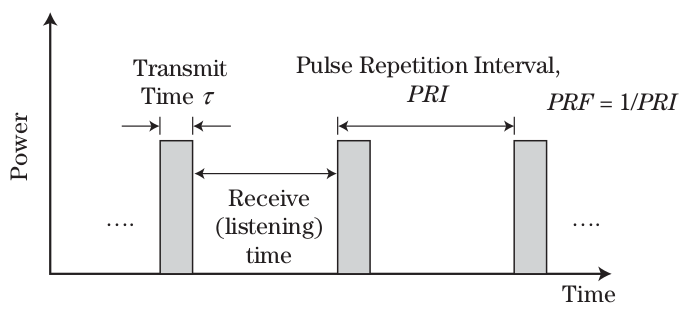
\includegraphics[width=10cm]{pulsedWaveform}
 \caption{Forma de onda de un radar pulsado \cite{Richards2010}.}
 \label{fig:pulsedWaveform}
\end{figure}


\subsection{Onda continua}

Generalmente este tipo de radares utilizan una configuración biestática, implicando que el transmisor se encuentre separado del receptor, para aumentar la aislación entre las antenas. Pero, como la aislación no es perfecta, utilizan baja potencia de transmisión. Por lo tanto, sólo son utilizados en aplicaciones de rangos cortos. Aunque hay sistemas complejos de radares de onda continua como iluminadores en sistemas de control de fuego, misiles semi activos, y rastreadores, también los hay con esquemas simples, aplicados en radares de velocidad, altímetros y sensores de proximidad \cite{Richards2010}. La figura \ref{fig:continuousWaveform} muestra un ejemplo de una modulación diente de sierra.

Dado que la transmisión es continua, la determinación del tiempo de ida y vuelta, del inglés round-trip time, de la señal electromagnética (EM) transmitida, por ende la distancia del blanco iluminado, debe realizarse cambiando las características de la señal. Por ejemplo modificando su frecuencia a través del tiempo. Esta técnica de modulación en frecuencia (FM) introduce una marca de tiempo en la onda EM, permitiendo así la determinación de la distancia al blanco.

\begin{figure}[H]
 \centering
 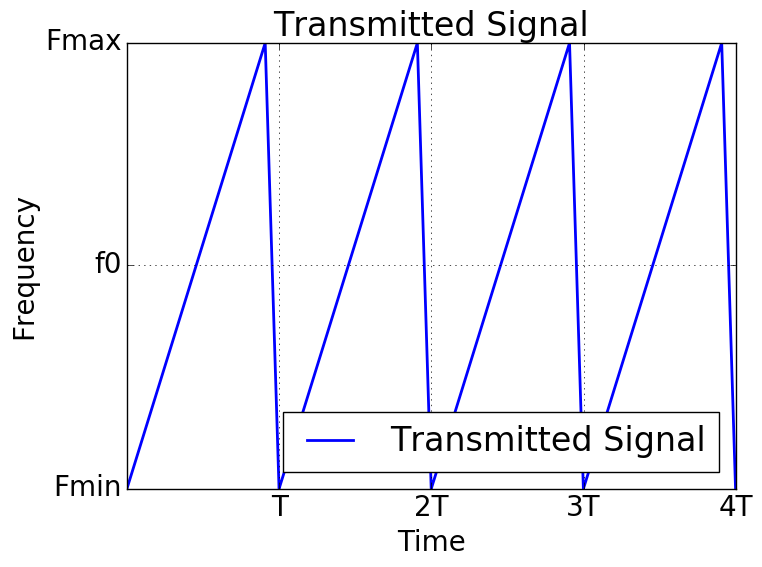
\includegraphics[width=8cm]{sawtoothSignal}
 \caption{Forma de onda de la señal transmitida por un radar FMCW.}
 \label{fig:continuousWaveform}
\end{figure}

En el presente trabajo de tesis, como se desea posicionar el cuerpo a una distancia del orden de los metros, se opta por utilizar este esquema de radares. Definiéndose de esta forma el requerimiento \ref{req:l1_radarType}.


\section{Ambigüedades en mediciones de rango} \label{sc:ambiguity}

Como la distancia a un cuerpo iluminado se mide determinando el tiempo de ida y vuelta entre la señal transmitida y el eco recibido, si dicho tiempo es mayor que el PRI, el sistema determina erróneamente dicha distancia. Este error es el llamado ambigüedad.

En la figura \ref{fig:ambiguity} se muestra un ejemplo de este efecto para un radar pulsado. Hay dos blancos, el primero a una distancia cercana y el segundo a una lejana, de tal forma, que el tiempo de ida y vuelta es mayor que el PRI. Se puede observar que el eco de la señal transmitida en el primer período del segundo blanco llega a la antena durante el tiempo de recepción del segundo período transmitido, logrando así un error en la estimación de la distancia a este blanco.

Para evitar tener ambigüedades, se debe incrementar el PRI lo suficiente para que todos los blancos estén dentro del máximo tiempo de ida y vuelta detectable.

\begin{figure}[H]
 \centering
 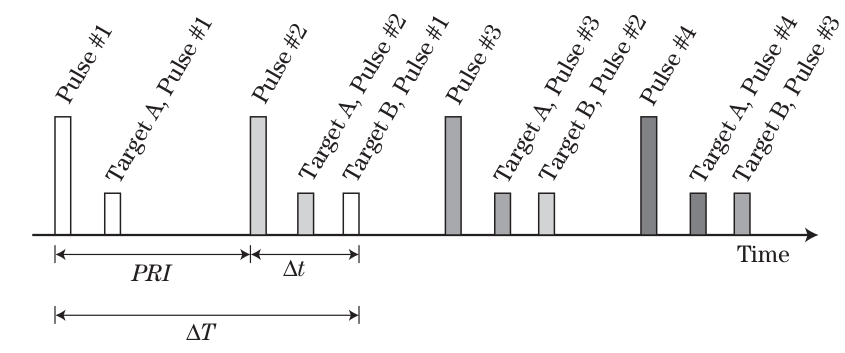
\includegraphics[width=10cm]{ambiguity}
 \caption{Ambigüedades en mediciones de rango en un radar pulsado \cite{Richards2010}.}
 \label{fig:ambiguity}
\end{figure}

En el caso de los radares FMCW, la determinación de la distancia está relacionada con la frecuencia de la señal a procesar y, dado que se transmite constantemente e independientemente de la posición en que estén los blancos iluminados, siempre habrá un solapamiento entre el pulso transmitido siguiente y la señal recibida del pulso anterior. En la figura \ref{fig:fmcwAmbiguity} se puede apreciar dicho solapamiento entre los tiempos T y T1. Como la señal a procesar es la multiplicación entre el pulso transmitido y recibido, la frecuencia recibida en el intervalo T y T1 varía a causa de la mezcla entre pulsos consecutivos, ver figura \ref{fig:modulationDelayed}.

Para evitar errores en el cálculo de la estimación en la frecuencia, se puede aplicar un retraso en la señal a procesar, evitando tomar las muestras correspondientes al solapamiento entre pulsos o se puede transmitir interrumpiendo durante un tiempo equivalente o superior al máximo tiempo de ida y vuelta de la señal admitido \cite{Varavin2007a}. Por último, para disminuir errores en dicho cálculo se aumenta la duración del tiempo T, aumentando el ancho de banda o disminuyendo la pendiente de la rampa de la señal modulada.

\begin{figure}[H]
  \centering
  \begin{subfigure}[t]{0.49\textwidth}
    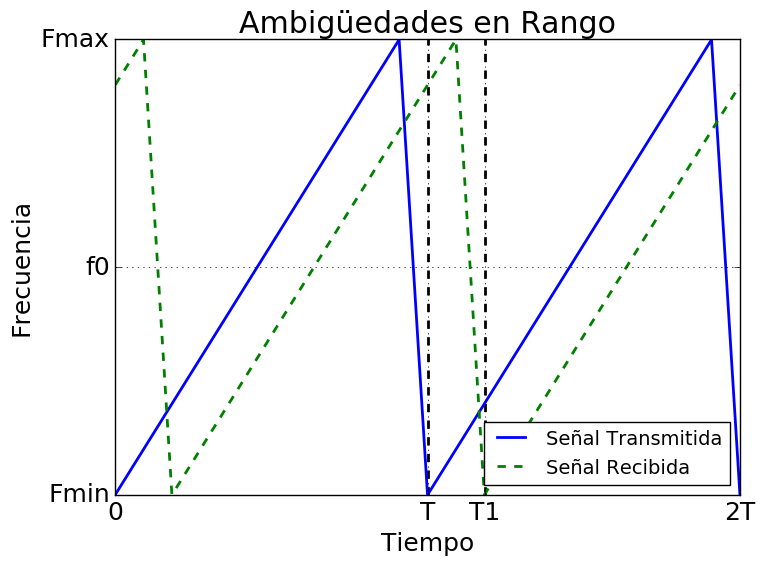
\includegraphics[width=7.5cm]{FMCWambiguity}
    \caption{Señal transmitida y recibida en función del tiempo}
    \label{fig:fmcwAmbiguity}   
  \end{subfigure}
  \begin{subfigure}[t]{0.49\textwidth}
    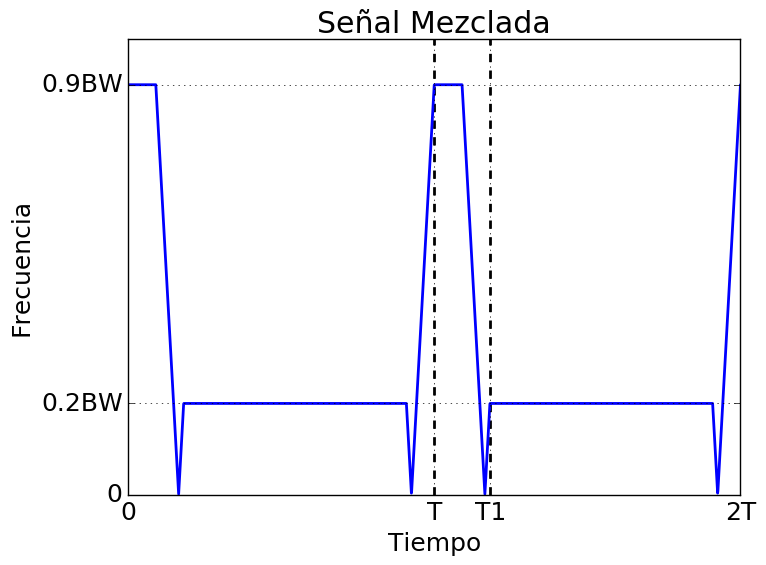
\includegraphics[width=7.5cm]{receivedFrequency}
    \caption{Frecuencia recibida de la señal a procesar.}
    \label{fig:modulationDelayed}
  \end{subfigure}             
  \caption{Ambigüedades en un radar FMCW.}
\end{figure}

\section{Antenas}

Una antena es definida como la estructura de transición entre el espacio libre y un dispositivo guía, como se muestra en la 
figura \ref{fig:antenna}. El dispositivo guía o línea de transmisión puede ser un cable coaxial o un tubo hueco (guía de 
onda), el cual es utilizado para transportar energía electromagnética desde la fuente de transmisión a la antena, o desde la 
antena al receptor. En el primer caso sería una configuración de antena transmisora y en el segundo, receptora \cite{Balanis2012}.
\begin{figure}[H]
 \centering
 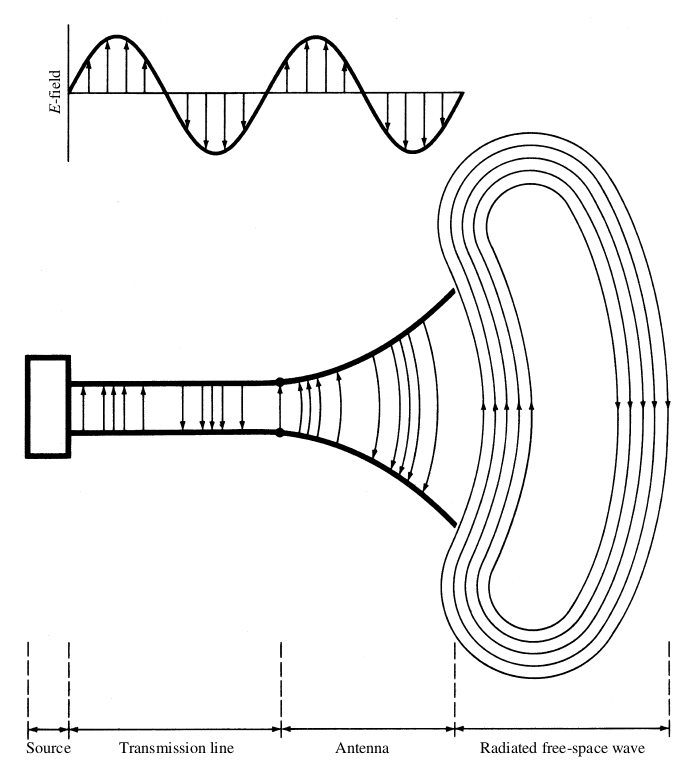
\includegraphics[width=10cm]{antenna}
 \caption{Antena como un dispositivo de transmisión \cite{Balanis2012}.}
 \label{fig:antenna}
\end{figure}

Hay una amplia variedad de antenas en la actualidad, en la tabla \ref{tab:type_antennas} se puede observar una agrupación 
simplificada.

\begin{table}[H]
  \caption{Características de cada grupo principal de antenas}
  \footnotesize
  \centering
  \begin{tabular}{l p{12.5cm}}
  \toprule
  \textbf{Tipo Antena} & \textbf{Características} \tabularnewline
  \midrule
  Cable & Son el tipo de antenas más utilizados porque se las puede en autos, edificios, barcos, sistemas aeroespaciales. Hay distintas formas de estas antenas, como monopolos, dipolos, lazos y hélices o alguna otra configuración. Los usos más comunes de los monopolos son para radios AM/FM y walkie talkies; de los dipolos son para antenas de canales de tv VHF o antena de televisión analógico; y de lazos son para receptoras de canales UHF de tv o receptores de AM \cite{Balanis2012}. \tabularnewline

  Apertura & Son el principal tipo de antenas direccionales utilizadas en frecuencias microondas. Consisten en una antena
  del tipo dipolo o Lazo junto a una estructura que guía las ondas en una dirección determinada. Este tipo de antenas son muy utilizadas en el ámbito aéreo y espacial dado que se pueden empotrar en la superficie del avión o satélite. A su vez, se los puede cubrir con un material dieléctrico para protegerlos de las condiciones ambientales \cite{Balanis2012}. \tabularnewline
  
  Microstrip & Consisten en un patch metálico sobre un sustrato. Dicho patch puede tomar distintas formas, aunque, la rectangular y circular son las más populares dada su facilidad de fabricación y por sus características de radiación, como por ejemplo la baja radiación en la polarización cruzada. Este tipo de antenas son simples, de bajo costo de fabricación, son mecánicamente robustas si se las monta en superficies rígidas y muy versátiles en términos de frecuencias de resonancia, polarización, diagramas de radiación e impedancias. Son muy utilizadas en aplicaciones aeroespaciales y celulares \cite{Balanis2012}. \tabularnewline

  Conjunto & Muchas aplicaciones requieren características de radiación que pueden no ser alcanzables con un único elemento sino que por un conjunto de elementos en una distribución eléctrica y geométrica determinada. La distribución adoptada afecta en distintos aspectos al diagrama de radiación. Algunos usos son Transmisión de canales de televisión en VHF, detección de misiles, comunicaciones satelitales \cite{Balanis2012}. \tabularnewline
  
  Reflectores & Estas antenas son utilizadas para comunicaciones a largas distancias, para transmitir y recibir señales que tienen que recorrer kilómetros. Un estilo muy común de este tipo de antenas es el reflector parabólico, el diámetro máximo construido es de $\SI{305}{\meter}$, necesario por la gran ganancia requerida para transmitir o recibir señales a miles de kilómetros. Otro tipo de reflector no tan común como la parábola es el corner reflector \cite{Balanis2012}. \tabularnewline

  Lentes & Son utilizadas principalmente para transformar energía divergente en ondas planas, de esta forma se previene  transmisión en direcciones indeseadas. Se pueden utilizar en casi las mismas aplicaciones que los reflectores parabólicos, especialmente en altas frecuencias. Para bajas frecuencias no son utilizadas dado que sus dimensiones y peso se tornan inmanejables \cite{Balanis2012}. \tabularnewline
  \bottomrule 
  \end{tabular}
  \label{tab:type_antennas}
\end{table}

Por la simplicidad de construcción, en la presente tesis se opta por utilizar el tipo de antena monopolo, de esta forma se desprende el requerimiento \ref{req:l2_antenna}. A continuación se detalla este tipo de antenas comparándolo con su contraparte, el dipolo.


\subsection{Monopolos y Dipolos}

Un monopolo es un dipolo que ha sido dividido a la mitad de su punto de alimentación central y es alimentado contra un plano de tierra, el cual actúa como un estilo de espejo eléctrico \cite{arrl2007}. La figura \ref{fig:monopoles} compara un dipolo de $\frac{\lambda}{2}$ con un monopolo de $\frac{\lambda}{4}$ de longitud. La antena imagen, para el monopolo, está representada con una línea punteada debajo del plano de tierra. La misma forma la segunda mitad de la antena, transformando funcionalmente al monopolo en un dipolo.

\begin{figure}
 \centering
 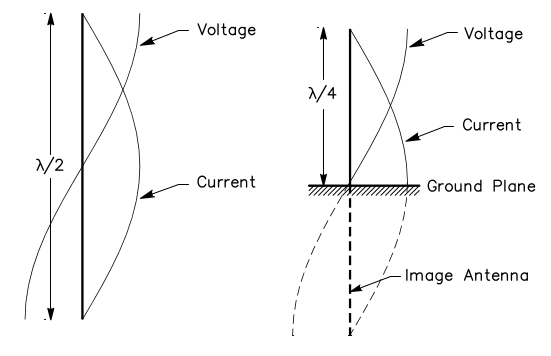
\includegraphics[width=10cm]{monopoleVsDipole}
 \caption{Un dipolo de longitud $\frac{\lambda}{2}$ y su contraparte de $\frac{\lambda}{4}$ con plano de tierra \cite{arrl2007}.}
 \label{fig:monopoles}
\end{figure}

Las cargas y corrientes en un monopolo son las mismas que la mitad superior del dipolo, aunque la tensión en sus terminales es solo la mitad, y el mismo campo eléctrico en la mitad de distancia también implica la mitad de tensión. Por lo tanto, la impedancia de entrada de un monopolo se ve disminuida a la mitad que la de su contraparte \cite{Stutzman2013},
\begin{equation}
\bm{Z}_{mono} = \dfrac{\bm{V}_{mono}}{\bm{I}_{mono}} = \dfrac{\frac{1}{2}\bm{V}_{dipolo}}{\bm{I}_{dipolo}} = \dfrac{1}{2}\bm{Z}_{dipolo}
\end{equation}
Es importante notar que la nomenclatura para valores complejos es la de utilizar letras en negrita y en itálica.

El diagrama de radiación de un monopolo sobre un plano de tierra perfecto es el mismo que el de un dipolo con las mismas dimensiones en espacio libre dado que los campos por encima del plano imagen son los mismos, ver figura \ref{fig:radingPatternDipole}. Por lo tanto, la potencia radiada por un monopolo sobre un plano de tierra perfecto es la mitad que la del dipolo en espacio libre porque la distribución de potencia es igual, pero solo sobre la mitad del espacio. Dando como resultado, el ancho del haz radiado sea la mitad que el del dipolo, llevando a que la directividad sea el doble \cite{Stutzman2013},
\begin{equation}
  D_{mono} = \dfrac{4\pi}{\Omega_{mono}} = \dfrac{4\pi}{\frac{1}{2}\Omega_{dipolo}} = 2D_{dipolo}
\end{equation}

En la práctica, un plano de tierra no puede ser infinito, aunque un plano de tierra con un radio aproximadamente igual de largo que la longitud del elemento activo resulta una solución viable. Aunque sin un sistema de tierra bien elaborado, la eficiencia del monopolo resulta drásticamente deteriorada llegando a ser menor al $\SI{50}{\percent}$ con respecto a su contraparte. Si la longitud es menor que $\frac{\lambda}{4}$ puede ser mucho peor \cite{arrl2007}.

\begin{figure}
  \centering
  \begin{subfigure}[b]{0.4\textwidth}
    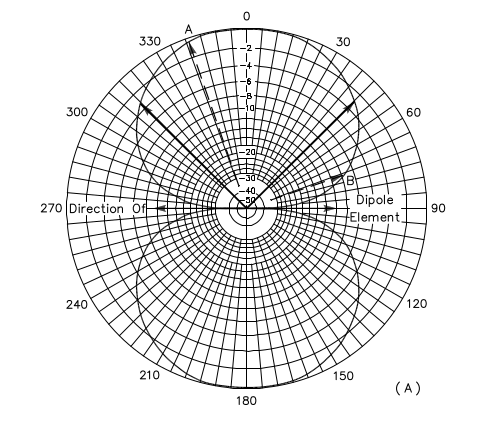
\includegraphics[width=6cm]{radiatingPatternDipole1}
    % \caption{Esquemático del modulador.}
  \end{subfigure}
  \begin{subfigure}[b]{0.4\textwidth}
    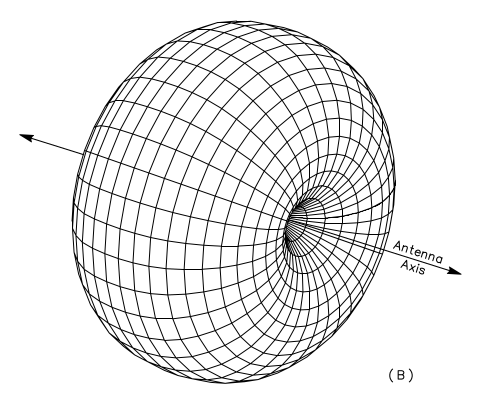
\includegraphics[width=6cm]{radiatingPatternDipole2}
    % \caption{PCB del modulador.}
  \end{subfigure}             
  \caption{Diagrama de radiación de un dipolo \cite{arrl2007}.}
  \label{fig:radingPatternDipole}
\end{figure}

La directividad de un monopolo de cuarto de longitud de onda es el doble que el un dipolo de media longitud de onda en espacio libre \cite{Stutzman2013},
\begin{equation}
  D = 2(1.64) = 3.28 = \SI{5.16}{\dB}
\end{equation}

La impedancia de entrada de un monopolo de un cuarto de longitud de onda infinitesimalmente fino resulta \cite{Stutzman2013},
\begin{equation}
  \bm{Z} = ~ (72 + j42.5) = 36 + j\SI{21.3}{\Omega}
\end{equation}

\subsection{Polarización} \label{sc:polarization}

La polarización de una onda radiada se la define como la propiedad de una onda electromagnética describiendo la variación en tiempo de la dirección y la magnitud relativa del vector del campo eléctrico; específicamente, la figura trazada en función del tiempo por la extremidad del vector en un lugar fijo en el espacio, y el sentido en que es trazado, como observado a lo largo de la dirección de propagación. Por lo tanto, la polarización es la curva trazada por la punta del vector que representa el campo eléctrico instantáneo \cite{Balanis2012}.

La polarización se puede clasificar como lineal, circular o elíptica (ver figura \ref{fig:hvPolarizations}). Si el vector que describe el campo eléctrico en un punto del espacio en función del tiempo recorre un trayecto a lo largo de una línea, se dice que el campo es linealmente polarizado (horizontalmente y/o verticalmente). En general, la figura trazada por el campo eléctrico es una elipse, nombrada polarización elíptica. La polarización lineal y circular son casos especiales de la elíptica \cite{Vita2012}.

\begin{figure}[H]
  \centering
  \begin{subfigure}[b]{0.49\textwidth}
    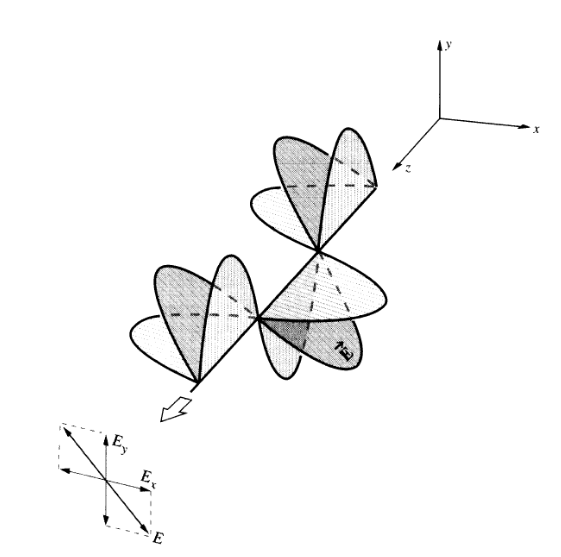
\includegraphics[width=7cm]{linearPolarization}
    \caption{Polarización lineal.}
  \end{subfigure}
  \begin{subfigure}[b]{0.49\textwidth}
    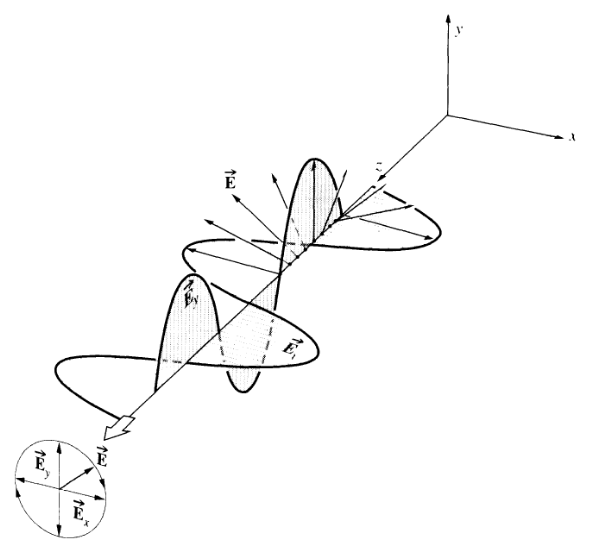
\includegraphics[width=7cm]{circularPolarization}
    \caption{Polarización circular.}
  \end{subfigure}
  \caption{Distintos tipos de polarizaciones \cite{Hecht2002}.}
  \label{fig:hvPolarizations}
\end{figure}

Para el caso de esta tesis, las antenas a construir son polarimétricas. Esto implica que poseen dos componentes, una Horizontal (H) y otra Vertical (V). Con esto se define el requerimiento \ref{req:l2_polarization}.


\section{Parámetros S} 

La sigla S deriva de la palabra dispersión. Para altas frecuencias, es conveniente describir una determinada red en términos de ondas en vez de tensiones o corrientes. Esto permite una definición más sencilla de planos de referencia. Por razones prácticas, la descripción en términos de ondas entrantes y salientes ha sido introducida. Ahora, una red de 4 polos se transforma en 2 puertos y $2n$ polos se transforman en $n$ puertos. En el caso de un número impar de polos (ej. 3 polos), un punto de referencia puede ser elegido, atribuyendo un polo igualmente a dos puertos. Por lo tanto 3 polos se convierten en 3 + 1 polo correspondiendo a 2 puertos. Como una regla general, para cantidades impares de polos, siempre se agrega un polo extra \cite{Caspers}.

\begin{figure}[H]
 \centering
 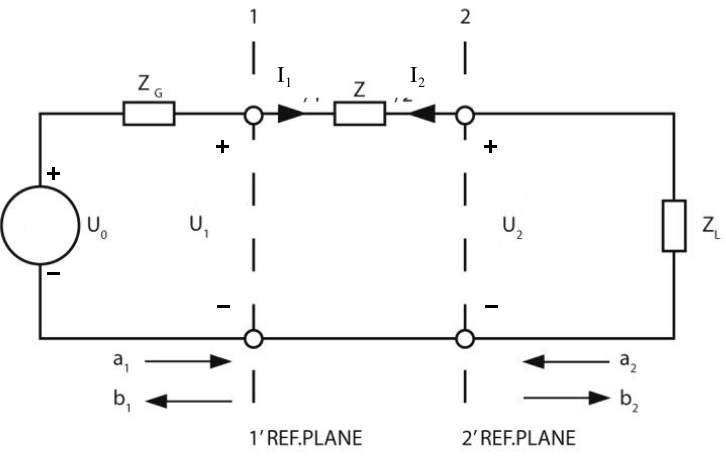
\includegraphics[width=10cm]{sParameters1}
 \caption{Ejemplo de una red de 2 puertos: circuito serie \cite{Caspers}}
 \label{fig:esquema_serie}
\end{figure}

Tomando como ejemplo una red de 2 puertos compuesta por una sola impedancia $\bm{Z}$ conectada en serie (figura \ref{fig:esquema_serie}). Las impedancias de la fuente y de la carga son $\bm{Z_G}$ y $\bm{Z_L}$ respectivamente. Si $\bm{Z}=0$ y $\bm{Z_L} = \bm{Z_G}$ (para el caso de $\bm{Z_G}$ real) la carga está adaptada. En este caso se obtiene una máxima transferencia de potencia y $\bm{U_1} = \bm{U_2} = \bm{U_0}/2$. Notar que todas las tensiones y corrientes son valores pico. Se supone que las líneas que unen los componentes poseen longitud eléctrica igual a 0. Las conexiones con una longitud eléctrica finita están dibujadas como una doble línea. A continuación se relacionará $\bm{U_0}$, $\bm{U_1}$ y $\bm{U_2}$ a $\bm{a}$ y $\bm{b}$.


\subsection{Definición de "ondas de potencia"}

Las ondas incidentes al puerto son $\textbf{a}=(\bm{a_1}, \bm{a_2}, \bm{a_3}, ..., \bm{a_n})$, las ondas salientes, o reflejadas, del puerto son $\textbf{b}=(\bm{b_1}, \bm{b_2}, \bm{b_3}, ..., \bm{b_n})$. Por definición, las corrientes incidentes son positivas y las salientes negativas. La onda $\bm{a_1}$, incidente al puerto 1, es derivada de la tensión entrante a la carga balanceada.

Para hacer que ésta definición sea consistente con la ley de la conservación de la energía. La tensión es normalizada a $\sqrt{\bm{Z_0}}$. $\bm{Z_0}$ es, en general una impedancia de referencia arbitraria, que usualmente se la utiliza como la impedancia característica de la línea (ej, $\bm{Z_0} = 50 \Omega$). Y, cuando todas las impedancias son iguales ($\bm{Z_G} = \bm{Z_L} = \bm{Z_0}$), se dice que la línea está adaptada y no hay onda reflejada. Las definiciones de $\bm{a_1}$ y $\bm{b_1}$ son
\begin{equation}
\begin{aligned}
  \bm{a_1} &= \dfrac{\bm{U_0}}{2\sqrt{\bm{Z_0}}}= \dfrac{\textrm{onda de tensión incidente (puerto 1)}}{\sqrt{\bm{Z_0}}}=\dfrac{\bm{U_1}^{inc}}{\sqrt{\bm{Z_0}}} \\
  \bm{b_1} &= \dfrac{\bm{U_1}^{refl}}{2\sqrt{\bm{Z_0}}}= \dfrac{\textrm{onda de tensión reflejada (puerto 1)}}{\sqrt{\bm{Z_0}}}
\end{aligned}
\end{equation}

Notar que \textbf{a} y \textbf{b} tienen las unidades de $\sqrt{\textrm{potencia}}$.

La potencia incidente al puerto 1, $P_{inc}$, es simplemente la potencia entregada por la fuente, mientras que la potencia saliente del puerto 1, $P_{refl}$, viene de la onda de tensión reflejada.
\begin{equation}
\begin{aligned}
  P_1^{inc} &= \dfrac{1}{2}|\bm{a_1}|^2= \dfrac{|\bm{U_1}^{inc}|^2}{2\bm{Z_0}}=\dfrac{|\bm{I_1}^{inc}|^2}{2}\bm{Z_0} \\
  P_1^{refl} &= \dfrac{1}{2}|\bm{b_1}|^2= \dfrac{|\bm{U_1}^{refl}|^2}{2\bm{Z_0}}=\dfrac{|\bm{I_1}^{refl}|^2}{2}\bm{Z_0} \\
\end{aligned}
\end{equation}

En el caso de una desadaptación de la impedancia de carga $\bm{Z_L}$, parte de la potencia será reflejada a través del puerto 2 (potencia incidente al puerto 2).
\begin{equation}
P_2^{inc}=\dfrac{1}{2}|\bm{a_2}|^2
\end{equation}

Se ha definido $\bm{a_1} = \bm{U_0}/2\sqrt{\bm{Z_0}} = \bm{U}^{inc}/\sqrt{\bm{Z_0}}$ con la onda de tensión incidente $\bm{U}^{inc}$. Como analogía se la puede definir como $\bm{a_1} = \bm{I}^{inc}\sqrt{\bm{Z_0}}$ con la onda incidente de corriente $\bm{I}^{inc}$. Utilizando ambas, se obtiene la definición general de las ondas incidentes $\bm{a_i}$ y reflejadas $\bm{b_i}$ de un puerto.
\begin{equation}
\begin{aligned}
  \bm{a_i} &= \dfrac{\bm{U_i} + \bm{I_i}\bm{Z_0}}{2\sqrt{\bm{Z_0}}} \\
  \bm{b_i} &= \dfrac{\bm{U_i} - \bm{I_i}\bm{Z_0}}{2\sqrt{\bm{Z_0}}}
\end{aligned}
\label{eq:waves}
\end{equation}

Solucionando este sistema de ecuaciones, $\bm{U_i}$ y $\bm{I_i}$ pueden ser obtenidas de $\bm{a_i}$ y $\bm{b_i}$ como
\begin{equation}
\begin{aligned}
  \bm{U_i} &= \sqrt{\bm{Z_0}}(\bm{a_i} + \bm{b_i}) = \bm{U_i}^{inc} + \bm{U_i}^{refl}\\
  \bm{I_i} &= \dfrac{1}{\sqrt{\bm{Z_0}}}(\bm{a_i} - \bm{b_i}) = \dfrac{\bm{U_i}^{refl}}{\bm{Z_0}}
\end{aligned}
\end{equation}


\subsection{La matriz de parámetros S}

La relación entre $\bm{a_i}$ y $\bm{b_i}$ (siendo $i=1..n$) puede ser escrito como un sistema de n ecuaciones lineales (siendo la variable independiente $\bm{a_i}$ y $\bm{b_i}$ la dependiente)
\begin{equation}
\begin{aligned}
  \bm{b_1} = \bm{S}_{11}\bm{a_1} + \bm{S}_{12}\bm{a_2} \\
  \bm{b_2} = \bm{S}_{21}\bm{a_1} + \bm{S}_{22}\bm{a_2}
\end{aligned}
\label{eq:s_matrix}
\end{equation}

Escrito de forma matricial: \textbf{b} = \textbf{Sa}

El significado físico de los parámetros S es:
\begin{itemize}
  \item $\bm{S}_{11}$: es el coeficiente de reflexión con la salida de la red terminada en una carga adaptada ($\bm{a_2} = 0$).
  \item $\bm{S}_{21}$: es la transmisión en directa (del puerto 1 al 2)
  \item $\bm{S}_{12}$: es la transmisión en inversa (del puerto 2 al 1)
  \item $\bm{S}_{22}$: es el coeficiente de reflexión de la salida.
\end{itemize}

Al medir todos los parámetros S de una red de n puertos, todos los puertos deben estar terminados con una carga adaptada. Utilizando las ecuaciones \ref{eq:waves} y \ref{eq:s_matrix} se obtiene el coeficiente de reflexión de una impedancia $\bm{Z_L}$ conectada a un generador de impedancia de salida $\bm{Z_0}$ (Figura \ref{fig:esquema_serie}, caso $\bm{Z_G} = \bm{Z_0}$ y $\bm{Z} = 0$)
\begin{equation}
\bm{S}_{11} = \dfrac{\bm{b_1}}{\bm{a_1}}\bigg|_{\bm{a_2}=0} = \dfrac{\bm{U_1} - \bm{I_1}\bm{Z_0}}{\bm{U_1} + \bm{I_1}\bm{Z_0}} = \dfrac{\bm{Z_L} - \bm{Z_0}}{\bm{Z_L} + \bm{Z_0}} = \bm{\Gamma}
\end{equation}


\section{Procesamiento de la señal de un radar FMCW}

Hay distintos tipos de modulaciones con las que se puede transmitir utilizando dicho tipo de radar, las cuales están resumidas a continuación.

\begin{description}

\item[Modulación diente de sierra] En esta modulación se transmite una rampa en frecuencia con respecto al tiempo y es utilizada para distancias grandes combinado con una influencia despreciable de frecuencia doppler. Si se observara un blanco estático, el eco recibido solamente posee un desplazamiento en tiempo, en cambio, si está en movimiento se genera una frecuencia doppler. Dicho efecto desplaza la frecuencia de la señal recibida incrementándola, si el blanco se mueve hacia el radar, o decrementándola, si se aleja del mismo. En esta modulación el receptor no tiene forma de separar ambas frecuencias, por lo tanto, el efecto doppler es tomado como un error en la medición. Un ejemplo es un radar de navegación marítimo \cite{Basics2015}. En \cite{Varavin2007a, Shen} se detalla el procesamiento de este tipo de modulación para un radar FMCW.

\item[Modulación Triangular] En un cambio de frecuencia de forma triangular, se pueden utilizar ambas pendientes para medir la distancia al cuerpo. Sin efecto doppler, el desplazamiento en tiempo del eco, por ende la diferencia en frecuencia es la misma tanto para la pendiente positiva como negativa. En cambio, como el efecto doppler incrementa o decrementa las frecuencias del eco, en una de las pendientes la diferencia de frecuencias se aumenta, pero para la otra decrece en la misma medida. Haciendo un análisis y comparando los resultados de cada pendiente de forma separada, se permite determinar fácilmente la diferencia en frecuencia $\Delta f$ con respecto a la frecuencia doppler $f_D$ \cite{Basics2015}. En \cite{Chang2006, Kurt2007} se detalla el procesamiento de este tipo de modulación para un radar FMCW.

\item[Modulación cuadrada o FSK] Esta modulación es utilizada para mediciones muy precisas de rango a distancias cortas. Se compara la fase de la señal recibida de las distintas frecuencias transmitidas. La mayor desventaja es que no se puede distinguir los ecos de distintos blancos iluminados y que el rango sin ambigüedades es muy chico \cite{Basics2015}.

\item[Modulación escalonada] Para detectar objetos con un mucho ruido del entorno, o clutter, para la distinción del objeto requiere alta resolución en rango. Esto se obtiene utilizando pulsos cortos y de gran ancho de banda, por lo tanto, se debe utilizar un receptor de gran ancho de banda, el cual es muy costoso. Para no utilizar un receptor de gran ancho de banda, se modula la frecuencia de forma escalonada en sucesivos pulsos, de esta forma, la resolución en rango no se ve comprometida \cite{steppedFreq}. A su vez, esta modulación se la utiliza para mediciones de interferometría y aumenta el rango de mediciones sin ambigüedades \cite{Basics2015}.

Es importante destacar que las señales que poseen una modulación del tipo rampa son llamadas chirps.

\end{description}

En esta tesis se utiliza la modulación diente de sierra dado que el radar es utilizado para realizar mediciones con blancos estáticos. De esta forma se define el requerimiento \ref{req:l2_mod}. La figura \ref{fig:sawtoothSignal} ilustra para un caso general los parámetros que definen dicha señal, los cuales son el ancho de banda de la señal transmitida ($BW$) y el período ($T$) o tiempo de repetición de dicho pulso ($PRT$).

\begin{figure}
 \centering
 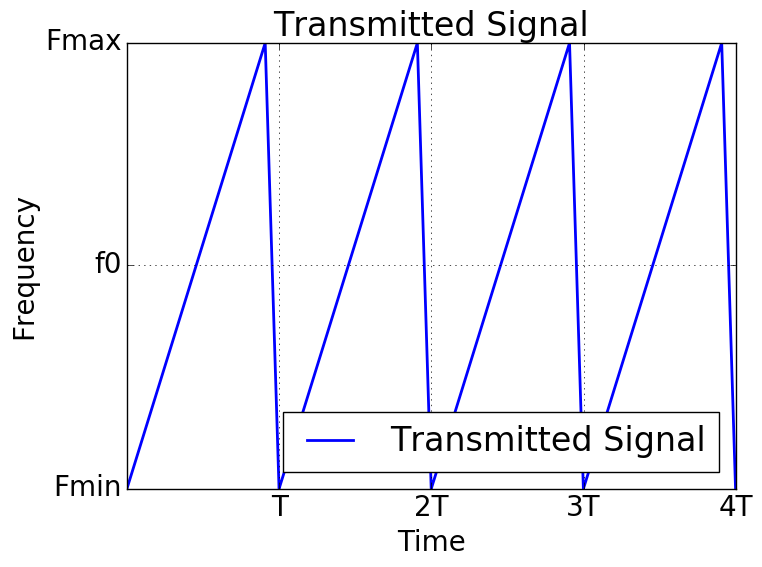
\includegraphics[width=10cm]{sawtoothSignal}
 \caption{Modulación diente de sierra de la señal a transmitir.}
 \label{fig:sawtoothSignal}
\end{figure}

Para extraer el efecto que el medio induce sobre la señal, es importante saber determinar la distancia a la cual está el cuerpo iluminado con respecto al radar. De esta forma se define el requerimiento \ref{req:l1_distance}. Para el desarrollo a continuación se asume que se está trabajando en campo lejano, con esta suposición el campo eléctrico y magnético de la onda transmitida y recibida son ortogonales a la dirección de la misma. En general, cuando se está a unas pocas longitudes de onda de distancia ya se cumple esta condición. En un monopolo se cumple a una distancia $r$ aproximadamente igual a $\lambda/ 6$ \cite{Richards2009}.


\subsection{Determinación de distancia}

Para determinar la distancia de un cuerpo iluminado se mide el tiempo de ida y vuelta de la señal transmitida. En la figura \ref{fig:roundTripTime} se muestra la modulación de una chirp transmitida por el radar y el eco recibido, producido por dicho blanco a una distancia $R$. Se puede observar que el tiempo de ida y vuelta de la señal está marcado como $\tau$.

\begin{figure}
 \centering
 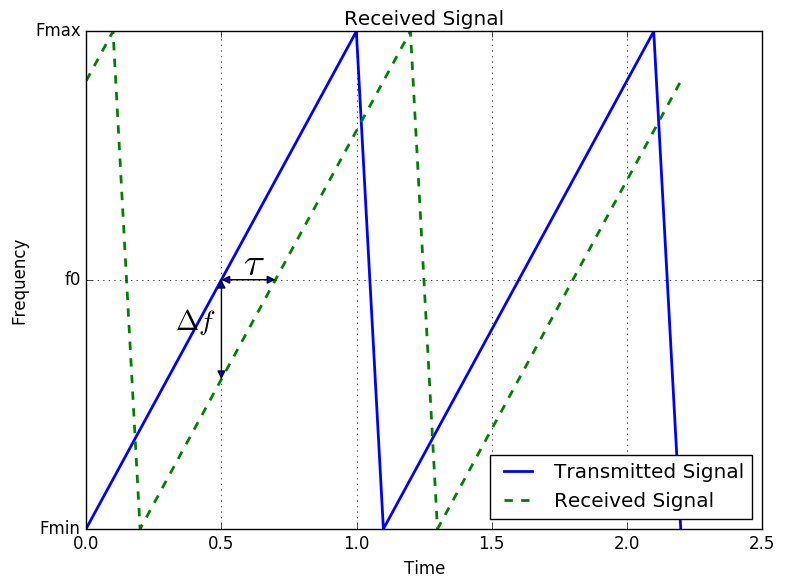
\includegraphics[width=10cm]{round-tripTime}
 \caption{Modulación diente de sierra de la señal a transmitir.}
 \label{fig:roundTripTime}
\end{figure}

La relación entre el tiempo de ida y vuelta $\tau$ y la distancia es,
\begin{equation}\label{eq:relDist}
  \tau = \dfrac{2R\sqrt{\varepsilon_r}}{c}
\end{equation}
donde $\varepsilon_r$ es la permitividad relativa del medio.

Este tipo de radares utiliza la relación entre la diferencia de tiempo $\tau$ y la diferencia en frecuencia, $\Delta f$, entre las señales transmitidas y recibidas,
\begin{equation}\label{eq:relFreqDist}
  \tau = \dfrac{T\Delta f}{B}
\end{equation}
donde $B$ es el ancho de banda de la señal y $T$ es el tiempo en que es barrido el BW, desde la frecuencia mínima a la máxima, sin contar el tiempo que tarda el generador en volver de la frecuencia máxima a la mínima. Por lo tanto utilizando las ecuaciones \ref{eq:relDist} y \ref{eq:relFreqDist} se puede determinar la distancia $R$ a partir de la señal recibida,
\begin{equation}\label{eq:receivedDist}
  R = \dfrac{T\Delta fc}{2B\varepsilon_r}
\end{equation}

Para determinar la resolución en distancia, se debe tener en cuenta que la misma está relacionada con la resolución espectral de la señal recibida. Asumiendo $T >> T_d$, el ancho de banda a $\SI{-3}{\dB}$ con respecto a su pico es igual a $1/T$ \cite{Brooker2005}. Es importante destacar que dicho valor es igual a la distancia entre las frecuencias nulas, dado que el espectro se corresponde a una sinc.
\begin{equation}\label{eq:resolutionDistance}
  \Delta R = \dfrac{c}{2B\sqrt{\varepsilon_r}}
\end{equation}

Se puede apreciar que la resolución en distancia obtenida, ecuación \ref{eq:resolutionDistance}, no depende ni del período ($T$) de la señal transmitida ni de su frecuencia central ($f_0$), solamente de su ancho de banda ($B$). Hay que tener en cuenta que las alinelidades de la señal modulada degradan la resolución obtenida, y la misma depende del ancho de banda, por lo tanto, la mayor resolución se obtiene tomando en cuenta ambos efectos \cite{Brooker2005}.

Como la distancia al cuerpo se determina midiendo la frecuencia de la señal recibida, o en su defecto el pico de la sinc en frecuencia, se pueden agregar ceros al final de la señal para aumentar la resolución de la FFT. Dicho proceso es llamado zero padding \cite{Oppenheim1990}.
\begin{equation}\label{eq:resolutionDistance2}
  \Delta R = \dfrac{c}{2B\sqrt{\varepsilon_r}p}
\end{equation}

Siendo $p$ la relación entre la frecuencia de muestreo $f$ de la señal y la cantidad de muestras $n$ utilizada para realizar la FFT.
\begin{equation}
  p = \frac{f}{n}
\end{equation}


\subsection{Determinación de la relación de fase}

Para determinar la fase del cuerpo iluminado es necesario realizar un análisis de la fase de la señal recibida. La figura \ref{fig:phaseSystem} muestra el recorrido de la señal, en particular centrando en el análisis que se está realizando.
\begin{figure}[htb]
 \centering
 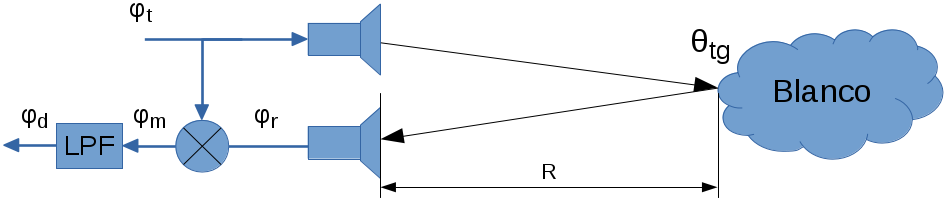
\includegraphics[width=10cm]{phaseMeasurement}
 \caption{Análisis de fase del sistema completo.}
 \label{fig:phaseSystem}
\end{figure}

La ecuación que define la modulación de cada período del pulso se encuentra descripta a continuación,
\begin{equation}
  f(t) = f_0 + \dfrac{B}{T}(t-\dfrac{T}{2}),\quad 0 \le t < T
  \label{eq:signalFrequency}
\end{equation}

donde $c$ es la velocidad de la luz, $\varepsilon_r$ es la constante dieléctrica del medio \cite{Brennan2014a} y $T$ es el tiempo en que es barrido el BW, desde la frecuencia mínima a la máxima, sin contar el tiempo que tarda el generador en volver de la frecuencia máxima a la mínima. Dado que la fase de una señal es la integral de su frecuencia sumada a una constante, se obtiene la fase instantánea transmitida a partir de la ecuación \ref{eq:signalFrequency},
\begin{equation}
  \varphi_t(t) = 2\pi f_0t + \dfrac{2\pi B}{2T}(t^2-Tt) + \phi_0,\quad 0 \le t < T
  \label{eq:signalFrequency2}
\end{equation}

El eco recibido por un objeto puntual en una distancia $R$ y desfasando la señal en $\theta$ llega al radar con la fase,
\begin{equation}
  \varphi_r(t) = w_0(t-\tau) + \dfrac{2\pi B}{2T}((t - \tau)^2-T(t - \tau)) + \theta + \phi_0,\quad 0 \le t < T
  \label{eq:signalFrequency3}
\end{equation}

donde $\tau$ es el tiempo ida y vuelta de la señal entre el transmisor y receptor del radar obtenido de la ecuación \ref{eq:relDist}.

Luego, en el mezclador, la señal recibida se la multiplica con la transmitida, por identidad trigonométrica, se obtiene
\begin{equation}
  x_m(t) = \dfrac{A_tA_r}{2}(\cos(\varphi_t(t)+\varphi_r(t)) + \cos(\varphi_t(t)- \varphi_r(r)))
  \label{eq:signalFrequency4}
\end{equation}

Donde $A_r$ es la amplitud de la señal recibida, la cual es modificada por el ida y vuelta del medio y por el blanco donde se genera el eco de la señal.

Que, luego del filtro pasa bajos, el primer término de la ecuación \ref{eq:signalFrequency4}, el cual posee una frecuencia de $2w_0$, resulta completamente atenuado, quedando solamente el término con la resta de fases,
\begin{equation}
  x_d(t) = \dfrac{A_tA_r}{2}\cos(w_0\tau + \dfrac{2\pi B\tau}{T}(t - \dfrac{T}{2}) - \dfrac{2\pi B\tau^2}{2T} - \theta)
  \label{eq:signalFrequency5}
\end{equation}

Es importante notar que la fase inicial de transmisión se elimina, por lo tanto no importa cual es la fase inicial de cada pulso
transmitido ni su variación entre pulsos. Para determinar la frecuencia de la señal recibida se deriva la ecuación \ref{eq:signalFrequency5}, 
\begin{equation}\label{eq:beatFreq}
  w_d = \dfrac{2\pi B\tau}{T} \rightarrow f_d = \dfrac{B\tau}{T}
\end{equation}

Se puede observar que el resultado obtenido es coherente con el resultado de la ecuación \ref{eq:relFreqDist}, el cual muestra la relación entre el round-trip time y la diferencia en frecuencia entre la señal transmitida y recibida.

Del resultado de la ecuación \ref{eq:signalFrequency5} se observa que la fase de la señal recibida está compuesta por cuatro términos.
\begin{itemize}
  \item $w_0\tau$ es el término utilizado para determinar distancias con alta precisión en blancos conocidos \cite{Brennan2014a}.
  \item $\dfrac{2\pi B\tau}{T}(t - \dfrac{T}{2})$ es un término de fase lineal con el tiempo que representa la frecuencia de la señal.
  \item $\dfrac{2\pi B\tau^2}{2T}$ es un offset en la señal, usualmente pequeño.
  \item $\theta$ es el término de fase originada por el blanco donde incidió la señal transmitida por el radar.
\end{itemize}

Para obtener el término de la fase originada por el blanco, $\theta$, primero se calcula la FFT de la señal recibida y se mide la fase del pico de la sinc, $\varphi_d$. Si no se realiza ninguna rotación a la señal en el momento del cálculo, el valor de $t$ correspondiente al segundo término es igual a 0. Luego, se debe restar dicho valor a la fase de los primeros tres términos correspondientes a la la distancia medida, 
\begin{equation}\label{eq:phaseMeasurement}
  \theta =  w_0\tau - \pi B\tau - \dfrac{\pi B\tau^2}{T} - \varphi_d  = \dfrac{2w_0R}{c} - \dfrac{2\pi BR}{c} - \dfrac{4\pi BR^2}{Tc^2} - \varphi_d
\end{equation}

Para utilizar la ecuación anterior, es fundamental que la diferencia de fase entre dos pulsos consecutivos en frecuencia sea menor que $2\pi$. Para ello, se realiza zero padding en la señal previo al cálculo de la FFT.

% Si se quisiera utilizar $w_0\tau$ para calcular la distancia, primero se tiene que hacer zero padding en la señal (para calcular la frecuencia de round trip time) de manera tal que la diferencia de fase entre dos pulsos consecutivos en frecuencia (que estan totalmente relacionados a $\Delta R$) sea menor que $2\pi$. Con esto, el $\Delta R$ al que está relacionado el pico de frecuencia entre dichos pulsos se puede determinar univocamente. La relación entre la fase y dicha distancia es $\Delta R = \frac{\lambda\phi}{4\pi}$, está dividido por 4 porque la distancia medida es el doble a la distancia entre el radar y el obteto iluminado.

% Sabiendo que la relación entre la distancia y la frecuencia medida, expresada en \ref{eq:beatFreq}, la máxima diferencia de distancia en que puede estar el objeto iluminado es igual a $\Delta R = \frac{c}{2B\sqrt{\varepsilon_r}}$, $\Delta f_d = \frac{1}{T}$ dado que es la resolución el frecuencia. Por lo tanto, la diferencia de fase es.

% \begin{equation}
%   \Delta(\omega_0\tau) = \dfrac{\omega_02\Delta R \sqrt{\varepsilon_r}}{c} = \dfrac{\omega_c}{B} = \dfrac{2\pi f_0}{B}
% \end{equation}


% \mynote{however, the phase indicated by an FFT is that at the start of the sample, at t = 0. It is therefore necessary to rotate the deramped (time-domain) waveform so that the centre of the waveform aligns with the start of the sample, t = 0, prior to FFT processing \cite{Brennan2014a}}

% \mynote{For processing convenience, it would be highly desirable if
% the phase relating to a point target located at the centre of each range bin is normalised to zero. This can be achieved by weighting the FFT-processed deramped waveform by a reference array equal to the phase conjugate of the expected phase at the centre of each range bin}

% \mynote{Seleccionar una función de ventana no es una tarea simple. Cada función de ventana tiene sus propias características y aptitud para diferentes aplicaciones. Para elegir una función de ventana, usted debe calcular el contenido de la frecuencia de la señal.
% Si la señal contiene componentes de frecuencia de fuerte interferencia alejados de la frecuencia de interés, elija una ventana con un rango alto de caída del lóbulo lateral.
% Si la señal contiene fuertes señales de interferencia cerca de la frecuencia de interés, elija una función de ventana con un nivel bajo de lóbulo lateral máximo.
% Si la frecuencia de interés contiene dos o más señales muy cerca una de la otra, la resolución espectral es importante. En este caso, es mejor elegir una ventana con un lóbulo principal muy estrecho.
% Si la precisión de la amplitud de un solo componente de frecuencia es más importante que la ubicación exacta del componente en un contenedor de frecuencia determinado, elija una ventana con un lóbulo principal amplio.
% Si el espectro de la señal es más bien plano o de banda ancha en el contenido de frecuencia, utilice la ventana uniforme o ninguna ventana.
% En general, la ventana Hanning (Hann) es satisfactoria en el 95\% de los casos. Tiene buena resolución de frecuencia y menor fuga espectral. Si no conoce la naturaleza de la señal, pero desea aplicar una ventana, comience con la ventana de Hann.
% http://www.ni.com/white-paper/4844/es/}


% \mynote{el mismo libro \cite{Richards2009} tiene una buena definicion con un buen grafico de polarización.}

\subsection{Determinación de la relación de amplitud}


Para determinar la ganancia del blanco, se debe realizar un análisis de potencia en todo el sistema, el cual se ilustra en la figura  \ref{fig:powerAnalysis}. Se puede observar que la señal transmitida posee atenuaciones por el medio en que la señal es transmitida y recibida, el blanco, las ganancias de transmisión y recepción de las antenas, el mezclador del receptor y el filtro pasa bajos. 

\begin{figure}
 \centering
 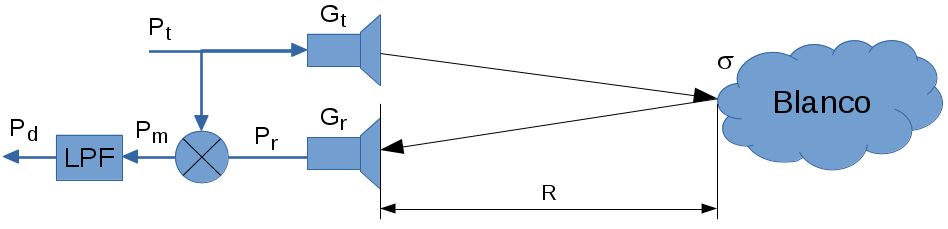
\includegraphics[width=10cm]{targetMeasurement}
 \caption{Análisis de la potencia de la señal.}
 \label{fig:powerAnalysis}
\end{figure}

Cuando el radar transmite una potencia $P_t$ y si fuese un radiador isotrópico, la densidad de potencia incidente en un cuerpo a una distancia R es igual a $P_t$ dividido el área unitaria,
\begin{equation}
  p_i = \dfrac{P_t}{4\pi R^2} \,[\si{Wm^{-2}}]
\end{equation}

Cuando el radiador no es isotrópico y el radar utiliza una antena que concentra la potencia en una dirección en particular, la densidad de potencia incidente resulta
\begin{equation}
  p_i = \dfrac{P_tG_t}{4\pi R^2} \,[\si{Wm^{-2}}]
\end{equation}

donde $G_t$ es la ganancia de la antena transmisora, definida como la relación entre densidades de potencia en la dirección en particular con respecto a un radiador isotrópico \cite{Richards2009}. Ahora, si se asume que el blanco posee un Radar Cross Section (RCS) igual a $\sigma \,[\si{m^2}]$, la potencia disponible para ser nuevamente irradiada en el blanco es 
\begin{equation}
  p_\sigma = p_i\sigma = \dfrac{P_tG_t\sigma}{4\pi R^2} \,[\si{W}]
\end{equation}

A su vez, si se asume que el blanco irradia isotrópicamente, la densidad de potencia en la antena receptora es 
\begin{equation} \label{eq:receivedDensity}
  p_r = \dfrac{P_tG_t\sigma}{(4\pi)^2 R^4} \,[\si{Wm^{-2}}]
\end{equation}

La potencia recibida es la densidad multiplicada por la apertura de la antena $A_r$, que también tiene dimensiones de área. La cual está relacionada con la ganancia de recepción por 
\begin{equation} \label{eq:receptionGain}
  G_r = \dfrac{4\pi A_r}{\lambda^2}
\end{equation}

Por lo tanto, utilizando la ecuación \ref{eq:receivedDensity} con \ref{eq:receptionGain}, la potencia recibida $P_r$ por el radar es igual a
\begin{equation}
  P_r = \dfrac{P_tG_tG_r\lambda^2\sigma}{(4\pi)^3 R^4} \,[\si{W}]
\end{equation}

La señal recibida es mezclada con la señal transmita y, si se asume un mezclador ideal, la potencia de salida $P_m$ es la multiplicación de las potencias de entrada, por lo tanto
\begin{equation}
  P_m = P_tP_r = \dfrac{P_t^2G_tG_r\lambda^2\sigma}{(4\pi)^3 R^4} \,[\si{W}]
\end{equation}

Por último, la señal mezclada es filtrada eliminando los componentes de alta frecuencia, asumiendo un filtro ideal y observando que en la ecuación \ref{eq:signalFrequency4} se elimina el término correspondiente a la suma de frecuencias, se puede deducir que la potencia de salida es la mitad que la de entrada.
\begin{equation} \label{eq:derampedPower}
  P_d = \dfrac{P_m}{2} = \dfrac{P_t^2G_tG_r\lambda^2\sigma}{2(4\pi)^3 R^4} \,[\si{W}]
\end{equation}

Ahora que se posee la relación entre la potencia de la señal a procesar y la ganancia del blanco (ecuación \ref{eq:derampedPower}), se puede determinar la relación de amplitud
\begin{equation}
  \sigma = \dfrac{2P_d(4\pi)^3 R^4}{P_t^2G_tG_r\lambda^2} \,[\si{m^2}]
\end{equation}


\section{Resumen}

En este capítulo se introdujeron los conceptos básicos sobre los dos grandes grupos de radares, los cuales son pulsados o continuos y se menciona la problemática de ambigüedades en rango asociada a cada uno de ellos. En la problemática a resolver se opta por la utilización de radares continuos a causa de la cercanía entre el blanco y el radar.

Con respecto a las antenas, se menciona una lista de los distintos tipos con descripciones y usos. Se detallan los monopolos y dipolos dado que es el tipo de antena utilizado por su simpleza de construcción. A su vez, se introduce el concepto de parámetros S y de polarización vertical y horizontal dado que las antenas utilizadas son del tipo polarimétricas y se las caracteriza midiendo dichos parámetros.

Por último, se resumen los principales tipos de modulaciones utilizados en un radar continuo detallando el diente de sierra. Asimismo, se describe el desarrollo matemático para la determinación de la distancia entre el objeto y el radar. Esto es necesario dado que la misma es utilizada para poder determinar tanto la fase como la ganancia que el blanco induce sobre la señal. Dichas perturbaciones son las variables que determinan los parámetros de dispersión.

\begin{description}

\item[Distancia entre el blanco y el radar]
Dicha variable está determinada por
\begin{equation}
  R = \dfrac{T\Delta fc}{2B\varepsilon_r} \pm \dfrac{c}{2B\sqrt{\varepsilon_r}p}
\end{equation}
donde $c$ es la velocidad de la luz, $\varepsilon_r$ es la permitividad relativa del medio, $B$ es el ancho de banda de la señal, $\Delta f$ es la diferencia de frecuencia instantánea entre la señal transmitida y recibida, $T$ es el tiempo en que es barrido el BW, desde la frecuencia mínima a la máxima y $p$ es la relación entre la frecuencia de muestreo de la señal y la cantidad de muestras utilizada para realizar la FFT.

\item[Atenuación que el blanco induce sobre la señal]
Dicha variable está determinada por
\begin{equation}
  \sigma = \dfrac{2P_d(4\pi)^3 R^4}{P_t^2G_tG_r\lambda^2}
\end{equation}
donde $P_d$ es la potencia de la señal a procesar, $P_t$ es la potencia transmitida del radar, $G_t$ es la ganancia de la antena transmisora y $G_r$ es la ganancia de la antena receptora.

\item[Desfase que el blanco induce sobre la señal]
Dicha variable está determinada por
\begin{equation}
  \theta = \dfrac{4\pi f_0R}{c} - \dfrac{2\pi BR}{c} - \dfrac{4\pi BR^2}{Tc^2} - \varphi_d
\end{equation}
donde $f_0$ es la frecuencia central de la señal transmitida y $\varphi_d$ es la fase de de la señal recibida.

Para utilizar la ecuación anterior, es fundamental que la diferencia de fase entre dos pulsos consecutivos en frecuencia sea menor que $2\pi$. Para ello, se realiza zero padding en la señal previo al cálculo de la FFT.
\end{description}
% \chapter{Desarrollo del Hardware} \label{ch:development}

% **************************** Define Graphics Path **************************
\ifpdf
    \graphicspath{{Chapter3/Figs/Raster/}{Chapter3/Figs/PDF/}{Chapter3/Figs/}}
\else
    \graphicspath{{Chapter3/Figs/Vector/}{Chapter3/Figs/}}
\fi

En este capítulo se presenta el desarrollo físico del dispositivo en función de las bases teóricas y los requerimientos definidos en el capítulo previo. El mismo se encuentra dividido en dos secciones. En la primera se explica que criterios fueron tomados en cuenta y que componentes se utilizaron para la construcción de cada sección del radar. En la segunda, se muestran las mediciones realizadas para caracterizar los distintos módulos que lo integran.


\section{Construcción}

En la figura \ref{fig:radarDiagram} se puede observar un diagrama en bloques mostrando los distintos módulos que integran el radar construido. Las siguientes secciones del capítulo explican cada uno de estos módulos por separado, salvo el procesador que se explicará en el capítulo \ref{sc:radarProcessor}.
\begin{figure}
 \centering
 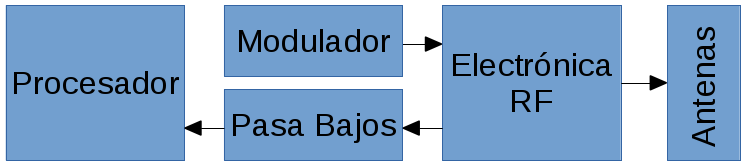
\includegraphics[width=10cm]{radarScheme}
 \caption{Diagrama en bloques básico del radar FMCW a construir.}
 \label{fig:radarDiagram}
\end{figure}


\subsection{Modulador}

Como se mencionó en la sección \ref{sc:ambiguity}, para evitar ambigüedades en la determinación del rango de medición la duración de la chirp transmitida debe ser mayor que el tiempo de ida y vuelta al blanco más alejado detectable por el radar. Como se desea una distancia máxima igual a $\SI{20}{\meter}$ (ver requerimiento \ref{req:l0}), siguiendo la relación de la ecuación \ref{eq:relDist}, se puede determinar el mínimo valor admitido de dicho período.
\begin{equation}
  \tau = \dfrac{2R\sqrt{\varepsilon_r}}{c} \approx \SI{133.43}{\nano\second}
\end{equation}

A su vez, en la sección \ref{sc:ambiguity} también se mencionó que para disminuir errores en el cálculo de la estimación en la frecuencia, se busca que el período de la señal transmitida sea al menos dos órdenes mayor que el máximo tiempo de ida y vuelta. Por lo tanto, el mínimo período resulta igual a $\SI{13.343}{\mu\second}$. De esta forma se desprende el requerimiento \ref{req:l2_pulseT}.

Las especificaciones del modulador utilizado en todos los ensayos están definidos en la tabla \ref{tab:modulatorsSpecification}. Las mismas definen los requerimientos \ref{req:l2_mod} y \ref{req:l2_dutyCycle}.

\begin{table}[htb]
  \caption{Especificaciones del modulador.}
  \centering
  \label{tab:modulatorsSpecification}
  \begin{tabular}{l c}
  \toprule
  \textbf{Característica} & \textbf{Especificación} \tabularnewline
  \midrule

  Modulación & Triangular, Senoidal \tabularnewline

  $V_{pp}$ & $\SI{5}{V}$ \tabularnewline

  Período & $\SI{14.8}{\milli\second}$ \tabularnewline

  Duty Cycle & $\SIrange[range-phrase = \rightarrow]{0.05}{99.995}{\percent}$ \tabularnewline

  \bottomrule
  \end{tabular}
\end{table}

El circuito integrado utilizado para armar el modulador, con las especificaciones mencionadas en la tabla \ref{tab:modulatorsSpecification}, es el XR-2206. Se trata de un generador de señales y su hoja de datos está especificada en \cite{Generator1972}. Dentro del mismo están los circuitos de una señal triangular, cuadrada, diente de sierra, entre otros.

En este trabajo se diseñó un circuito que, según la posición de jumpers, se modifica el tipo de señal generada. De esta forma se cumple el requerimiento \ref{req:l2_mod}. La imagen \ref{fig:schematicModulator} muestra el esquemático del circuito y la figura \ref{fig:pcbModulator} muestra el pcb. Se puede observar que el circuito posee dos llaves, $S_1$ y $S_2$, el primero es para elegir la señal de salida, sinusoidal o triangular y el segundo es para modificar el ciclo de trabajo. Para el caso sin ciclo de trabajo, la frecuencia de salida depende de la siguiente ecuación,
\begin{equation}
  f = \dfrac{1}{R_1C}
\end{equation}
en cambio, para el otro caso, 
\begin{equation}
  f = \dfrac{2}{(R_1 + R_2)C}
\end{equation}
y el ciclo de trabajo es
\begin{equation}
  \Delta T = \dfrac{R_1}{R_1 + R_2}
\end{equation}
\begin{figure}[H]
  \centering
  \begin{subfigure}[b]{0.65\textwidth}
    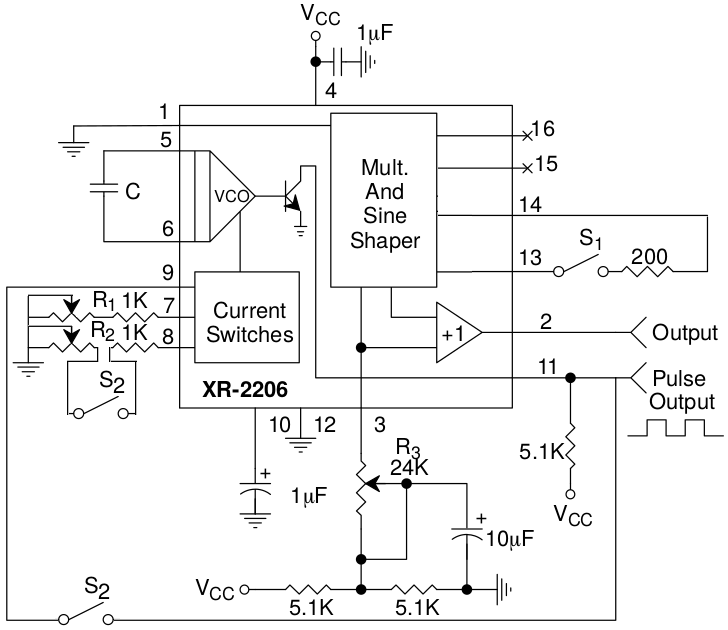
\includegraphics[width=9.5cm]{modulator}
    \caption{Esquemático del modulador.}
    \label{fig:schematicModulator} 
  \end{subfigure}

  \begin{subfigure}[b]{0.65\textwidth}
    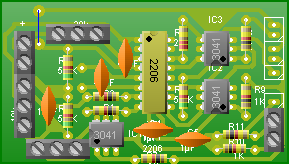
\includegraphics[width=9.5cm]{pcbModulator}
    \caption{PCB del modulador.}
    \label{fig:pcbModulator}
  \end{subfigure}

  \begin{subfigure}[b]{0.65\textwidth}
    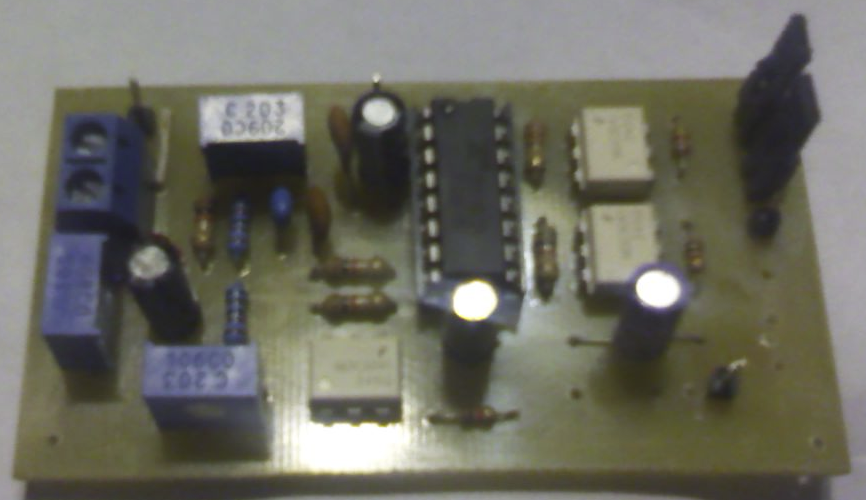
\includegraphics[width=9.5cm]{realModulator}
    \caption{Circuito construido del modulador.}
  \end{subfigure}
  \caption{Distintas etapas en la construcción del Modulador del radar.}
\end{figure}


\subsection{Electrónica de RF}

Se decidió utilizar como base la electrónica RF de un radar FMCW de banda S de baja potencia diseñado por el Instituto de Tecnología de Massachusetts (MIT). La cual posee una potencia de transmisión igual a $\SI{12}{\dBm}$. Con esto se define el requerimiento \ref{req:l2_txPower}.

La cadena está compuesta por un generador controlado por tensión (VCO), atenuadores, divisores de potencia, amplificadores y un mezclador, ver figura \ref{fig:rfElectronics}. A continuación se describen las principales características de cada uno de los componentes mencionados.

\begin{figure}[htb]
  \centering
  \begin{subfigure}{\textwidth}
    \centering
    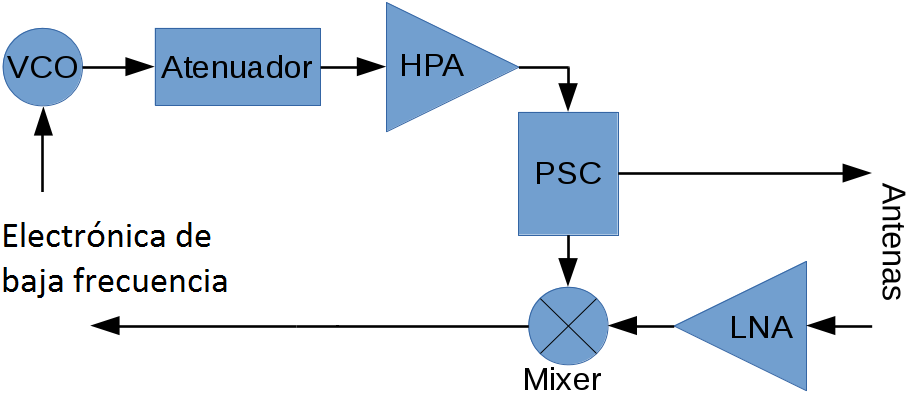
\includegraphics[width=10cm]{rfElectronics}
    \caption{Circuito esquemático}
  \end{subfigure}

  \begin{subfigure}{\textwidth}
    \centering
    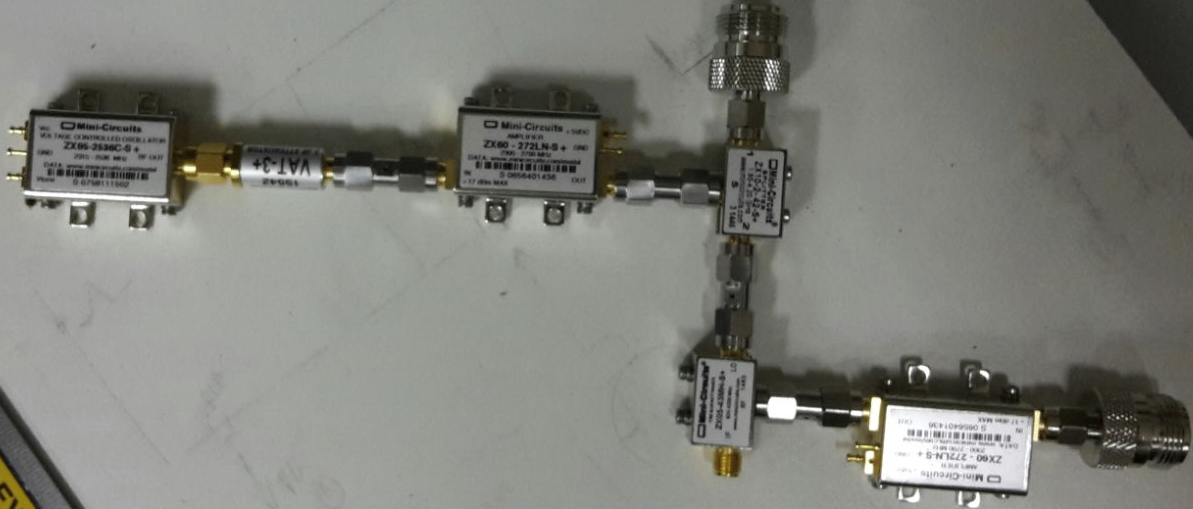
\includegraphics[width=10cm]{rfElectronics2}
    \caption{Electrónica de RF armada.}
  \end{subfigure}
  \caption{Distintas etapas en la construcción de la electrónica de RF.}
  \label{fig:rfElectronics}
\end{figure}

\begin{description}
  \item[VCO] El código de dicho componente es ZX95-2536C \cite{VCOMiniCircuits}. La frecuencia de la señal transmitida depende de la tensión de entrada, dicha dependencia puede observarse en la figura \ref{fig:freqVsVoltage}. La potencia transmitida es de $\SI{6.2}{\dBm}$ cuando la tensión de alimentación es de $\SI{5}{V}$. La frecuencia central de trabajo es igual a $\SI{2450}{\MHz}$ y posee un ancho de banda de transmisión máximo igual a $\SI{300}{\MHz}$. De esta forma se definen los requerimientos \ref{req:l2_f0} y \ref{req:l2_bw}.
  \begin{figure}[H]
   \centering
   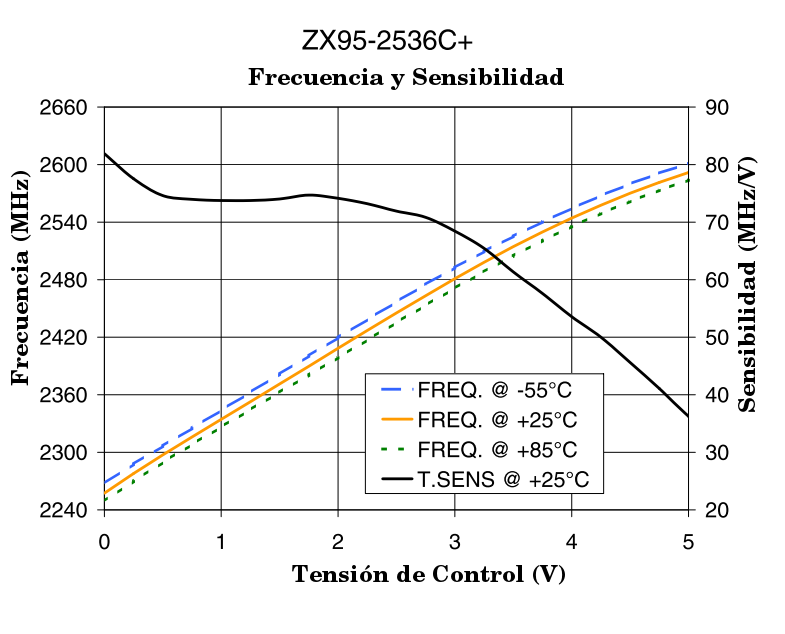
\includegraphics[width=10cm]{frequencyVsVoltage}
   \caption{Frecuencia generada en función de la tensión de control \cite{VCOMiniCircuits}.}
   \label{fig:freqVsVoltage}
  \end{figure}
  
  \item[Atenuador] El código de dicho componente es VAT-3 \cite{AttMiniCircuits}. En la frecuencia de trabajo del VCO, la señal es atenuada en $\SI{3.2}{\deci\bel}$. El mismo es utilizado para proteger al generador ante cualquier señal reflejada por desadaptaciones o por mal conexionado del instrumental.

  \item[Divisor de potencia] El código de dicho componente es ZX10-2-42 \cite{PSCMiniCircuits}. El mismo posee una pérdida por inserción desde el puerto central a los individuales igual a $\SI{3.26}{\dB}$ en una frecuencia de $\SI{2460}{\MHz}$. La figura \ref{fig:insertionLoss} muestra dicha pérdida en función de la frecuencia de trabajo.

  \begin{figure}[H]
   \centering
   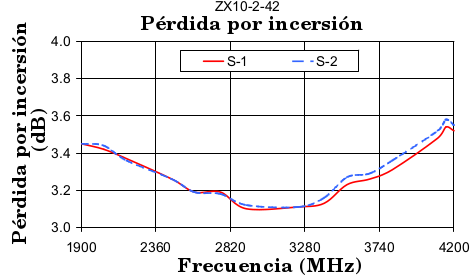
\includegraphics[width=10cm]{insertionLoss}
   \caption{Pérdida de inserción en el divisor de potencia \cite{PSCMiniCircuits}.}
   \label{fig:insertionLoss}
  \end{figure}

  \item[Amplificador] El código de dicho componente es ZX60-272LN \cite{LNAMiniCircuits}. Según la hoja de datos, el mismo posee una ganancia igual a $\SI{14}{\deci\bel}$ para la frecuencia central de trabajo del VCO.

  \item[Mezclador] El código de dicho componente es ZX05-43MH \cite{mixerMiniCircuits}. Según la hoja de datos, el mismo posee una pérdida por conversión igual a $\SI{5.5}{\deci\bel}$ para la frecuencia central de trabajo del VCO.

\end{description}


\subsection{Antenas}

Las antenas escogidas son del tipo apertura dado que se requiere cierta direccionalidad. A su vez, se decide utilizar una para transmitir y otra para recibir. Por cada cavidad hay dos monopolos distribuidos de forma ortogonal entre sí para poder transmitir y recibir en ambas polarizaciones, horizontal (H) y vertical (V). De esta forma se definen los requerimientos \ref{req:l2_antQuantity}, \ref{req:l2_antenna} y \ref{req:l2_polarization}. Los atributos a definir son la altura de la pesca, la distancia de la misma a la pared de la cavidad, la longitud y diámetro del caño. Los mismos dependen de la frecuencia de trabajo y el modo en que se desee trabajar.

\begin{figure}
 \centering
 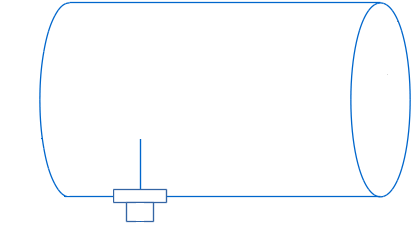
\includegraphics[width=8cm]{antennas}
 \caption{Dimensiones de una guía de onda de medio tubo.}
 \label{fig:antennas}
\end{figure}

Cada modo de resonancia es definido por una frecuencia de corte inferior, el cual no podría existir a frecuencias inferiores. El modo dominante es el que posee la menor frecuencia de corte posible. Para este tipo de guías de ondas es el TE$_{11}$. En este modo no hay campo eléctrico en la dirección de la propagación de la onda y define la relación entre el radio de la antena, $R$, y la frecuencia de corte \cite{circularWaveguides}.
\begin{equation} \label{eq:freqInf}
  f_c = \dfrac{\num{1.8412}}{2\pi R} c
\end{equation}

La longitud de onda dentro de la guía es mayor a la de la señal en espacio libre y responde a la siguiente ecuación,
\begin{equation} \label{eq:lambdaInGuide}
\lambda_g = \begin{cases} \dfrac{\lambda}{\sqrt{1 - (\dfrac{f_c}{f})^2}}, & \mbox{donde } f > f_c \\ \infty, & \mbox{donde } f = f_c \end{cases}
\end{equation}

Se debe elegir el tamaño de la guía de forma tal que el ancho de banda de operación entre completamente dentro de dicho modo de de resonancia, por lo tanto la máxima frecuencia de trabajo debe ser menor a la frecuencia de corte de TE$_{21}$ \cite{circularWaveguides},
\begin{equation} \label{eq:freqSup}
  f_{csup} = \dfrac{\num{3.0542}c}{2\pi R}
\end{equation}

\begin{description}
  \item[Altura de la pesca] Este atributo se corresponde con el requerimiento \ref{req:l2_pescaLength} y se define como la cuarta parte de la longitud de onda de la señal transmitida en espacio libre. En este caso se utiliza la frecuencia central de trabajo.

  \begin{equation}
  WireLength = \dfrac{\lambda}{4}
  \end{equation}

Dado que la frecuencia de trabajo utilizada es igual a $\SI{2450}{\MHz}$, la longitud de la pesca resulta aproximadamente igual a $\SI{3}{\centi\meter}$.

  \item[Longitud y diámetro de la guía de onda circular] Estos atributos se corresponden con el requerimiento \ref{req:l2_cavity}. Como se mencionó previamente, las frecuencias de cortes inferiores de cada modo de resonancia depende del diámetro de la guía de ondas, por lo tanto el ancho de banda de cada modo se encuentra determinado por las mismas. Y como se desea que las frecuencias de trabajo, $\SI{2300}{\MHz} - \SI{2600}{\MHz}$, entren dentro del modo dominante, el diámetro máximo y mínimo admisible es de,
  \begin{equation}
  \SI{7.64}{\centi\meter} < D < \SI{11.2}{\centi\meter}
  \end{equation}

  El resultado anterior fue obtenido siguiendo las ecuaciones \ref{eq:freqInf} y \ref{eq:freqSup}. La antena que se consiguió posee una longitud igual a $\SI{15}{\centi\meter}$ y un diámetro igual a $\SI{10}{\centi\meter}$, por lo tanto, el ancho de banda admisible del modo dominante es de $\SI{1157.5}{\MHz}$ con una frecuencia central de $\SI{2335.75}{\MHz}$.

  \item[Distancia monopolo a la pared de la guía de onda] Este atributo se corresponde con el requerimiento \ref{req:l2_cavityDistance}. Dado que la guía de onda es cilíndrica y que el monopolo transmite omnidireccionalmente en el plano perpendicular al mismo \cite{arrl2007}, parte de la onda se transmite hacia el frente de la guía pero otra parte hacia el fondo, la misma se refleja con la pared metálica volviendo al punto de origen con dirección del frente de la antena.

  Para que la interferencia de ondas sea constructiva, es necesario que el eco posea la misma fase que la señal a transmitir. Se logra el efecto deseado si la separación entre el monopolo y la pared es de $\frac{\lambda}{4}$, dado que el eco en un medio metálico implica un desfase de $\SI{180}{\degree}$. Siguiendo la ecuación \ref{eq:lambdaInGuide}, y dado que la frecuencia central de trabajo es de $\SI{2450}{\MHz}$, la longitud de onda dentro de la guía de onda es igual a $\SI{17.56}{\centi\meter}$, por lo tanto la distancia resultante es $\SI{4.39}{\centi\meter}$.

\end{description}

\subsection{Pasa Bajos}

El circuito pasa bajos del receptor, utilizado para filtrar todas las frecuencias salvo las pertenecientes al rango de trabajo del radar, es el sallen-key \cite{Unwin2003}. Este circuito, ilustrado en la figura \ref{fig:lowPassCircuit}, consta de tres etapas. La primera es un amplificador no inversor y las siguientes son pasa bajos de segundo orden con una frecuencia de corte del orden de $\SI{20}{\kHz}$, conformando un circuito de cuarto orden con una frecuencia de corte igual a los $\SI{20}{\kHz}$, definiéndose así el requerimiento \ref{req:l2_filter}. Dicho valor surge de que la señal, luego de ser filtrada, se recibe en la computadora a través del jack del micrófono, el cual posee una frecuencia de muestreo de $\SI{40}{\kHz}$. Por lo tanto, para cumplir con el teorema de nyquist, si se desea evitar el aliasing en la señal, la frecuencia máxima no puede superar $\SI{20}{\kHz}$.

Cabe destacar que, como el radar trabaja con tensiones de $\SI{12}{\volt}$ y $\SI{5}{\volt}$, los amplificadores están alimentados con la tensión de mayor denominación y las resistencias conectadas a sus pines inversores con la tensión de menor denominación.

\begin{figure}
 \centering
 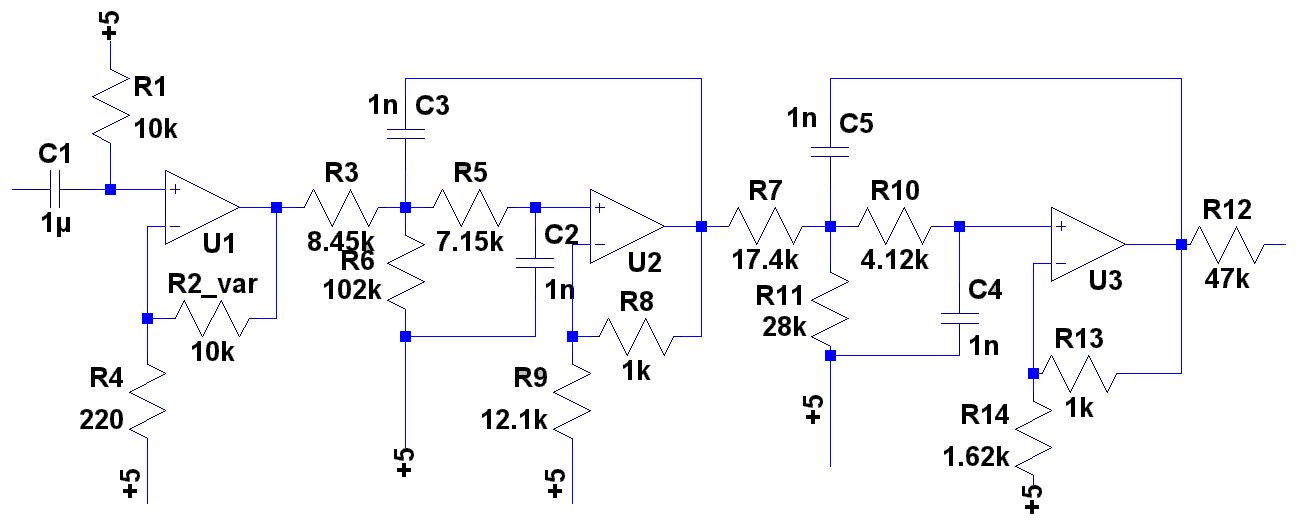
\includegraphics[width=15cm]{lowPassBand}
 \caption{Circuito pasa bajos y amplificador de señal.}
 \label{fig:lowPassCircuit}
\end{figure}

La entrada al circuito amplificador posee un capacitor en serie para eliminar el offset de la señal de entrada y una resistencia conectada a los $\SI{5}{\volt}$ estableciendo el offset común. La existencia del capacitor en serie a la señal resulta en un circuito pasa altos, con una frecuencia de corte inferior igual a
\begin{equation}\label{eq:fcInf}
  fc = \dfrac{1}{2\pi R_1 C_1} = \SI{7.23}{\Hz}
\end{equation}

La ecuación \ref{eq:gainAmplifier} es la transferencia de este circuito para cuando se considera despreciable la influencia del capacitor serie sobre la señal.
\begin{equation}\label{eq:gainAmplifier}
  Av = 1 + \dfrac{R_2}{R_4}
\end{equation}

Las siguientes etapas fueron caracterizadas utilizando las ecuaciones que definen al filtro sallen-key, listadas en la referencia \cite{Unwin2003}. Pero, como dichos circuitos no son exactamente iguales por la existencia de las resistencias $R_6$ y $R_{11}$ de la figura \ref{fig:lowPassCircuit}, dichas ecuaciones no pueden ser utilizadas directamente. Si se realiza un corte en cada etapa, como se muestra en la figura \ref{fig:genericSallen}, para calcular el equivalente de thevenin, se obtiene el circuito mostrado en la figura \ref{fig:genericSallen2}.

\begin{figure}
  \centering
  \begin{subfigure}{0.4\textwidth}
    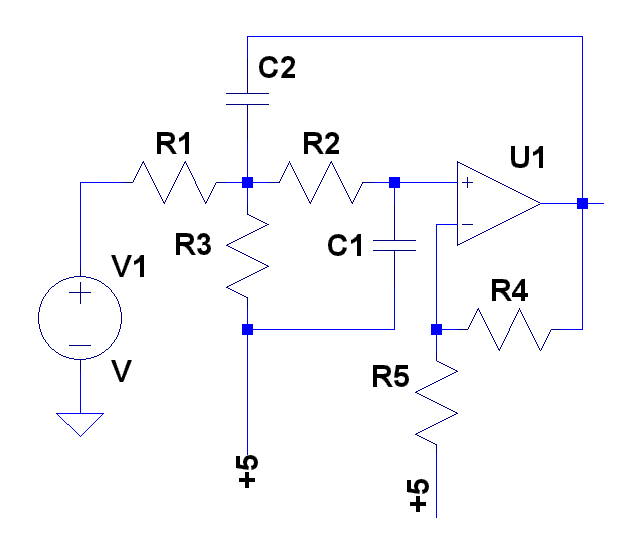
\includegraphics[width=6cm]{genericSallenKey}
    \caption{Etapa generica del circuito pasa bajo del radar}
    \label{fig:genericSallen}   
  \end{subfigure}
  {\color{blue}\LARGE$\Rightarrow$}
  \begin{subfigure}{0.4\textwidth}
    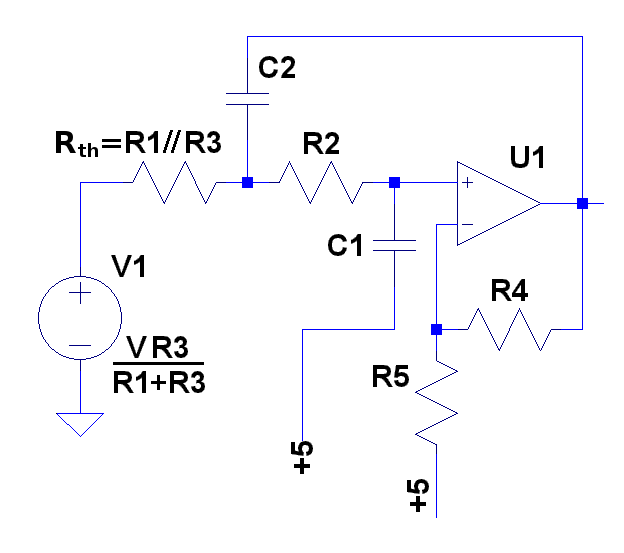
\includegraphics[width=6cm]{genericSallenKey2}
    \caption{Equivalente del circuito pasa bajos del radar}
    \label{fig:genericSallen2}
  \end{subfigure}             
  \caption{Equivalente filtro Sallen-key}
\end{figure}
Manteniendo la nomenclatura de los componentes mostrados en la figura \ref{fig:genericSallen2}, las ecuaciones para calcular la ganancia a bajas frecuencias, la frecuencia de corte y el Q de cada etapa son \ref{eq:gainLowPass}, \ref{eq:f0LowPass} y \ref{eq:qLowPass} respectivamente.
\begin{equation}\label{eq:gainLowPass}
  Av = 1 + \dfrac{R_4}{R_5}
\end{equation}
\begin{equation}\label{eq:f0LowPass}
  f_0 = \dfrac{1}{2\pi\sqrt{R_{th}R_2C_1C_2}}
\end{equation}
\begin{equation}\label{eq:qLowPass}
  Q = \dfrac{\sqrt{R_{th}R_2C_1C_2}}{R_{th}C_1 + R_2C_1 + \dfrac{R_{th}C_2R_4}{R_5}}
\end{equation}

La tabla \ref{tab:lowPassProperties} resume la ganancia y frecuencias de corte y Q de cada etapa.

\begin{table}[htb]
  \caption{Propiedades de las etapas del filtro del receptor.}
  \centering
  \label{tab:lowPassProperties}
  \begin{tabular}{l c c c}
  \toprule
  \textbf{Etapa} & \textbf{Ganancia} & \textbf{Frecuencia Corte} & \textbf{Q} \tabularnewline
   & [veces] & [Hz] & \tabularnewline
  \midrule
  Primera & 1 - 46,45 & - & - \tabularnewline

  segunda & 1,08 & 21306 & 0,52 \tabularnewline

  tercera & 1,62 & 23935 & 0,8 \tabularnewline

  \bottomrule
  \end{tabular}
\end{table}

Las imágenes de la figura \ref{fig:lowPassFilterCircuit} muestran el PCB y el circuito pasa bajos armado.
\begin{figure}[H]
  \centering
  \begin{subfigure}[b]{0.47\textwidth}
    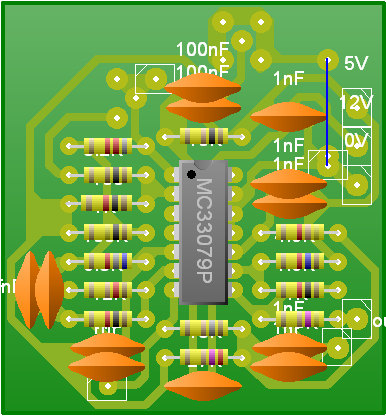
\includegraphics[width=7cm]{pcbLPF}
    \caption{PCB del filtro pasa bajos.}
  \end{subfigure}
  \begin{subfigure}[b]{0.47\textwidth}
    \includegraphics[width=7cm]{lowPassFilter}
    \caption{Circuito construido del filtro pasa bajos.}
  \end{subfigure}
  \caption{Distintas etapas en la construcción del filtro pasa bajos del radar.}
  \label{fig:lowPassFilterCircuit}
\end{figure}


\subsection{Procesador}

Dado que el procesador es software, se lo detallará junto al simulador en el capítulo \ref{ch:softwareDevelopment}.

\subsection{Gabinete}

El hecho de querer montar en un futuro al radar en un dron introduce ciertos requerimientos de volumen y peso que afectan en la decisión del gabinete a utilizar, como el que no debe pesar más de $\SI{1}{\kg}$. Dado que se requiere que sea lo más liviano posible y en un volumen determinado, se optó por utilizar plástico como material. El compuesto del mismo es poliestireno de alto impacto y es fabricado con la técnica de termoformado. El peso final del radar resulta ser de $\SI{600}{\gram}$ cumpliéndose el requerimiento \ref{req:l2_weight}.

Como habrán otros componentes electrónicos que pueden afectar al funcionamiento del radar por interferencia electromagnéticas (EMI), se debe metalizar el gabinete. Una de las posibles estrategias es la del metalizado al vacío, aunque dicho proceso quedará como trabajo futuro.

La figura \ref{fig:radar3D} muestran la modelización del radar completo, como se vería el interior como el exterior del mismo.
\begin{figure}[H]
 \centering
 \begin{subfigure}[t]{0.49\textwidth}
    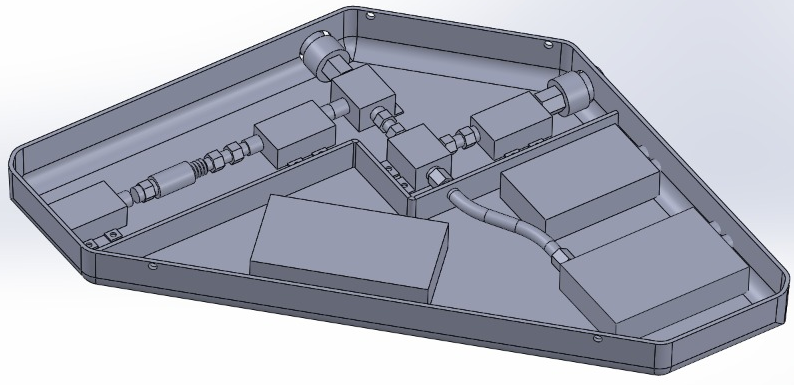
\includegraphics[width=7.5cm]{radar3D}
  \end{subfigure}
  \begin{subfigure}[t]{0.49\textwidth}
    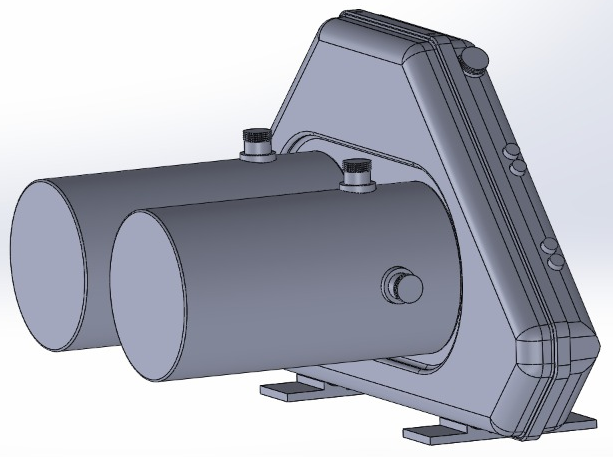
\includegraphics[width=7.5cm]{completeRadar}
  \end{subfigure}
 \caption{Modelo del gabinete interna y exterma.}
 \label{fig:radar3D}
\end{figure}

La figura \ref{fig:completeRadar} muestra tanto el interior del gabinete armado con la distribución de los componentes dentro del mismo como el radar de perfil.

\begin{figure}[H]
 \centering
 \begin{subfigure}[t]{0.8\textwidth}
    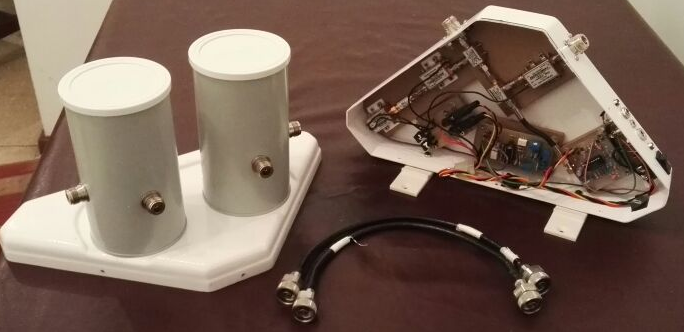
\includegraphics[width=12cm]{openedRuiltRadar}
  \end{subfigure}

  \begin{subfigure}[t]{0.5\textwidth}
    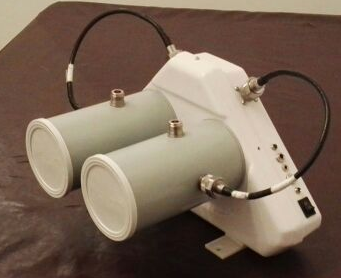
\includegraphics[width=7.5cm]{completeBuiltRadar}
  \end{subfigure}
 \caption{Modelo del gabinete interna y externa.}
 \label{fig:completeRadar}
\end{figure}


\section{Mediciones de funcionamiento}

En esta sección se muestran distintas mediciones sobre diversos módulos del radar para caracterizarlo.
Los instrumentos utilizados son
\begin{itemize}
  \item Analizador de espectros: Rhode \& Schwartz ESU 40 \cite{spectrumAnalyzer}.
  \item Analizador de redes Vectorial (VNA): Keysight Technologies N9923A FieldFox RF.
Vector Network Analyzer \cite{VNA}.
  \item Osciloscopio: Goodwill, GOS-653G
  \item Contador: GoodWill, GUC-2020
  \item Generador de señales: Topward, FG-8140
\end{itemize}

\subsection{Transferencia, filtro pasa bajos}

Para la medición de la función de transferencia del filtro se utilizó un generador de señales, un osciloscopio y un contador. Al primero se lo conectó a la entrada del circuito. Al resto del instrumental se lo conectó tanto a la entrada como a la salida del mismo. La figura \ref{fig:lowPassFilterConnections} muestra el banco de trabajo utilizado para realizar la medición.

\begin{figure}[H]
 \centering
 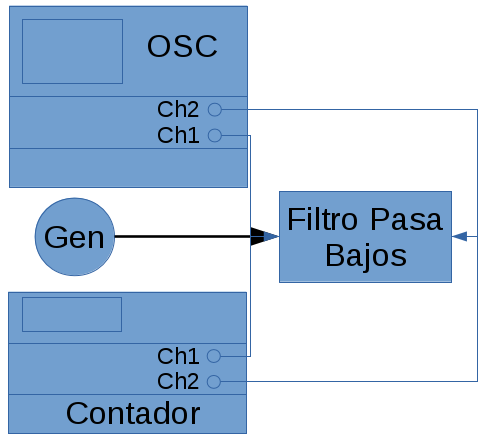
\includegraphics[width=6cm]{lowPassFilterTransferenceWorkbench}
 \caption{Banco de medición, transferencia del filtro pasa bajos.}
 \label{fig:lowPassFilterConnections}
\end{figure}

Durante el ensayo se midió tanto la tensión de entrada como la de salida con el osciloscopio a medida que se fue variando la frecuencia del generador para determinar la ganancia del circuito. A su vez, con el contador se determinó el desfase entre ambas señales midiendo el intervalo de tiempo entre los flancos ascendentes de cada una. La tabla \ref{tab:lowPassFilterTransference} y la figura \ref{fig:lowPassFilterTransference} muestran los resultados obtenidos.

La incertidumbre de las mediciones de tensiones medidas es del $\SI{3}{\percent}$. Por lo tanto la incertidumbre de la ganancia es del $\SI{6}{\percent}$. En cambio, la incertidumbre del intervalo de tiempo y el de la frecuencia ronda el $\SI{1}{\percent}$ dado que el instrumento fue configurado para disminuir la incertidumbre asociada a la medición. Por lo tanto la incertidumbre del desfase es del $\SI{2}{\percent}$. La tabla \ref{tab:lowPassFilterTransference} y la figura \ref{fig:lowPassFilterTransference} muestran los resultados obtenidos.

En la figura \ref{fig:lowPassFilterTransference} se muestran dos curvas, en rojo la ganancia y en azul la fase en función de la frecuencia. Se puede observar que el ancho de banda del circuito es aproximadamente de $\SI{20}{\kHz}$ con una frecuencia de corte inferior igual a $\SI{10}{\Hz}$. Es importante notar que la misma es plana hasta una frecuencia de $\SI{10}{\kHz}$. En cambio, observando el desfase del circuito, el mismo es igual a $\SI{0}{\degree}$ en un rango de frecuencias de $\SI{30}{\Hz}$ a $\SI{2}{\kHz}$. Si la señal recibida se encuentra en otros valores de frecuencias, habría que substraer el efecto de este subsistema sobre la misma para eliminar el error sistemático. De esta forma se verifica el requerimiento \ref{req:l2_filter}.

\begin{table}[H]
  \caption{Transferencia del circuito pasa bajos.}
  \centering
  \label{tab:lowPassFilterTransference}
  \begin{tabular}{S[table-auto-round, table-format=5.2] *{2}{S[table-auto-round, table-format=1.2]} S[table-auto-round, table-format=-4.2] S[table-auto-round, table-format=2.1] S[table-auto-round, table-format=-3]}
  \toprule
  
  {\textbf{Frec}} & \textbf{Vin} & \textbf{Vout} & \textbf{Intervalo de T} & \textbf{Ganancia} & \textbf{Desfase} \tabularnewline
  
   {[$\si{\Hz}$]} & {[$\si{\V}$]} & {[$\si{\V}$]} & {[$\si{\mu\sec}$]} & {[$\si{\dB}$]} & {[$\si{\degree}$]} \tabularnewline
  
  \midrule
  9.97 & 0.6 & 1.48 & -7462 & 7.8422093002 & 26.7826104 \tabularnewline

  20 & 0.6 & 1.95 & -905 & 10.2376672196 & 6.516 \tabularnewline

  29.37 & 0.6 & 2 & 0 & 10.4575749056 & 0 \tabularnewline

  51.11 & 0.6 & 2 & 0 & 10.4575749056 & 0 \tabularnewline

  100 & 0.6 & 2.1 & 0 & 10.881360887 & 0 \tabularnewline

  192 & 0.6 & 2.1 & 0 & 10.881360887 & 0 \tabularnewline

  305 & 0.6 & 2 & 0 & 10.4575749056 & 0 \tabularnewline

  400 & 0.6 & 2 & 13.37 & 10.4575749056 & -1.92528 \tabularnewline

  500 & 0.6 & 2 & 15.99 & 10.4575749056 & -2.8782 \tabularnewline

  600 & 0.6 & 2 & 16.45 & 10.4575749056 & -3.5532 \tabularnewline

  700 & 0.6 & 2 & 17.86 & 10.4575749056 & -4.50072 \tabularnewline

  800 & 0.6 & 2 & 18.65 & 10.4575749056 & -5.3712 \tabularnewline

  900 & 0.6 & 2 & 19.28 & 10.4575749056 & -6.24672 \tabularnewline

  1000 & 0.6 & 2 & 19.75 & 10.4575749056 & -7.11 \tabularnewline

  2000 & 0.6 & 2 & 12.48 & 10.4575749056 & -8.9856 \tabularnewline

  3000 & 0.6 & 2 & 15.8 & 10.4575749056 & -17.064 \tabularnewline

  4000 & 0.6 & 2 & 17.77 & 10.4575749056 & -25.5888 \tabularnewline

  5050 & 0.6 & 2 & 18.95 & 10.4575749056 & -34.4511 \tabularnewline

  6000 & 0.6 & 2 & 19.66 & 10.4575749056 & -42.4656 \tabularnewline

  7000 & 0.6 & 2 & 20.14 & 10.4575749056 & -50.7528 \tabularnewline

  8000 & 0.6 & 2 & 20.64 & 10.4575749056 & -59.4432 \tabularnewline

  9000 & 0.6 & 2 & 21.01 & 10.4575749056 & -68.0724 \tabularnewline

  10020 & 0.6 & 2 & 21.34 & 10.4575749056 & -76.977648 \tabularnewline

  11000 & 0.6 & 2 & 21.63 & 10.4575749056 & -85.6548 \tabularnewline

  12000 & 0.6 & 1.85 & 21.98 & 9.7804095604 & -94.9536 \tabularnewline

  13000 & 0.6 & 1.85 & 22.27 & 9.7804095604 & -104.2236 \tabularnewline

  14000 & 0.6 & 1.8 & 22.56 & 9.5424250944 & -113.7024 \tabularnewline

  15000 & 0.6 & 1.8 & 22.7 & 9.5424250944 & -122.58 \tabularnewline

  16000 & 0.6 & 1.75 & 22.92 & 9.2977359661 & -132.0192 \tabularnewline

  17000 & 0.6 & 1.7 & 23.07 & 9.0459534199 & -141.1884 \tabularnewline

  18000 & 0.6 & 1.6 & 23.29 & 8.5193746454 & -150.9192 \tabularnewline

  20000 & 0.6 & 1.44 & 23.72 & 7.6042248342 & -170.784 \tabularnewline

  26000 & 0.62 & 1 & 24.52 & 4.15216621 & -229.5072 \tabularnewline
  \bottomrule
  \end{tabular}
\end{table}

\begin{figure}[H]
 \centering
 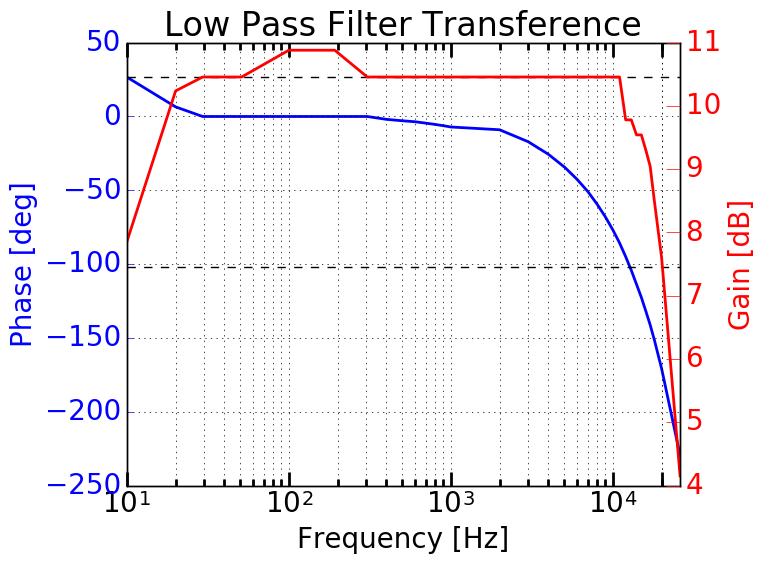
\includegraphics[width=12cm]{transference}
 \caption{Transferencia del circuito pasa bajos. En rojo la ganancia y en azul el desfase.}
 \label{fig:lowPassFilterTransference}
\end{figure}


\subsection{Potencia transmitida}

Para la medición de la potencia transmitida del radar se utilizó el analizador de espectros conectado en el cable que une la antena transmisora con el resto de la electrónica del radar. La figura \ref{fig:txPowerConnections} muestra el banco de trabajo utilizado para realizar la medición.

\begin{figure}[H]
 \centering
 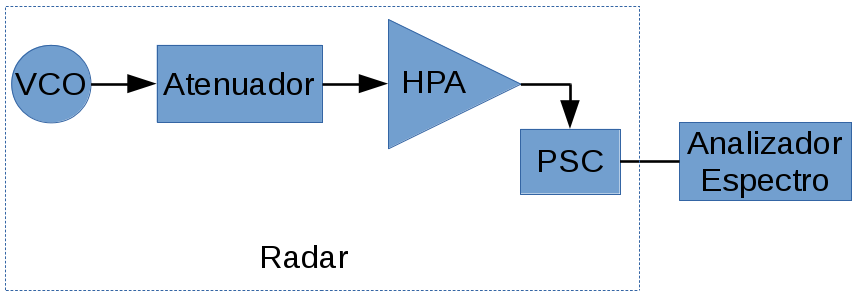
\includegraphics[width=10cm]{txPowerWorkbench}
 \caption{Banco de medición, potencia transmitida del radar.}
 \label{fig:txPowerConnections}
\end{figure}

La tabla \ref{tab:PNAConfigTxPower} resume las configuraciones utilizadas en el analizador de espectros para la medición y la figura \ref{fig:txPowerMeasurements} muestra el resultado de la medición.

\begin{table}[H]
  \caption{Configuración del analizador de espectros para medir la potencia transmitida del radar.}
  \centering
  \label{tab:PNAConfigTxPower}
  \begin{tabular}{l c c}
  \toprule
  \textbf{Característica} & \textbf{Configuración} & \textbf{Unidad} \tabularnewline
  \midrule
  Mode & ANALYZER & \tabularnewline

  Center Freq & 2434262820,514000 & \si{\hertz} \tabularnewline

  Freq Offset & 0,000000 & \si{\hertz} \tabularnewline

  Span & 1000000000,000000 & \si{\hertz} \tabularnewline

  x-Axis & LIN & \tabularnewline

  Start & 1934262820,514000 & \si{\hertz} \tabularnewline

  Stop & 2934262820,514000 & \si{\hertz} \tabularnewline

  Ref Level & 18,000000 & \si{\dBm} \tabularnewline

  Level Offset & 0,000000 & \si{\deci\bel} \tabularnewline

  Ref Position & 100,000000 & \si{\percent} \tabularnewline

  y-Axis & LOG & \tabularnewline

  Level Range & 50,000000 & \si{\deci\bel} \tabularnewline

  Rf Att & 70,000000 & \si{\deci\bel} \tabularnewline

  RBW & 10000000,000000 & \si{\hertz} \tabularnewline

  VBW & 10000000,000000 & \si{\hertz} \tabularnewline

  SWT & 0,002500 & \si{\second} \tabularnewline

  Trace Mode & CLR/WRITE & \tabularnewline

  Detector & RMS & \tabularnewline

  Sweep Count & 0 & \tabularnewline

  \bottomrule
  \end{tabular}
\end{table}

En la figura \ref{fig:txPowerMeasurements} se puede observar que la potencia transmitida por el radar es de $\SI{11.87}{\dBm}$ en una frecuencia central igual a $\SI{2.43}{\giga\hertz}$ y que el piso de ruido para esta medición se encuentra entre los $\SI{-14}{\dBm}$ y $\SI{-17.4}{\dBm}$. De esta forma se valida el requerimiento \ref{req:l2_txPower}.

\begin{figure}[H]
 \centering
 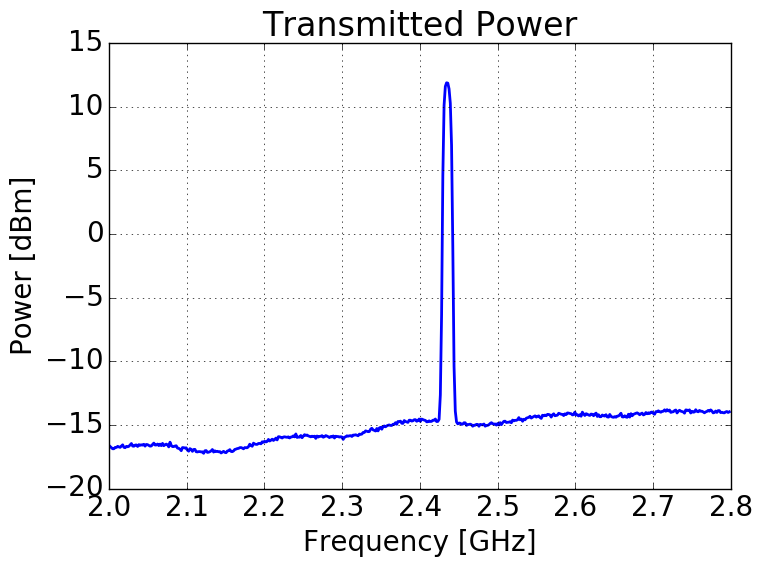
\includegraphics[width=9cm]{txPower}
 \caption{Potencia transmitida del radar medida con un PNA.}
 \label{fig:txPowerMeasurements}
\end{figure}


\subsection{Ancho de banda}

Para la medición del ancho de banda transmitido se utiliza el analizador de espectros conectado en el cable que une la antena transmisora con el resto de la electrónica del radar. La figura \ref{fig:bartPowerConnections} muestra el banco de trabajo utilizado para realizar la medición.

\begin{figure}[H]
 \centering
 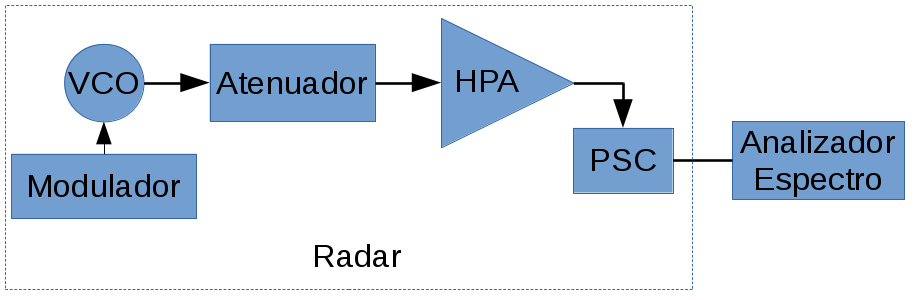
\includegraphics[width=10cm]{bartPowerWorkbench}
 \caption{Banco de medición, cabeza de chirp transmitida del radar.}
 \label{fig:bartPowerConnections}
\end{figure}

La tabla \ref{tab:PNAConfigBartPower} resume las configuraciones utilizadas en el analizador de espectros para la medición y la figura \ref{fig:bartPowerMeasurements} muestra el resultado de la medición.

\begin{table}[H]
  \caption{Configuración del analizador de espectros, medición del BW transmitido del radar.}
  \centering
  \label{tab:PNAConfigBartPower}
  \begin{tabular}{l c c}
  \toprule
  \textbf{Característica} & \textbf{Configuración} & \textbf{Unidad} \tabularnewline
  \midrule
  Mode & ANALYZER & \tabularnewline

  Center Freq & 2450288461,540000 & \si{\hertz} \tabularnewline

  Freq Offset & 0,000000 & \si{\hertz} \tabularnewline

  Span & 1000000000,000000 & \si{\hertz} \tabularnewline

  x-Axis & LIN & \tabularnewline

  Start & 1950288461,540000 & \si{\hertz} \tabularnewline

  Stop & 2950288461,540000 & \si{\hertz} \tabularnewline

  Ref Level & 18,000000 & \si{\dBm} \tabularnewline

  Level Offset & 0,000000 & \si{\deci\bel} \tabularnewline

  Ref Position & 100,000000 & \si{\percent} \tabularnewline

  y-Axis & LOG & \tabularnewline

  Level Range & 50,000000 & \si{\deci\bel} \tabularnewline

  Rf Att & 70,000000 & \si{\deci\bel} \tabularnewline

  RBW & 10000000,000000 & \si{\hertz} \tabularnewline

  VBW & 10000000,000000 & \si{\hertz} \tabularnewline

  SWT & 0,002500 & \si{\second} \tabularnewline

  Trace Mode & MAXHOLD & \tabularnewline

  Detector & RMS & \tabularnewline

  Sweep Count & 0 & \tabularnewline
  \bottomrule
  \end{tabular}
\end{table}

\begin{figure}[H]
 \centering
 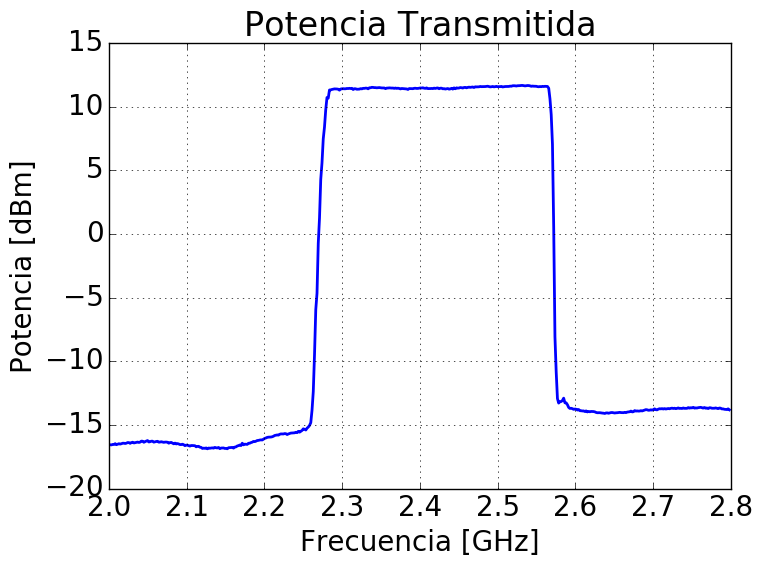
\includegraphics[width=10cm]{chripHeadPower}
 \caption{Potencia transmitida del radar medida con un analizador de espectros.}
 \label{fig:bartPowerMeasurements}
\end{figure}

Se puede observar que el ancho de banda de la señal transmitida, a $\SI{-3}{\dB}$ con respecto al pico, es igual a $\SI{291.67}{\mega\hertz}$. A su vez, la potencia de la señal es de $\SI{12}{\dBm}$ mientras que el piso de ruido es de $\SI{-15}{\dBm} \pm \SI{2}{\dBm}$. De esta forma se verifica el requerimiento \ref{req:l2_bw}.


\subsection{Parámetros S de las antenas} \label{ssc:sParameters}

Esta medición está diseñada para caracterizar el comportamiento de las antenas tanto de forma individual, midiendo el coeficiente de reflexión $S_{11}$ de cada una, como de forma grupal, midiendo el coeficiente de transmisión $S_{21}$ entre las mismas. Idealmente estos valores deberían ser 0, dado que mientras más alejado a dicho valor sea el $S_{11}$, menor es la potencia que ingresa a la antena. En cambio, el parámetro $S_{21}$ está relacionado directamente con el acoplamiento mutuo entre las antenas. Mientras mayor es dicho valor, mayor potencia recibe la antena receptora, lo cual es un efecto indeseado dado que ya se estaría recibiendo señal sin siquiera haber presencia de un blanco iluminado a caracterizar.

El banco de medición está compuesto por un VNA en donde cada canal del mismo está conectado a una antena del radar, de esta forma  la señal se transmite por una antena y se recibe a través de la segunda, ver figura \ref{fig:sParamsConnections}.
\begin{figure}[H]
 \centering
 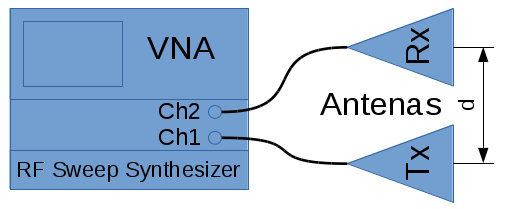
\includegraphics[width=8cm]{sParamsAntenaWorkbench}
 \caption{Banco de medición, parámetros S de las antenas.}
 \label{fig:sParamsConnections}
\end{figure}

Como las antenas son plarimétricas, se repitió la medición en todas las posibles combinaciones de polarizaciones, HH, HV, VH y VV. Es importante notar que la distancia entre los centros de las antenas permaneció invariante e igual a $\SI{15.5}{\centi\meter}$. La figura \ref{fig:sParametersMeasurements} posee los resultados de los cuatro ensayos.

\begin{figure}[H]
  \centering
  \begin{subfigure}{0.47\textwidth}
    \centering
    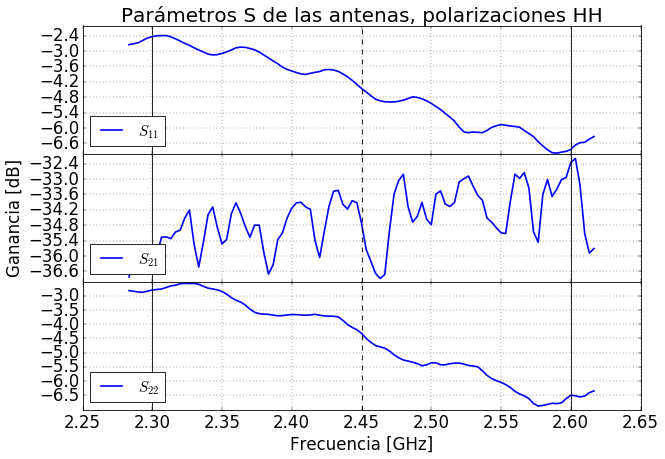
\includegraphics[width=7cm]{SParamsHH}
    \caption{Polarización HH}
    \label{subfig:hhPol}
  \end{subfigure}
  \begin{subfigure}{0.47\textwidth}
    \centering
    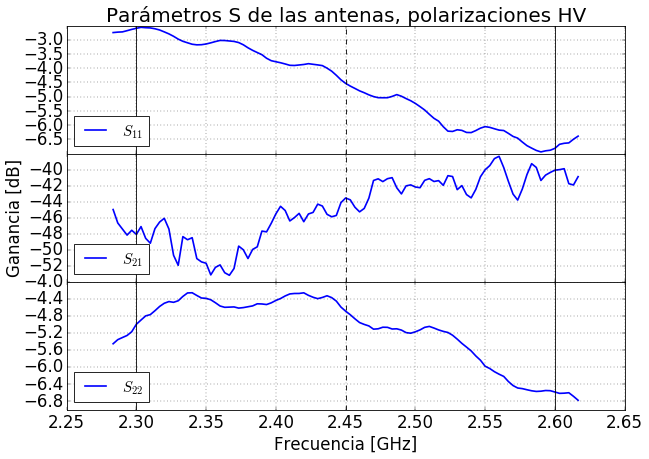
\includegraphics[width=7cm]{SParamsHV}
    \caption{Polarización HV}
    \label{subfig:hvPol}
  \end{subfigure}

  \begin{subfigure}{0.47\textwidth}
    \centering
    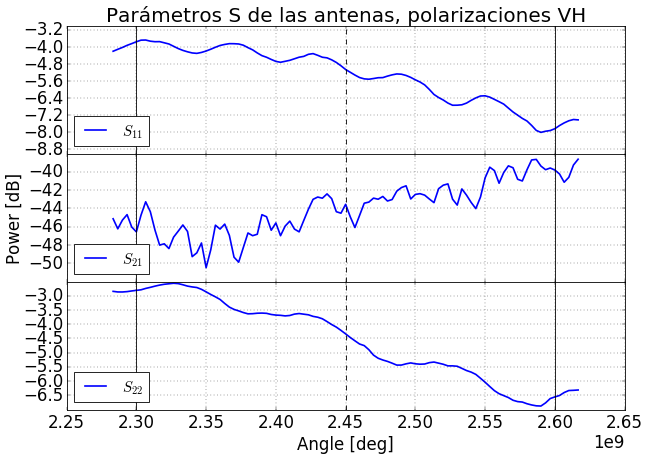
\includegraphics[width=7cm]{SParamsVH}
    \caption{Polarización VH}
    \label{subfig:vhPol}
  \end{subfigure}
  \begin{subfigure}{0.47\textwidth}
    \centering
    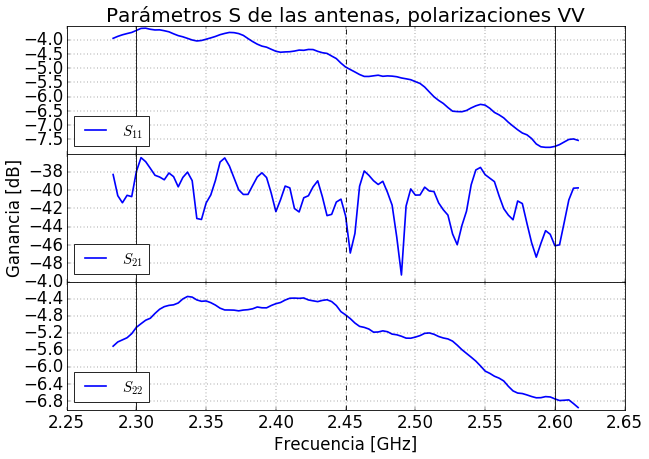
\includegraphics[width=7cm]{SParamsVV}
    \caption{Polarización VV}
    \label{subfig:vvPol}
  \end{subfigure}
  \caption{Mediciones de parámetros S de las antenas en todas las combinaciones de polarizaciones. \ref{subfig:hhPol} HH, \ref{subfig:hvPol} HV, \ref{subfig:vhPol} VH y \ref{subfig:vvPol} VV.}
  \label{fig:sParametersMeasurements}
\end{figure}

Se puede apreciar que si bien los coeficientes de reflexión son similares entre polarizaciones, todos muestran una gran variación de respuesta a lo largo de la frecuencia de trabajo, llegando a ser de hasta $\SI{4.6}{\dB}$. Por el lado de la variación del coeficiente de transmisión, la polarización HH solamente está en el orden de los $\SI{4.5}{\dB}$. En cambio para el resto de las polarizaciones, la misma resulta ser del orden de los $\SI{12}{\dB}$.

La tabla \ref{tab:antennasParameters} resume los valores medidos de cada parámetros S a la frecuencia central. Se puede apreciar que los coeficientes de reflexión de cada antena en cada polarización permanece invariante ante las combinaciones de polarizaciones utilizadas. A su vez, se puede apreciar que el coeficiente de transmisión directo permanece casi igual al coeficiente de transmisión inverso y que dichos coeficientes también son iguales entre las polarizaciones HV y VH. Por último, cabe destacar que las polarizaciones HH poseen un mayor coeficiente de transmisión que las VV en un orden de $\SI{8}{\dB}$.

\begin{table}[htb]
  \caption{Parámetros S de las antenas medidos con un VNA a frecuencia central.}
  \centering
  \label{tab:antennasParameters}
  \begin{tabular}{l *{4}{S[table-auto-round, table-format=-2.2]}}
  \toprule
  \multirow{2}{*}{\textbf{Parámetro S}} & \multicolumn{4}{c}{\textbf{Polarizaciones}} \tabularnewline
  \cmidrule{2-5}
  & HH & HV & VH & VV \tabularnewline
  \midrule
  
  $S_{11}$ & -4.46033873376335 & -4.53492363950625 & -5.06302223793916 & -4.95964466600015 \tabularnewline

  $S_{12}$ & -34.8204780020621 & -43.4389116307712 & -43.5577358595805 & -42.7387139376128 \tabularnewline

  $S_{21}$ & -34.7141043352772 & -43.5629806134325 & -43.4259094492972 & -42.8482094658858 \tabularnewline

  $S_{22}$ & -4.32197124367156 & -4.69545953806287 & -4.34205880309025 & -4.78356133012197 \tabularnewline

  \bottomrule
  \end{tabular}
\end{table}


\subsection{Diagrama de Radiación}

Para esta medición se desconectó del radar la antena receptora y se la conectó en el analizador de espectros a una distancia igual a $\SI{1.427}{\meter}$ para medir la potencia recibida por el radar, ver figura \ref{fig:radiationPatternConnections}. A la antena transmisora se la fue rotando a medida que se tomaban muestras para obtener el diagrama de radiación. Por último, tanto a la antena transmisora como la receptora se le fueron cambiando las polarizaciones para obtener el diagrama en todas las posibles combinaciones, HH, HV, VH y VV.
\begin{figure}[htb]
 \centering
 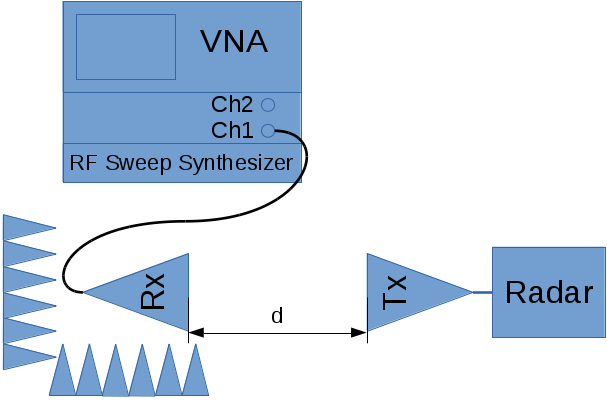
\includegraphics[width=8cm]{RadiatingPatternAntenaWorkbench}
 \caption{Banco de medición, diagrama de radiación entre antenas.}
 \label{fig:radiationPatternConnections}
\end{figure}

Es importante notar en la imagen \ref{fig:radiationPatternConnections} que la antena receptora se la colocó frente a absorbedores para disminuir la potencia recibida proveniente de ecos en las paredes de la sala en que se realizó la medición. La tabla \ref{tab:PNAConfigRadiationPattern} resume las configuraciones utilizadas en el analizador de espectros para las mediciones.

\begin{table}[H]
  \caption{Configuración del analizador de espectros, medición del diagrama de radiación.}
  \centering
  \label{tab:PNAConfigRadiationPattern}
  \begin{tabular}{l c c}
  \toprule
  \textbf{Característica} & \textbf{Configuración} & \textbf{Unidad} \tabularnewline
  \midrule
  Mode & ANALYZER & \tabularnewline

  Center Freq & 2434262820,514000 & \si{\hertz} \tabularnewline

  Freq Offset & 0,000000 & \si{\hertz} \tabularnewline

  Span & 100000000,000000 & \si{\hertz} \tabularnewline

  x-Axis & LIN & \tabularnewline

  Start & 2384262820,514000 & \si{\hertz} \tabularnewline

  Stop & 2484262820,514000 & \si{\hertz} \tabularnewline

  Ref Level & -9,000000 & \si{\dBm} \tabularnewline

  Level Offset & 0,000000 & \si{\dB} \tabularnewline

  Ref Position & 100,000000 & \si{\percent} \tabularnewline

  y-Axis & LOG & \tabularnewline

  Level Range & 100,000000 & \si{\dB} \tabularnewline

  Rf Att & 5,000000 & \si{\dB} \tabularnewline

  RBW & 2000000,000000 & \si{\hertz} \tabularnewline

  VBW & 50,000000 & \si{\hertz} \tabularnewline

  SWT & 2,500000 & \si{\second} \tabularnewline

  Trace Mode & CLR/WRITE & \tabularnewline

  Detector & RMS & \tabularnewline

  Sweep Count & 0 & \tabularnewline
  \bottomrule
  \end{tabular}
\end{table}

La tabla \ref{tab:antennaPattern} resume los resultados de las mediciones realizadas y la imagen \ref{fig:patterns} muestra los diagramas de radiación. Se puede observar que el ancho del lóbulo principal para las polarizaciones HH y VV son muy similares, aproximadamente de unos $\SI{50}{\degree}$ y que las ganancias máximas del mismo rondan los $\SI{-22}{\dB}$. En cambio, se nota que para HH los lóbulos secundarios son $\SI{3}{\dB}$ mayores y los mismos se encuentran a $\SI{3.8}{\dBc}$ para HH y $\SI{6.55}{\dBc}$ para VV.

Por último, comparando los gráficos co-polares con respecto al cross-polar, se puede observar que el rechazo por polarización cruzada es de $\SI{18}{\dB}$, dado que la ganancia recibida es de $\SI{-40}{\dB}$ frente a los $\SI{-22}{\dB}$ de las co-polares, para el centro del lóbulo principal. A su vez se observa que los lóbulos secundarios poseen una ganancia mayor, llegando a los $\SI{-37}{\dB}$.

\begin{figure}
  \centering
  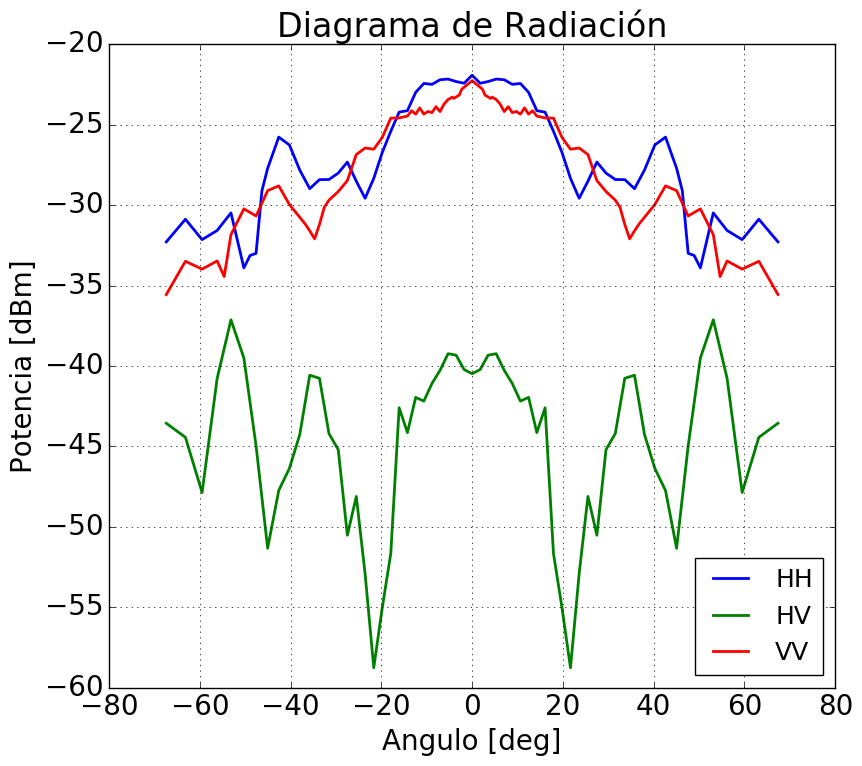
\includegraphics[width=10cm]{patterns}
  \caption{Diagrama de radiación del radar en distintas combinaciones de polarizaciones, HH, HV y VV.}
  \label{fig:patterns}
\end{figure}

\begin{table}[H]
  \caption{Mediciones diagrama de radiación entre polarizaciones.}
  \centering
  \label{tab:antennaPattern}
  \begin{tabular}{*{5}{S[table-auto-round, table-format=-2.2]}}
  \toprule
  \multirow{2}{*}{\textbf{ángulos entre antenas [$\si{\degree}$]}} & \multicolumn{4}{c}{\textbf{Potencia transmitida en polarizaciones}} \tabularnewline
  \cmidrule{2-5}
   & HH & HV & VH & VV \tabularnewline
  \midrule
  0.0 & -21.914052963256836 & -40.480464935302734 & -40.480464935302734 & -22.251615524291992 \tabularnewline

  1.91021317171 & -22.4134578704834 & -40.224273681640625 & -40.224273681640625 & -22.784189224243164 \tabularnewline

  3.82255372927 & -22.30802345275879 & -39.3284797668457 & -39.3284797668457 & -23.145263671875 \tabularnewline

  5.73917047727 & -22.154735565185547 & -39.235477447509766 & -39.235477447509766 & -23.423660278320312 \tabularnewline

  7.66225566077 & -22.194988250732422 & -40.26947021484375 & -40.26947021484375 & -24.174240112304688 \tabularnewline

  9.59406822686 & -22.48287582397461 & -41.09086608886719 & -41.09086608886719 & -24.239660263061523 \tabularnewline

  11.5369590328 & -22.42629051208496 & -42.18770980834961 & -42.18770980834961 & -24.336830139160156 \tabularnewline

  13.4933988216 & -22.981735229492188 & -41.95241928100586 & -41.95241928100586 & -24.332292556762695 \tabularnewline

  15.4660099534 & -24.11693000793457 & -44.143924713134766 & -44.143924713134766 & -24.45547866821289 \tabularnewline

  17.4576031237 & -24.21193504333496 & -42.601112365722656 & -42.601112365722656 & -24.572660446166992 \tabularnewline

  19.4712206345 & -25.39852523803711 & -51.66230010986328 & -51.66230010986328 & -24.58316993713379 \tabularnewline

  21.5101882669 & -26.707298278808594 & -55.01024627685547 & -55.01024627685547 & -25.775318145751953 \tabularnewline

  23.5781784782 & -28.32943344116211 & -58.773075103759766 & -58.773075103759766 & -26.516315460205078 \tabularnewline

  25.6792886195 & -29.568967819213867 & -52.928672790527344 & -52.928672790527344 & -26.44162368774414 \tabularnewline

  27.8181392847 & -28.507495880126953 & -48.11441421508789 & -48.11441421508789 & -26.84745216369629 \tabularnewline

  30.0 & -27.317434310913086 & -50.52842330932617 & -50.52842330932617 & -28.46544075012207 \tabularnewline

  32.2309526355 & -28.002696990966797 & -45.20555877685547 & -45.20555877685547 & -29.152206420898438 \tabularnewline

  34.5181078411 & -28.401615142822266 & -44.20515060424805 & -44.20515060424805 & -29.684959411621094 \tabularnewline

  36.8698976458 & -28.40848731994629 & -40.76640701293945 & -40.76640701293945 & -31.19536590576172 \tabularnewline

  39.2964802392 & -28.97147560119629 & -40.5757942199707 & -40.5757942199707 & -31.591350555419922 \tabularnewline

  41.8103148958 & -27.810001373291016 & -44.27327346801758 & -44.27327346801758 & -30.774405479 \tabularnewline

  44.4270040008 & -26.254615783691406 & -46.36780548095703 & -46.36780548095703 & -29.957460403442383 \tabularnewline

  47.1665719339 & -25.764413833618164 & -47.74458694458008 & -47.74458694458008 & -28.79700469970703 \tabularnewline

  50.0554948102 & -27.705350875854492 & -51.336891174316406 & -51.336891174316406 & -29.092802047729492 \tabularnewline

  53.1301023542 & -32.99269104003906 & -44.96973419189453 & -44.96973419189453 & -30.67097282409668 \tabularnewline

  56.4426902381 & -33.899192810058594 & -39.50574493408203 & -39.50574493408203 & -30.22670555114746 \tabularnewline

  60.0735651334 & -30.478853225708008 & -37.128719329833984 & -37.128719329833984 & -31.830547332763672 \tabularnewline

  64.1580672368 & -31.572757720947266 & -40.781593322753906 & -40.781593322753906 & -33.468048095703125 \tabularnewline

  68.9605302187 & -32.14019012451172 & -47.87135314941406 & -47.87135314941406 & -33.976505279541016 \tabularnewline

  75.164888418 & -30.873291015625 & -44.438751220703125 & -44.438751220703125 & -33.48764419555664 \tabularnewline

  90.0 & -32.28058624267578 & -43.56352233886719 & -43.56352233886719 & -35.55542755126953 \tabularnewline
  \bottomrule
  \end{tabular}
\end{table}


\section{Resumen}

En este capítulo se detallaron todos los subsistemas de hardware que componen al radar. Los mismos son el modulador, la cadena de RF, las antenas transmisoras y receptoras, el filtro pasa bajos y por último el gabinete. A su vez se midió cada uno de los mismos para verificar su correcto funcionamiento y cumplimiento de los requerimientos de nivel 2.

El circuito modulador fue construido de tal forma de poder transmitir más de un tipo de modulación ante la posibilidad de realizar futuros ensayos con distintos tipos de señales transmitidas, requerimiento \ref{req:l2_mod}. Las posibles modulaciones son diente de sierra creciente o decreciente, triangular y sinusoidal.

La potencia transmitida por la cadena de RF sin modular es igual a $\SI{1.87}{\dBm}$, al modular con el diente de sierra se obtiene un ancho de banda igual a $\SI{291.67}{\MHz}$.

Tanto para aumentar la directividad de las antenas como para que cada una sea polarimétrica, se hace uso de cavidades, que por simplicidad son cilíndricas. En un paso futuro, para asegurar la polarimetría se deben utilizar prismas rectangulares y para disminuir el cross-talk entre polarizaciones de una misma antena, se debe separar cada monopolo en una longitud de onda. Con respecto a las mediciones de comportamiento de las antenas, se puede observar que el coeficiente de reflexión ronda los $\SI{-5}{\dB}$ y que los coeficientes de transmisión entre polarizaciones ronda los $\SI{-43}{\dB}$ salvo para HH que ronda los $\SI{-35}{\dB}$.

Por último, se midió el diagrama de radiación a una distancia de $\SI{1.427}{\meter}$, se puede determinar que el rechazo de polarización cruzada es de $\SI{18}{\dB}$ siendo la ganancia recibida del centro del lóbulo principal para el caso co-polar igual a $\SI{-22}{\dB}$. Por último, los lóbulos secundarios se encuentran a $\SI{50}{\degree}$ y los mismos poseen una potencia de $\SI{3.8}{\dBc}$ para el caso HH y de $\SI{6.55}{\dBc}$ para el caso VV.

% \chapter{Resultados previstos} \label{ch:results}

A partir de las actividades propuestas en el plan se prevé:

\begin{enumerate}
    \item Obtener un simulador del funcionamiento del radar completo en donde se puedan modificar propiedades tanto de transmisión y recepción del radar como de distancia y propiedades del cuerpo iluminado.

    \item Armar el prototipo de ingeniería del radar FMCW.

    \item Validar y caracterizar los distintos subsistemas del radar construido.

    \item Identificar las principales fuentes de incertidumbres para la determinación experimental de la matriz de dispersión de un blanco con el radar construido.

    \item Establecer criterios de mejoras para disminuir y mantener controladas dichas fuentes de incertidumbres.
\end{enumerate}

% \chapter{Mediciones de Aplicación} \label{ch:measurements}

% **************************** Define Graphics Path **************************
\ifpdf
    \graphicspath{{Chapter5/Figs/Raster/}{Chapter5/Figs/PDF/}{Chapter5/Figs/}}
\else
    \graphicspath{{Chapter5/Figs/Vector/}{Chapter5/Figs/}}
\fi

En este capítulo se realizan diferentes tipos de mediciones de aplicación. El mismo se encuentra dividido en dos secciones, la primera trata sobre ensayos aplicados en el simulador, para estudiar el efecto de la utilización de un objeto externo para la medición de la distancia entre el radar y el objeto a medir. La segunda sección resume los resultados obtenidos de las mediciones tomadas con el radar sobre un gabinete metálico y un corner reflector ante distintas distancias.


\section{Mediciones con Simulador}

En esta sección se realizan dos simulaciones para determinar la dependencia de la medición de los parámetros S del blanco iluminado con respecto a variaciones en la determinación de la distancia entre el objeto y el radar. 

En la figura \ref{fig:DistDependencySim} se observa que la distancia entre el mezclador y el blanco está determinada por la distancia real, $D$, sumada a un error, $\Delta D$. En la primer medición se tratará al error ($\Delta D$) como una variable conocida y configurable, en cambio, para la segunda medición se la tratará como una incertidumbre.

\begin{figure}[H]
  \centering
  \includegraphics[width=12cm]{distanceDependency}
  \caption{Medición de propiedades del blanco ante diferentes diferencias de distancias.}
  \label{fig:DistDependencySim}
\end{figure}

Para disminuir el tiempo de procesamiento, se configuró el ancho de banda y la frecuencia central de la señal transmitida. Los valores son $\SI{300}{\kHz}$ y $\SI{2450}{\kHz}$ respectivamente. Dado que dichos parámetros son 3 órdenes de magnitud menores que la del radar, la resolución en rango simulada es 3 órdenes de magnitud mayor. Por lo tanto, las distancias a simular se incrementarán de la misma manera.


\subsection{Dependencia con la distancia}

En esta sección se estudia la dependencia de la medición de un componente de la matriz de dispersión asociada al blanco iluminado con respecto a un error en la determinación de la distancia. Para ello, se simula que la distancia medida por el radar, $D_{medida}$, está determinada por la ecuación \ref{eq:distError}, siendo $D$ la distancia real entre el blanco y el radar y $\Delta D$ es un error conocido configurable.
\begin{equation} \label{eq:distError}
  D_{medida} = D - \Delta D
\end{equation}

\begin{table}[htb]
  \caption{Componente HH de la Matriz de dispersión del blanco a distintas distancias utilizando el simulador.}
  \centering
  \label{tab:simDeltaDist}
  \begin{tabular}{l *{4}{S[table-auto-round, table-format=1.1] S[table-auto-round, table-format=-3]}}
  \toprule
  \multirow{4}{1cm}{\textbf{Delta [m]}} & \multicolumn{8}{c}{\textbf{Distancia [m]}} \tabularnewline
  \cmidrule{2-9}
   & \multicolumn{2}{c}{30,760} & \multicolumn{2}{c}{35000} & \multicolumn{2}{c}{37760,1695} & \multicolumn{2}{c}{40000} \tabularnewline
  \cmidrule(r){2-3} \cmidrule(lr){4-5} \cmidrule(lr){6-7} \cmidrule(l){8-9}
   & {Gain} & {Phase} & {Gain} & {Phase} & {Gain} & {Phase} & {Gain} & {Phase} \tabularnewline
   & [$\si{\deci\bel}$] & [$\si{\degree}$] & [$\si{\deci\bel}$] & [$\si{\degree}$] & [$\si{\deci\bel}$] & [$\si{\degree}$] & [$\si{\deci\bel}$] & [$\si{\degree}$] \tabularnewline
  \midrule
  
  0 & 0.9974998783 & -0.8999873159 & 0.9970854521 & 5.0829022535 & 0.9974244573 & 0.0563536612 & 0.9991246271 & 1.1021289469 \tabularnewline

  5 & 0.996851467 & -28.5141663823 & 0.9965158111 & -22.5305974732 & 0.9968962677 & -27.5567038267 & 0.9986251585 & -26.5105696718 \tabularnewline

  10 & 0.9962033718 & -56.1283462497 & 0.9959464141 & -50.1440980009 & 0.9963682879 & -55.1697621157 & 0.9981258771 & -54.1232690916 \tabularnewline

  40 & 0.9923214343 & 138.1865577226 & 0.9925351551 & 144.1748820091 & 0.9932048122 & 139.1518713272 & 0.9951341194 & 140.2005175668 \tabularnewline

  100 & 0.984591606 & 166.8162791476 & 0.9857389337 & 172.8127555094 & 0.986900466 & 167.7950516932 & 0.9891707856 & 168.8480043635 \tabularnewline

  \bottomrule 
  \end{tabular}
\end{table}

La tabla \ref{tab:simDeltaDist} resume el componente HH de la matriz de dispersión obtenidos ante errores en la determinación de la distancia. La columna Delta indica el valor adoptado en la variable $\Delta D$ de la ecuación \ref{eq:distError}. Se puede observar que la variación que tiene $\Delta D$ en la determinación de la distancia en el resultado es despreciable para la ganancia, en cambio, para la fase, es totalmente determinante. Un acercamiento del blanco al radar de $\SI{5}{\meter}$ implica que la señal recorre $\SI{10}{\meter}$ menos, dado que la misma recorre el mismo camino dos veces. A su vez, independientemente de la distancia a la que está el blanco, un error igual a $\SI{5}{\meter}$ implica un desfase igual a $\SI{-28}{\degree}$. Este resultado es el esperado dado que la longitud de onda de la señal transmitida es aproximadamente $\SI{122}{\meter}$, por lo tanto un error de $\SI{12.2}{\meter}$ implica un desfase de $\SI{36}{\degree}$.

La figura \ref{fig:deltaDistSim} muestra de forma separada las mediciones de la ganancia y fase del blanco en las distancias $\SI{30760}{\meter}$, $\SI{35000}{\meter}$, $\SI{37760.1695}{\meter}$ y $\SI{40000}{\meter}$. Los valores del gráfico de fase no coinciden con la tabla dado que, para enfatizar la linealidad de dicha variable con respecto a la distancia, se restaron $\SI{360}{\degree}$ cuando era necesario.
\begin{figure}[H]
  \centering
  \begin{subfigure}{0.49\textwidth}
    \includegraphics[width=7cm]{deltaDistGain}
    \caption{Ganancia}
  \end{subfigure}
  \begin{subfigure}{0.49\textwidth}
    \includegraphics[width=7cm]{deltaDistPhase}
    \caption{Fase}
  \end{subfigure}
  \caption{Dependencia de la matriz de dispersión del blanco ante errores en la medición de la distancia al blanco.}
  \label{fig:deltaDistSim}
\end{figure}


\subsection{Incertidumbre en distancia}

En esta sección se introducen incertidumbres en la medición de la distancia buscando determinar cómo afecta a la medición de la matriz de dispersión del blanco iluminado. Dichas incertidumbres se las toma como ruido AWGN, por lo tanto poseen una distribución gaussiana con desvío estándar configurable y media igual a cero. La tabla \ref{tab:simIncertDist} resume los resultados obtenidos de la simulación de montecarlo con 1000 realizaciones.

\begin{table}[htb]
  \caption{Incertidumbre absoluta en el componente HH de la matriz de dispersión del blanco ante incertidumbre en la medición de distancia.}
  \centering
  \label{tab:simIncertDist}
  \begin{tabular}{l *{4}{S[table-auto-round, table-format=-1.3] S[table-auto-round, table-format=-3]}}
  \toprule
  \multirow{4}{1cm}{\textbf{Std [m]}} & \multicolumn{8}{c}{\textbf{Distancia [m]}} \tabularnewline
  \cmidrule{2-9}
   & \multicolumn{2}{c}{30760} & \multicolumn{2}{c}{35000} & \multicolumn{2}{c}{37760,1695} & \multicolumn{2}{c}{40000} \tabularnewline
  \cmidrule(r){2-3} \cmidrule(lr){4-5} \cmidrule(lr){6-7} \cmidrule(l){8-9}
   & {$\Delta Gain$} & {$\Delta Phase$} & {$\Delta Gain$} & {$\Delta Phase$} & {$\Delta Gain$} & {$\Delta Phase$} & {$\Delta Gain$} & {$\Delta Phase$} \tabularnewline
   & [$\si{\deci\bel}$] & [$\si{\degree}$] & [$\si{\deci\bel}$] & [$\si{\degree}$] & [$\si{\deci\bel}$] & [$\si{\degree}$] & [$\si{\deci\bel}$] & [$\si{\degree}$] \tabularnewline
  \midrule
  
  0 & 0.00 & 0.00 & 0.00 & 0.00 & 0.00 & 0.00 & 0.00 & 0.00 \tabularnewline

  5 & 0.000369507 & 15.7325843211 & 0.0003330912 & 16.1431290009 & 0.0002977873 & 15.5648756904 & 0.0002884168 & 15.9418570692 \tabularnewline

  10 & 0.0007337078 & 31.239336556 & 0.0006511433 & 31.5574962315 & 0.0006150956 & 32.1497974883 & 0.0005796089 & 32.0371315787 \tabularnewline

  40 & 0.0029849535 & 116.5644598149 & 0.002650077 & 116.673494049 & 0.0023426065 & 112.3447856255  & 0.0023238051 & 117.0437670382 \tabularnewline

  \bottomrule 
  \end{tabular}
\end{table}

Se puede observar que la variación en el resultado para la determinación de la ganancia es despreciable, en cambio, para la fase es totalmente determinante. Cabe destacar que la incertidumbre obtenida no depende de la distancia a la que se encuentra el blanco con respecto al radar.

La figura \ref{fig:incertDistSim} muestra la dependencia lineal entre la incertidumbre de la medición de la fase del blanco y el desvío estándar de la distancia al cual se encuentra. Se puede observar que, para cumplir con el requerimiento \ref{req:l1_phase}, y no tener una incertidumbre absoluta mayor a $\SI{30}{\degree}$, no se debe tener una incertidumbre en la distancia mayor a $\SI{8.33}{\meter}$.
\begin{figure}[H]
  \centering
  \includegraphics[width=7cm]{incertDistPhase}
  \caption{Medición de fase del blanco ante diferentes incertidumbres en distancias.}
  \label{fig:incertDistSim}
\end{figure}

\section{Mediciones con Radar}

En esta sección se realizan cuatro tipos de mediciones de aplicación con el radar utilizando diferentes blancos. En el primer caso se utiliza un gabinete rectangular frente a paneles absorbedores para disminuir los ecos en las paredes de la sala. En el segundo caso se estudia la dependencia de la estimación de la matriz de dispersión al tomar una distancia diferente a la real. Luego, en el tercer caso, se estudia el efecto de la presencia de incertidumbre en la distancia. Por último, en el cuarto caso, se mide un corner reflector.


\subsection{Medición de un gabinete metálico}

En esta sección se realizan diferentes mediciones variando la distancia entre el gabinete y el radar. Para disminuir el eco recibido de las paredes que se encuentran detrás del gabinete, se colocan paneles absorbedores. El objetivo de esta medición es la de determinar fuentes de incertidumbres que no se hayan tenido en cuenta previamente. Las imágenes de la figura \ref{fig:DistDependencySim2} muestran el ambiente de trabajo.
\begin{figure}[H]
  \centering
  \begin{subfigure}{0.59\textwidth}
    \includegraphics[width=9cm]{distanceDependencyRadar}
  \end{subfigure}
  \begin{subfigure}{0.39\textwidth}
    \includegraphics[width=6cm]{caseMeasurement}
  \end{subfigure}
  \caption{Medición de propiedades de un gabinete metálico ante diferentes distancias.}
  \label{fig:DistDependencySim2}
\end{figure}

La tabla \ref{tab:radarMeasurementResults} resume los resultados obtenidos. El error absoluto en las mediciones equivale a tres veces el desvío estándar, dado que se toma como hipótesis la de estar trabajando con una incertidumbre con distribución gaussiana.

\begin{table}[H]
  \caption{Matriz de dispersión del gabinete metálico medidos con el radar.}
  \centering
  \label{tab:radarMeasurementResults}
  \begin{tabular}{c c | *{2}{S[table-auto-round, table-format=1.3]} *{2}{S[table-auto-round, table-format=-2.2]} S[table-auto-round, table-format=-3] S[table-auto-round, table-format=2]}
  \toprule
  \textbf{Rango} & \textbf{Pol} & \textbf{Rango} & \textbf{$\Delta$Rango}  & \textbf{Gain} & \textbf{$\Delta$Gain} & \textbf{Phase} & \textbf{$\Delta$Phase} \tabularnewline

  [$\si{\meter}$] & & [$\si{\meter}$] & [$\si{\meter}$] & [$\si{\dB}$] & [$\si{\dB}$] & [$\si{\degree}$] & [$\si{\degree}$] \tabularnewline
  \midrule
  
  \multirow{4}{*}{1,32} & HH & 2.201 & 0.013 & 31.4539 & 0.0915 & 4.5 & 69.8 \tabularnewline
   & HV & 2.204 & 0.015 & 22.9796 & 0.1261 & -131.1 & 81.0 \tabularnewline
   & VH & 2.425 & 0.023 & 25.3829 & 0.2481 & -140.8 & 80.4 \tabularnewline
   & VV & 1.399 & 0.007 & 17.0184 & 0.1307 & 97.1 & 37.2 \tabularnewline

  \cmidrule{2-8}
  \multirow{4}{*}{1,56} & HH & 1.572 & 0.005 & 24.4271 & 0.0654 & -118.9 & 30.0 \tabularnewline
   & HV & 1.738 & 0.008 & 18.8475 & 0.0839 & -78.8 & 42.0 \tabularnewline
   & VH & 1.338 & 0.007 & 12.3065 & 0.0954 & 30.5 & 39.7 \tabularnewline
   & VV & 1.630 & 0.006 & 22.9165 & 0.1030 & -102.1 & 37.1 \tabularnewline

  \cmidrule{2-8}
  \multirow{4}{*}{1,71} & HH & 1.709 & 0.006 & 26.4757 & 0.0651 & 174.5 & 31.9 \tabularnewline
   & HV & 2.929 & 0.004 & 23.9049 & 0.0759 & -65.9 & 19.6 \tabularnewline
   & VH & 2.343 & 0.007 & 22.0027 & 0.0613 & -99.0 & 36.5 \tabularnewline
   & VV & 1.685 & 0.008 & 22.982 & 0.1295 & 58.9 & 49.5 \tabularnewline

  \cmidrule{2-8}
  \multirow{4}{*}{1,84} & HH & 1.994 & 0.006 & 28.0666 & 0.0532 & -90.1 & 33.6 \tabularnewline
   & HV & 1.224 & 0.007 & 5.9869 & 0.1663 & -61.1 & 40.2 \tabularnewline
   & VH & 2.258 & 0.006 & 18.3366 & 0.0649 & -1.3 & 31.9 \tabularnewline
   & VV & 2.072 & 0.003 & 26.4441 & 0.0632 & -73.7 & 22.2 \tabularnewline

  \cmidrule{2-8}
  \multirow{4}{*}{2,005} & HH & 2.364 & 0.008 & 30.0745 & 0.0695 & -190.8 & 43.1 \tabularnewline
   & HV & 3.896 & 0.013 & 25.8801 & 0.1221 & 10.7 & 71.8 \tabularnewline
   & VH & 2.259 & 0.006 & 18.1211 & 0.0513 & -7.8 & 35.5 \tabularnewline
   & VV & 2.108 & 0.005 & 24.5758 & 0.0572 & 15.0 & 28.8 \tabularnewline

  \bottomrule
  \end{tabular}
\end{table}

Analizando los resultados obtenidos en la tabla \ref{tab:radarMeasurementResults}, se pueden obtener las siguientes conclusiones:
\begin{description}
  \item[Determinación de la distancia] Se puede observar que se determina erróneamente la distancia al blanco. Esto se debe a que no se realizó una medición previa del clutter de la sala para substraer dicho efecto. En la figura \ref{fig:distanceError} se observa la FFT de la señal recibida, en la cual se indica que la potencia de la señal que se corresponde al eco del blanco es menor que la del propio clutter. De esta forma, se determina de una forma errónea la distancia al blanco.

  A su vez, se observa que sistemáticamente la ganancia para la polarización HH es mayor que para el resto. Dicho comportamiento se debe a que el crosstalk entre las antenas para dicha combinación de polarizaciones es la máxima medida, ver la sección \ref{ssc:sParameters}.

  \begin{figure}[H]
    \centering
    \includegraphics[width=15cm]{distanceError}
    \caption{FFT del eco recibido por el radar. Se observa que la potencia del eco recibido por el blanco es menor que el del clutter.}
    \label{fig:distanceError}
  \end{figure}

  \item[Determinación de Ganancia] Se puede observar que se determina erróneamente la relación de ganancia entre la señal incidente y reflejada del blanco. Esto se debe a tres causas principales. La primera se debe a que, como se mide de forma incorrecta la distancia al blanco, la atenuación real que impone el medio sobre la señal no es la calculada. La segunda está relacionada a que no se tomó en cuenta que el control del volumen de la computadora estaba en modo automático, por lo tanto entre ensayo y ensayo se modificó el nivel de la señal recibida, introduciendo un error grosero en dicha magnitud. La tercera se debe a que, como se puede observar en la figura \ref{fig:distanceError}, los niveles de potencia de la señal recibida son principalmente del clutter del ambiente. La mejor solución de este problema es la de realizar una medición previa del clutter sin blanco para realizar la resta de señales.

  \item[Determinación de Fase] Se puede observar que se determina erróneamente la relación de fase entre la señal incidente y reflejada del blanco. Esto es debe a dos causas principales. La primera se debe a que, como se mide de forma incorrecta la distancia al blanco, el desfase real que impone el medio sobre la señal no es la calculada. La segunda se debe a que, como no se eliminó el clutter de la señal, la medición resulta afectada.
\end{description}


\subsection{Dependencia con la distancia}

En esta sección se estudia la dependencia de la medición de los parámetros S del blanco iluminado con respecto a un error en la determinación de la distancia. Para ello, se introduce en el procesador de la señal recibida del radar la distancia al blanco según la ecuación \ref{eq:distErrorRadar}. En donde $D$ es la distancia real entre el blanco y el radar y $\Delta D$ es un valor configurable. 
\begin{equation} \label{eq:distErrorRadar}
  D_{medida} = D - \Delta D
\end{equation}

\begin{table}[H]
  \caption{Componente HH de la matriz de dispersión del blanco a distintas distancias utilizando el radar.}
  \centering
  \label{tab:simDeltaDistRadar}
  \begin{tabular}{l *{3}{S[table-auto-round, table-format=-1.2] S[table-auto-round, table-format=-3]}}
  \toprule
  \multirow{4}{1cm}{\textbf{Delta [$\si{\milli\meter}$]}} & \multicolumn{6}{c}{\textbf{Distancia [$\si{\meter}$]}} \tabularnewline
  \cmidrule{2-7}
   & \multicolumn{2}{c}{2,201} & \multicolumn{2}{c}{2,229} & \multicolumn{2}{c}{2,255} \tabularnewline
  \cmidrule(r){2-3} \cmidrule(lr){4-5} \cmidrule(l){6-7}
   & {Gain} & {Phase} & {Gain} & {Phase} & {Gain} & {Phase} \tabularnewline
   & [$\si{\dB}$] & [$\si{\degree}$] & [$\si{\dB}$] & [$\si{\degree}$] & [$\si{\dB}$] & [$\si{\degree}$] \tabularnewline
  \midrule
  
  0 & -1.8092 & 147.7 & -1.8941 & 133.2 & -1.4372 & 152.1 \tabularnewline

  5 & -1.8570 & 174.8 & -1.9362 & 161.4 & -1.4903 & 179.8 \tabularnewline

  10 & -1.8940 & 202 & -1.9772 & 188.0 & -1.5177 & 207.0 \tabularnewline

  15 & -1.9243 & 229.5 & -2.0172 & 215.5 & -1.5622 & 234.4 \tabularnewline

  \bottomrule 
  \end{tabular}
\end{table}
La tabla \ref{tab:simDeltaDistRadar} resume los componentes HH de la matriz de dispersión obtenidos ante errores en la determinación de la distancia. La columna Delta indica el valor adoptado en la variable $\Delta D$ de la ecuación \ref{eq:distErrorRadar}. Se puede observar que la variación en el resultado para la determinación de la ganancia resulta despreciable dado que al haber $\SI{15}{\milli\meter}$ de diferencia la medición disminuyó en $\SI{0.12}{\dB}$ y para el caso de la fase es totalmente determinante. Cabe destacar que un error en la medición de distancia de $\SI{5}{\milli\meter}$ implica que la señal recorre $\SI{10}{\milli\meter}$ menos, dado que la misma recorre el mismo camino dos veces. A su vez, independientemente de la distancia a la que está el blanco, un error igual a $\SI{5}{\milli\meter}$ implica un desfase igual a $\SI{27.6}{\degree}$. Este resultado es el esperado dado que la longitud de onda de la señal transmitida es aproximadamente $\SI{122}{\milli\meter}$, por lo tanto un error de $\SI{12.2}{\meter}$ implica un desfase de $\SI{36}{\degree}$.

\begin{figure}[H]
  \centering
  \begin{subfigure}{0.49\textwidth}
    \includegraphics[width=7cm]{deltaDistGainRadar}
    \caption{Ganancia}
  \end{subfigure}
  \begin{subfigure}{0.49\textwidth}
    \includegraphics[width=7cm]{deltaDistPhaseRadar}
    \caption{Fase}
  \end{subfigure}
  \caption{Parámetros S del blanco a distintas distancias.}
  \label{fig:deltaDistRadar}
\end{figure}
La figura \ref{fig:deltaDistRadar} muestra de forma separada las mediciones de la ganancia y fase del blanco en las distancias $\SI{2.201}{\meter}$, $\SI{2.229}{\meter}$ y $\SI{2.255}{\meter}$. Se puede observar que tanto la ganancia como el desfase son del mismo orden para cada distancia.


\subsection{Incertidumbre en Distancia} \label{ssc:distIncert}

En esta sección se estudia la dependencia de las incertidumbres obtenidas de los parámetros S del blanco iluminado con respecto a la incertidumbre de la distancia. Para ello se analiza la misma adquisición dos veces, la primera introduciendo la distancia en el programa, y en la segunda utilizando el rango determinado por el radar.

La tabla \ref{tab:radarDistIncert} está dividida en dos partes. A la izquierda de la misma se muestran las incertidumbres obtenidas sin incertidumbre en distancia. En cambio, a la derecha, se muestran dichos resultados con incertidumbre en distancia.

\begin{table}[H]
  \caption{Dependencia de incertidumbre de los parámetros S medidos ante incertidumbre en la distancia.}
  \centering
  \label{tab:radarDistIncert}
  \begin{tabular}{c c | S[table-auto-round, table-format=1.1] S[table-auto-round, table-format=2] || *{2}{S[table-auto-round, table-format=-2.2]} S[table-auto-round, table-format=1.1] S[table-auto-round, table-format=3]}
  \toprule
  \textbf{Rango} & \textbf{Pol} & \textbf{$\Delta$Gain} & \textbf{$\Delta$Phase} & \textbf{Rango} & \textbf{$\Delta$Rango}  & \textbf{$\Delta$Gain} & \textbf{$\Delta$Phase} \tabularnewline

  [$\si{\meter}$] & & [$\si{\dB}$] & [$\si{\degree}$] & [$\si{\meter}$] & [$\si{\meter}$] & [$\si{\dB}$] & [$\si{\degree}$] \tabularnewline
  \midrule

  \multirow{4}{*}{2,201} & HH & 0.4531 & 9.1 & 2.201 & 0.011 & 0.4921 & 56.3 \tabularnewline
   & HV & 1.5631 & 13.9 & 2.247 & 0.026 & 1.5951 & 163.6 \tabularnewline
   & VH & 2.1342 & 87.1 & 2.288 & 0.036 & 2.205 & 204.8 \tabularnewline
   & VV & 0.3614 & 7.3 & 2.195 & 0.014 & 0.3789 & 82.1 \tabularnewline

  \bottomrule
  \end{tabular}
\end{table}

Analizando los resultados de la tabla \ref{tab:radarDistIncert}, se puede llegar a la conclusión que la incertidumbre en la ganancia no se ve afectada ante la eliminación de la incertidumbre en la distancia. En cambio, se puede observar una fuerte dependencia de la incertidumbre de fase con respecto a la incertidumbre de distancia.


\subsection{Medición de un Corner Reflector}

Para esta experiencia se construye un corner reflector triangular de $\SI{50}{\centi\meter}$ de lado, ver figura \ref{fig:corner}. El máximo RCS que se puede obtener, siguiendo la ecuación \ref{eq:theoreticalRcs}, es igual a $\SI{12.43}{\dB}$.
\begin{figure}[H]
  \centering
  \includegraphics[width=6cm]{cornerReflector}
  \caption{Corner reflector construido de $\SI{50}{\centi\meter}$ de lado para realizar las mediciones.}
  \label{fig:corner}
\end{figure}

La disposición del radar y del corner reflector en la sala se muestra en las imágenes de la  figura \ref{fig:cornerMeasurement}. Se puede determinar que el ángulo de incidencia con respecto a la horizontal resulta del orden de $\SI{24}{\degree}$. Por lo tanto, se espera una disminución de $\SI{3}{\dB}$, la cual se determina en la figura \ref{fig:cornerRel}. A su vez, en la figura \ref{fig:cornerErrors} se muestra cómo el RCS resulta afectado ante la pérdida de ortogonalidad entre las caras del corner. Se espera que haya una pérdida extra del orden de los $\SI{10}{\dB}$.
\begin{figure}
  \centering
  \begin{subfigure}{0.54\textwidth}
    \includegraphics[width=8cm]{cornerMeasurementScheme}
  \end{subfigure}
  \begin{subfigure}{0.44\textwidth}
    \includegraphics[width=6.5cm]{cornerMeasurement}
  \end{subfigure}
  \caption{Medición de propiedades del corner reflector ante diferentes distancias.}
  \label{fig:cornerMeasurement}
\end{figure}
La tabla \ref{tab:cornerMeasurementResults} resume los resultados obtenidos. El error absoluto en las mediciones equivale a tres veces el desvío estándar, dado que se toma como hipótesis la de estar trabajando con una incertidumbre con distribución gaussiana. Dado que se obtienen mejores resultados de fase midiendo la distancia del radar al blanco de forma externa, ver la sección \ref{ssc:distIncert} Incertidumbre en Distancia, se utiliza una cinta métrica para dichas mediciones. Por último, las mediciones se realizaron en dos etapas, primero se mide el clutter, adquisición sin el blanco y luego con el blanco, restando el clutter medido previamente.

\begin{table}[H]
  \caption{Parámetros de dispersión del corner reflector medidos con el radar.}
  \centering
  \label{tab:cornerMeasurementResults}
  \begin{tabular}{c c | S[table-auto-round, table-format=1.2] S[table-auto-round, table-format=1.2] S[table-auto-round, table-format=-2.2] S[table-auto-round, table-format=1.2] S[table-auto-round, table-format=-3] S[table-auto-round, table-format=2]}
  \toprule
  \textbf{Rango} & \textbf{Pol} & \textbf{Rango} & \textbf{$\Delta$Rango}  & \textbf{Gain} & \textbf{$\Delta$Gain} & \textbf{Phase} & \textbf{$\Delta$Phase} \tabularnewline

  [$\si{\meter}$] & & [$\si{\meter}$] & [$\si{\meter}$] & [$\si{\dB}$] & [$\si{\dB}$] & [$\si{\degree}$] & [$\si{\degree}$] \tabularnewline
  \midrule

  \multirow{4}{*}{2,201} & HH & 2.201 & 0.011 & -1.3969 & 0.4531 & -7.8 & 9.1 \tabularnewline
   & HV & 2.247 & 0.026 & -14.0225 & 1.5631 & -73.1 & 13.9 \tabularnewline
   & VH & 2.288 & 0.036 & -14.1252 & 2.1342 & -92.4 & 87.1 \tabularnewline
   & VV & 2.195 & 0.014 & -1.8092 & 0.3614 & 147.7 & 7.3 \tabularnewline

  \cmidrule{2-8}
  \multirow{4}{*}{2,229} & HH & 2.223 & 0.017 & -1.2961 & 0.3128 & -11.0 & 9.3 \tabularnewline
   & HV & 2.313 & 0.041 & -13.3133 & 1.5806 & -71.5 & 14.0 \tabularnewline
   & VH & 2.317 & 0.038 & -14.7132 & 2.3655 & -93.3 & 87.3 \tabularnewline
   & VV & 2.246 & 0.023 & -1.8941 & 0.2935 & 133.2 & 12.3 \tabularnewline

  \cmidrule{2-8}
  \multirow{4}{*}{2,255} & HH & 2.26 & 0.01 & -1.6825 & 0.4407 & -4.0 & 5.2 \tabularnewline
   & HV & 2.305 & 0.038 & -14.2542 & 1.2031 & -59.7 & 18.3 \tabularnewline
   & VH & 2.359 & 0.049 & -13.4975 & 1.8296 & -95.4 & 33.8 \tabularnewline
   & VV & 2.245 & 0.019 & -1.4372 & 0.3531 & 152.1 & 7.8 \tabularnewline

  \cmidrule{2-8}
  \multirow{4}{*}{2,285} & HH & 2.272 & 0.021 & -1.9684 & 0.4278 & -3.23 & 9.9 \tabularnewline
   & HV & 2.398 & 0.039 & -14.3538 & 1.1613 & -83.6 & 16.9 \tabularnewline
   & VH & 2.379 & 0.052 & -14.1736 & 1.5638 & -95.2 & 60.2 \tabularnewline
   & VV & 2.287 & 0.023 & -1.6621 & 0.3498 & 177.4 & 12.4 \tabularnewline

  \bottomrule
  \end{tabular}
\end{table}

Las figuras \ref{fig:measuredDistCorner}, \ref{fig:measuredGainCorner} y \ref{fig:measuredPhaseCorner} muestran las distancias, ganancias y desfases esperados y medidos por le radar asociados a sus respectivas incertidumbres con respecto a las distintas distancias medidas de forma externa. Se puede concluir lo siguiente:
\begin{figure}[H]
  \centering
  \begin{subfigure}{0.49\textwidth}
    \includegraphics[width=6cm]{measuredCornerRangeHH}
  \end{subfigure}
  \begin{subfigure}{0.49\textwidth}
    \includegraphics[width=6cm]{measuredCornerRangeHV}
  \end{subfigure}

  \begin{subfigure}{0.49\textwidth}
    \includegraphics[width=6cm]{measuredCornerRangeVH}
  \end{subfigure}
  \begin{subfigure}{0.49\textwidth}
    \includegraphics[width=6cm]{measuredCornerRangeVV}
  \end{subfigure}
  \caption{Distancia medida con su incertidumbre por el radar con respecto a la distancia medida con una cinta métrica.}
  \label{fig:measuredDistCorner}
\end{figure}
\begin{figure}[H]
  \centering
  \begin{subfigure}{0.49\textwidth}
    \includegraphics[width=6cm]{measuredCornerGainHH}
  \end{subfigure}
  \begin{subfigure}{0.49\textwidth}
    \includegraphics[width=6cm]{measuredCornerGainHV}
  \end{subfigure}

  \begin{subfigure}{0.49\textwidth}
    \includegraphics[width=6cm]{measuredCornerGainVH}
  \end{subfigure}
  \begin{subfigure}{0.49\textwidth}
    \includegraphics[width=6cm]{measuredCornerGainVV}
  \end{subfigure}
  \caption{Ganancia medida del blanco con su incertidumbre por el radar con respecto a la distancia medida con una cinta métrica.}
  \label{fig:measuredGainCorner}
\end{figure}
\begin{figure}[H]
  \centering
  \begin{subfigure}{0.49\textwidth}
    \includegraphics[width=6cm]{measuredCornerPhaseHH}
  \end{subfigure}
  \begin{subfigure}{0.49\textwidth}
    \includegraphics[width=6cm]{measuredCornerPhaseHV}
  \end{subfigure}

  \begin{subfigure}{0.49\textwidth}
    \includegraphics[width=6cm]{measuredCornerPhaseVH}
  \end{subfigure}
  \begin{subfigure}{0.49\textwidth}
    \includegraphics[width=6cm]{measuredCornerPhaseVV}
  \end{subfigure}
  \caption{Fase medida del blanco con su incertidumbre por el radar con respecto a la distancia medida con una cinta métrica.}
  \label{fig:measuredPhaseCorner}
\end{figure}


\begin{description}
  \item[Determinación de la distancia] En la figura \ref{fig:measuredDistCorner} se puede observar que el radar determina correctamente la distancia al blanco para las adquisiciones co-polares. En cambio, como el corner posee un alto rechazo para adquisiciones cross-polares, el radar detecta la presencia de otro cuerpo de la sala en que se realizaron las mediciones. Hay algunas adquisiciones co-polares en donde la distancia indicada por el radar es un par de centímetros mayor al ideal, esto se debe a que entre adquisiciones el blanco fue removido y vuelto a colocar sin volver a medir que el mismo quede exactamente en la misma posición. En la figura \ref{fig:correctDistance} se muestra la FFT de la señal recibida con el blanco luego de haber eliminado el clutter.

  \begin{figure}[H]
    \centering
    \includegraphics[width=15cm]{correctDistance}
    \caption{FFT del eco recibido por el radar. Se observa que la potencia del eco recibido por el blanco es mayor que el del clutter.}
    \label{fig:correctDistance}
  \end{figure}

  \item[Determinación de Ganancia] En la figura \ref{fig:measuredGainCorner} se puede observar que el radar mide correctamente las ganancias del corner reflector. Se aprecia una disminución de $\SI{14}{\dB}$ para adquisiciones cross-polares con respecto a las co-polares. A su vez, se puede apreciar que las adquisiciones co-polares poseen una ganancia del orden de los $\SI{-1.5}{\dB}$ con una incertidumbre absoluta de $\SI{1}{\dB}$.

  \item[Determinación de Fase] En la figura \ref{fig:measuredPhaseCorner} se puede observar que la relación de fase para la polarización HH es del orden de los $\SI{0}{\degree}$, en cambio para la VV resulta del orden de los $\SI{180}{\degree}$. En principio se espera que la respuesta sea la misma para ambas polarizaciones dado que, independientemente que el campo eléctrico sea paralelo o perpendicular al plano de incidencia al cuerpo, la relación entre el campo eléctrico reflejado e incidente a un plano metálico es aproximadamente igual a -1 \cite{Michelson1993}. Como el corner reflector posee tres caras, el desfase final esperable es igual a los $\SI{180}{\degree}$. Las adquisiciones con polarización HH poseen un desfase de $\SI{180}{\degree}$ con respecto a lo esperado debido a que la antena transmisora y receptora están espejadas entre sí. De esta forma, sumando $\SI{180}{\degree}$ a todas las mediciones de polarización HH se puede llegar a la conclusión que el radar detecta correctamente la relación de fase entre la señal incidente y reflejada del corner reflector para adquisiciones co-polares.

  A su vez, se puede observar que hay algunas mediciones para la polarización VV donde el valor está desfasado por unos $\SI{50}{\degree}$ del valor esperado. Esto se debe porque se utilizó la distancia medida con la cinta métrica en vez de la medida por el radar. Dado que de esta forma se obtiene una menor incertidumbre.

  Por último, la relación de fase para las adquisiciones cross-polares no se tienen que tomar en cuenta dado que el corner no responde a este tipo de adquisiciones.
\end{description}


\section{Resumen}

En este capítulo se realizaron mediciones de aplicación tanto con el simulador como con el radar.

Con el simulador se estudió la dependencia del resultado ante errores en la determinación de la distancia y ante incertidumbres en la misma. Para el primer caso la determinación de la ganancia es casi invariante, en cambio para la fase se puede observar que ante diferencias de distancia de $\lambda / 10$ se observan desfases de $\SI{36}{\degree}$. Para el segundo caso, se repiten los mismos resultados dado que si se desea tener una incertidumbre menor a $\SI{36}{\degree}$, se debe tener una incertidumbre menor a $\lambda / 10$ en la determinación de la distancia.

Con el radar se realizaron ensayos de la dependencia del resultado ante errores en la determinación de la distancia y ante incertidumbres en la misma. Se llegó a la conclusión que, para obtener mediciones de fase aceptables, es necesario utilizar instrumental externo, con menor incertidumbre asociada, para la medición de la distancia.

A su vez, se realizaron mediciones a distintas distancias con un gabinete rectangular y con un corner reflector. Con el primer caso se obtuvo que es necesario eliminar el clutter antes de obtener los parámetros del blanco iluminado. Esto se obtiene realizando la adquisición en dos pasos, primero sin el cuerpo y luego con el cuerpo. En el segundo caso se obtuvieron los resultados esperados, de esta forma se cumple con el requerimiento \ref{req:l0}.

% \chapter{Conclusiones} \label{ch:conclusions}

% **************************** Define Graphics Path **************************
\ifpdf
    \graphicspath{{Chapter6/Figs/Raster/}{Chapter6/Figs/PDF/}{Chapter6/Figs/}}
\else
    \graphicspath{{Chapter6/Figs/Vector/}{Chapter6/Figs/}}
\fi

\todo[inline]{* mejorar conclusiones, poniendo como mejorar ciertas cosas, amplificador del filtro pasa bajos, rango dinamico microfono de entrada a computadora}
\todo[inline]{* corregir ganancia en graficos de simulador/radar}
\todo[inline]{* poner grafico distancias corner reflector a radar}
\todo[inline]{* hacer seccion corner reflector a radar}
\todo[inline]{* poner grafico rango medido con su incertidumbre vs distancia real}
\todo[inline]{* poner ganancia medida vs distancias reales}
\todo[inline]{* poner fase medida sin compensar la distancia con sus incertidumbres}
\todo[inline]{* poner fase medida compensada con la distancia con sus incertidumbres}
\todo[inline]{* Agregar descripción de los botones referentes al volumen en capítulo 4.}
\todo[inline]{* Corregir algunos títulos de algunos gráficos....}
\todo[inline]{* Enviar video a rosa....}
\todo[inline]{* Corregir diagramas de clases en capítulo 4....}
\todo[inline]{* Add something to change from realTime application to file}

Como conclusiones de este trabajo se obtienen las siguientes conclusiones a saber

La obtención de los parámetros de dispersión no resulta sencillo dado que dicha tarea no solamente requiere tener cada parámetro de cada subsistema determinado y controlado para corregir su efecto en la señal, sino que también el entorno en que se realizan las mediciones afectan al resultado. Si no se posee una cámara anecoide o un ambiente abierto y despejado, el radar recibirá ecos de otros cuerpos o paredes de la sala de ensayos, modificando así los resultados de las mediciones.

Se observó que la incertidumbre en la medición de distancia entre el radar y el blanco iluminado tiene un efecto mucho mayor sobre la determinación del desfase que de la ganancia de los parámetros S del cuerpo. Si bien la potencia recibida posee una dependencia de orden cuatro con respecto a la distancia, una incertidumbre de $\SI{7}{\milli\meter}$ implica una incertidumbre absoluta total de ganancia igual a $\SI{0.06}{\dB}$. En cambio, como la longitud de onda de la señal es igual a $\SI{12.23}{\centi\meter}$, esto implica una incerteza asociada al desfase igual a $\SI{42}{\degree}$.

Dado que el diagrama de radiación de las antenas utilizadas es muy ancho, hay mucho crosstalk entre las antenas. Esto implica que los lóbulos secundarios de dicha señal afecta la medición de los parámetros S del blanco. Para mejorar este problema se puede cambiar el tipo de antena a un estilo patch, o utilizar reflectores con paredes corrugadas para suprimir ecos que vengan de los costados. Otro tipo de estrategia que se puede aplicar para disminuir aún más el crosstalk entre la antena transmisora y receptora, es la de aumentar la distancia entre las mismas.

Un aspecto importante a tener en cuenta a la hora de colocar las antenas es que no hayan componentes detras de las antenas, dado que las mismas emiten una gran cantidad de energía hacia dicha zona. La presencia de cualquier componente degradaría el diagrama de radiación final.

Por último, si bien se cumplieron con los objetivos plantese identificaron las modificaciones necesarias para mejorar el sistema en general con el objetivo de poder determinar los parámetros S del cuerpo con la menor incertidumbre posible.

% \chapter{Líneas Futuras} \label{ch:futureWork}

% **************************** Define Graphics Path **************************
\ifpdf
    \graphicspath{{Chapter6/Figs/Raster/}{Chapter6/Figs/PDF/}{Chapter6/Figs/}}
\else
    \graphicspath{{Chapter6/Figs/Vector/}{Chapter6/Figs/}}
\fi

A continuación se listan diversas modificaciones que se pueden aplicar tanto como para disminuir las incertidumbres asociadas como para realizar investigaciones de nuevas aplicaciones.

\mynote{para tirar abajo la hipótesis de que el comportamiento de los componentes no se modifica con la variación de temperatura se puede utilizar un esquema de calibración}

\mynote{no escribí nada sobre el corner reflector :D }
\begin{itemize}
    \item Para evitar la utilización de la misma señal para determinar tanto los parámetros S del blanco como la distancia entre el radar y el mismo, se puede disponer de un medidor de distancia láser externo.
    \item Se pueden aplicar distintas estrategias a la aplicada para suprimir el clutter para la medición.
    \item Se puede mejorar el procesador de señales para el caso que hayan más de un blanco iluminado a la vez.
    \item Se pueden cambiar las antenas para disminuir el crosstalk entre ellas y para obtener una mejor calidad de respuesta de sus parámetros S.
    \item Se puede incluir un sistema de calibración para calibrar la señal transmitida y recibida ante el cambio del comportamiento de los distintos subsistemas que componen el radar.
    \item Para realizar mediciones a mayores distancias se puede utilizar un ADC con una mayor frecuencia de muestreo y utilizar un filtro pasa bajos de mayor frecuencia de corte.
    \item Se puede aplicar un sistema para mejorar las alinealidades de la señal transmisora.
    \item Se puede realizar un estudio para determinar la mejor modulación de la señal a transmitir para la obtención del parámetros de dispersión del blanco iluminado.
    \item Se puede agregar un switch RF para poder elegir de forma automática las polarizaciones transmisoras y receptoras de forma automática.
    \item Se puede utilizar un conjunto de antenas para estudiar como se comporta este radar como un sistema SAR.
\end{itemize}



% ********************************** Back Matter *******************************
% Backmatter should be commented out, if you are using appendices after References
%\backmatter

% ********************************** Bibliography ******************************
\begin{spacing}{0.9}

% To use the conventional natbib style referencing
% Bibliography style previews: http://nodonn.tipido.net/bibstyle.php
% Reference styles: http://sites.stat.psu.edu/~surajit/present/bib.htm

% \bibliographystyle{apalike}
\bibliographystyle{unsrt} % Use for unsorted references
%\bibliographystyle{plainnat} % use this to have URLs listed in References
\cleardoublepage
\bibliography{References/Miniradar} % Path to your References.bib file


% If you would like to use BibLaTeX for your references, pass `custombib' as
% an option in the document class. The location of 'reference.bib' should be
% specified in the preamble.tex file in the custombib section.
% Comment out the lines related to natbib above and uncomment the following line.

%\printbibliography[heading=bibintoc, title={References}]


\end{spacing}

% ********************************** Appendices ********************************

% \begin{appendices} % Using appendices environment for more functunality

% \include{Appendix1/appendix1}
% \include{Appendix2/appendix2}

% \end{appendices}

% *************************************** Index ********************************
\printthesisindex % If index is present

\end{document}
